%!TEX root = ../appendix-C.tex
% ******************************* Thesis Appendix C: Figures ****************************

\chapter{Figures}
\label{chp:figures}

	\section{Diversity, Strength and Centrality in city networks}
	\label{sec:appendix-C-city-networks}
	
	\begin{figure}[ht]
		\centering
		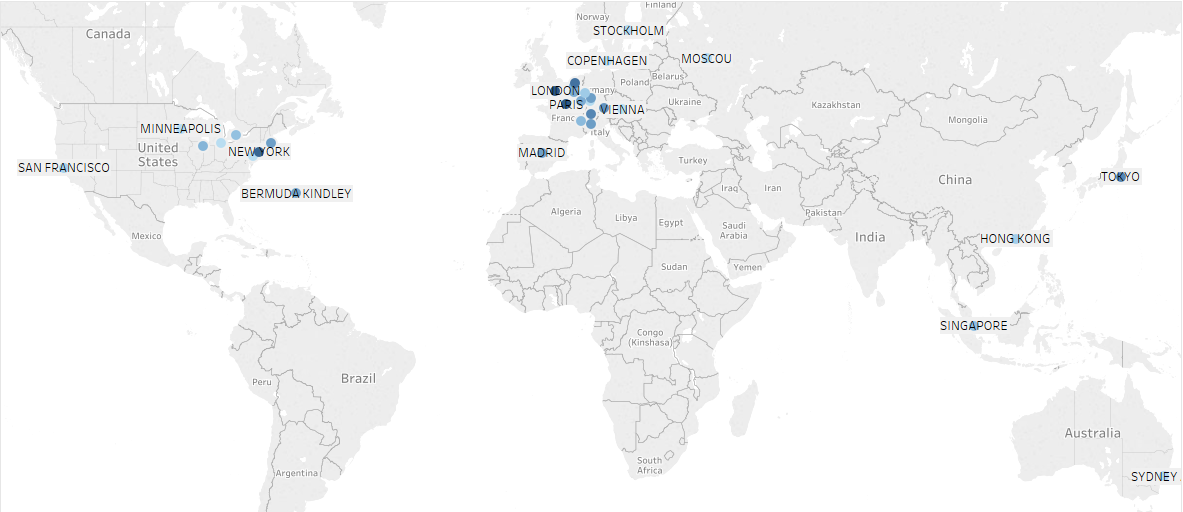
\includegraphics[width=1.0\linewidth]{city-networks-top-cumulative-map}
		\caption[Top economic cities on global map]{Top cities in the year 2010 and 2013 based on Cumulative Ranking.}
		\label{fig:city-networks-top-cumulative-map}
	\end{figure}
	
	\begin{figure}[ht]
		\centering
		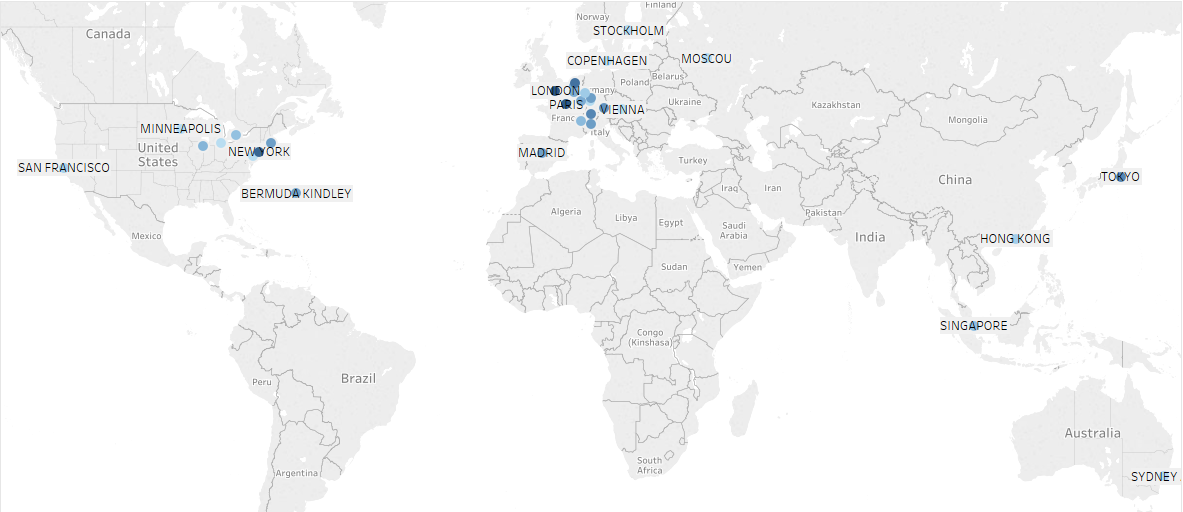
\includegraphics[width=1\linewidth]{city-networks-top-cumulative-map}
		\caption[Top economic cities with positive change on global map]{Top cities with positive change in cumulative rankings from 2010 to 2013.}
		\label{fig:city-networks-top-positive-cumulative-map}
	\end{figure}
	
	
	\begin{figure}[ht]
		\centering
		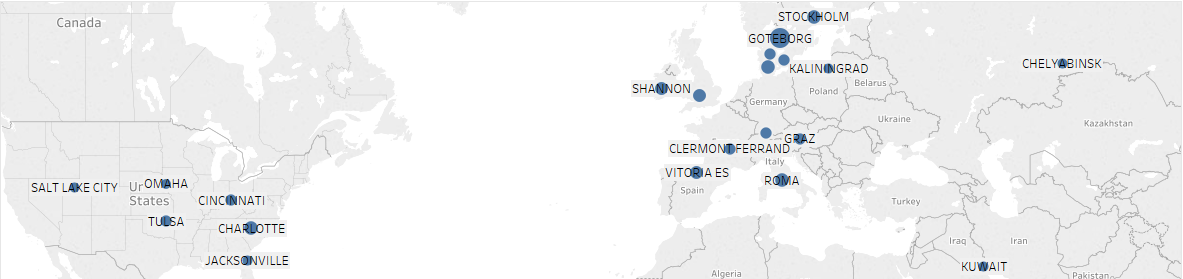
\includegraphics[width=1\linewidth]{city-networks-top-negative-cumulative-map}
		\caption[Top economic cities with negative change on global map]{Top cities with negative change in cumulative rankings from 2010 to 2013.}
		\label{fig:city-networks-top-negative-cumulative-map}
	\end{figure}

		\subsection{Supplementary comments}
		The cities with strongest development can be observed as spread out. In the Western Europe, we Mannheim and Haover from Germany, Jersey and Guernsey from the UK, Milan and Bologna from Italy, Antwerp from Belgium and Salzburg from Austria with positive growth. In the North American region, we see Kansas city, Tampa, Baltimore and Pheonix as good examples (in the US, these are not the top tier cities). On the East Asian front, we see that Beijing (China) is catching up with Hongkong, which outstripped Shanghai, the captal of China in economic and political movements. As for the Middle eastern Gulf region in Asia, Dubai and Abu Dhabi represent UAE and Cairo represents Egypt with all showing positive growth. There are some interesting observations as well, Akrotiri and Nicosia in Cyprus are outliers which might be developing due to Russian investments which transit into other European cities through these two. However, the intersting trend of developing nations showing strong growth continues as we see Rio De Jenario from Brazil, Istanbul from Turkey and Lagos fron Nigeria surfacing.
		
		In contrast, the declining cities which exhibit negative cumulative ranking appear mostly from USA, spread across East coast and central regions. Although most of these cities are not the strongest cities with respect to their presentation in multinational firms, we do see examples from Western Europe where traditionally strong economies lost their ranks. Friedrichshafen and Dortmund from Germany, Clermont-Ferrand and Annecy from France, Sonderborg and Copenhagen from Denmark, Goteborg and Stockholm from Sweden and Rome from Italy are such examples. Most interestingly, Kuwait City is an unexpected exception in this list.
		
		From these results, the most prominent findings we can draw are:
		
		\begin{enumerate}
			\item The cities which showed positive growth are spread across the world, contrary to common belief that the growth is concentrated only to some countries like China and Russia.
			
			\item The cities which were dominant in 2010 retaind their ranks in 2013 as well. The major change is mostly within the regions.
			
			\item Cities with highest decline in their ranks did not affect the globalization. They only lost their position within sub-regional system.
		\end{enumerate}
		
		The transformations we witness are within the regional sub-systems as highlighted by Rozenblat et. al. \cite{rozenblat2017}. Almost 3/4th of the ownerships of multinational links belong to North America, East Europe, Great Britain (alongside commonwealth countries), Japan, East Asia and India. The transformations do not change the regional dominance, but within the inner structure of regions. While we can clearly observe emergence of China and Middle East and declining trend in regions within US and Europe, some cities handled economic crisis comparatively better. This is also due to specialization functions of cities, some of which we enlist below:
		
		\begin{itemize}
			\item Swiss city Geneva is a highlight in finance domain with presence of most of the international banks and financial chains.
			
			\item Baltimore in USA, which has the highest positive change is a headquarter of high-tech industry.
			
			\item The island of Jersey, which is considered as a leading offshore financial city, is continually growing due to economic activity in financial sector.
			
			\item German city Mannheim, which showed positive growth is a well-known hub of medical technology innovations. The headquarters of several giants in medical tech, such as Siemens Healthcare and Roche Diagnostics are hosted in Mannheim. Another strong driving force causing the growth of Mannheim and some other German cities is the transport sector (Volkswagan).
			
			\item In Italy, Bolonga gains a spike due to boost in car manufacturing business. Ferrari, Ducati and Lamborghini to name a few manufacturers.
			
			\item Dubai, Abu Dhabi from UAE have diversified their economy in air transport, finance and technology. This diversification made them resilient to economic cisis and emerge as growing cities.
			
			\item Cairo (Egypt) and Lagos (Nigeria) are rising stars of Africa due to their integration with other global regions. Egpyt enjoys bounties from Suez canal and works as a bridge between Middle East and Africa.
			
		\end{itemize}
		
		The rise of Beijing and Shanghai, and the consecutive fall of Hongkong is no surprise. These reside in the same region and as foreseen, the disbalance occurs within the region more than external to it.
		
		The cities which declined steeply were due to some out of norm cause.For example, Swedish city Goteborg was hit by high unemployment due to its worst economic crisis in 2009; Ericsson and Volvo, the primary employers were the ones that faced the crisis the most. It only started recovering slowly from 2014, and is gaining its position back. Stockholm, the Swedish capital is another example which faced a drop during 2010 and 2013 after steady growth from 2008 to 2010. But from 2014 and onwards, we see Sweden's GDP to reflect a higher growth than most of regions in UK and Europe. Stockholm’s success stems from five major sectors, Trade in high-tech industries (refined petroleum products, electronics, chemicals, and transportation equipment), Innovation with a high number of patents with commercial and university-industry partnerships, Talent with highly educated work-force, Infrastructure (top quality freight, aviation, and broadband systems) and Governance which ensures that the policies support business success. Another examples comes from Denish city Sodenborg, which is a key player in heating and cooling products; this city is facing decline mainly due to overall decrease in GDP, as the growth in 2016 is reported to be 1.1\% only. In this case, the country's economy contributed to decline of city's economy.
	

	\section{The Influence Mining Framework}
	\label{sec:appendix-C-inf-framework}
	
	\begin{figure}[H]
		\begin{multicols}{2}
			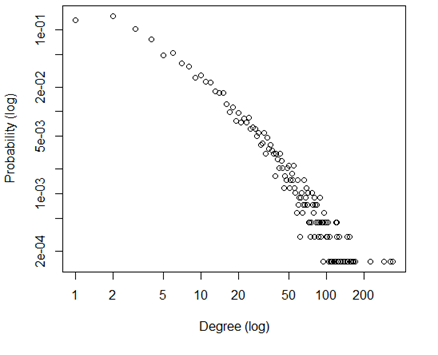
\includegraphics[width=\linewidth]{degree-distribution-arxiv}\par 
			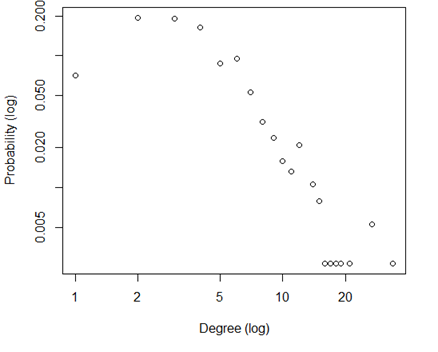
\includegraphics[width=\linewidth]{degree-distribution-author}\par 
		\end{multicols}
		\begin{multicols}{2}
			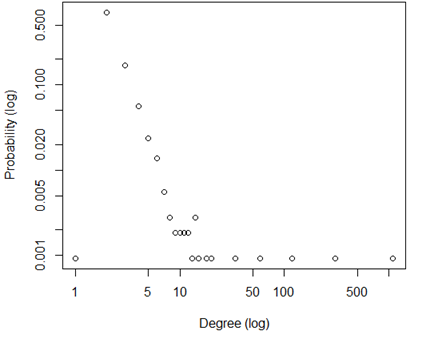
\includegraphics[width=\linewidth]{degree-distribution-automata}\par 
			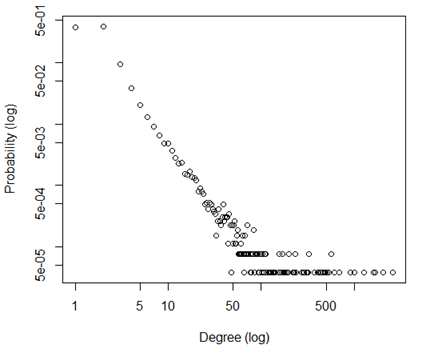
\includegraphics[width=\linewidth]{degree-distribution-caida}\par 
		\end{multicols}
		\begin{multicols}{2}
			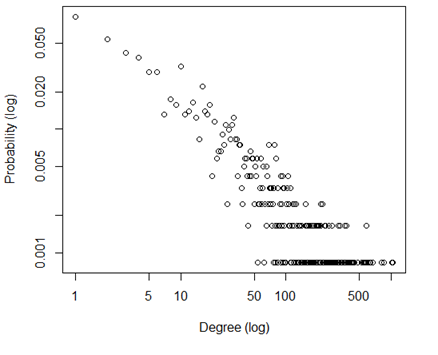
\includegraphics[width=\linewidth]{degree-distribution-city2010}\par 
			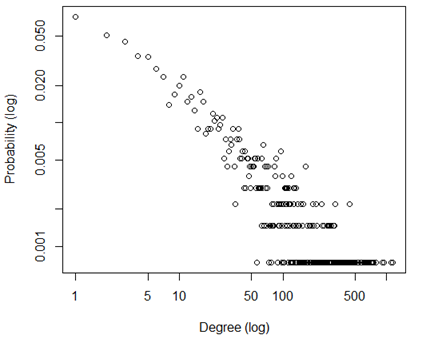
\includegraphics[width=\linewidth]{degree-distribution-city2013}\par 
		\end{multicols}
		\caption[Degree distribution log-log plots (1)]{Degree distribution log-log plots. ArXiv collaboration (arxiv) on Top-Left; Author NetScience (author) on Top-Right; Automata GraphDraw (automata) on Center-Left; AS-Caida (caida) on Center-Right; City Economic Networks (city2010) on Bottom-Left; City Economic Networks (city2013) on Bottom-Right}
		\label{fig:inf-framework-networks1}
	\end{figure}
	
	\begin{figure}[H]
		\begin{multicols}{2}
			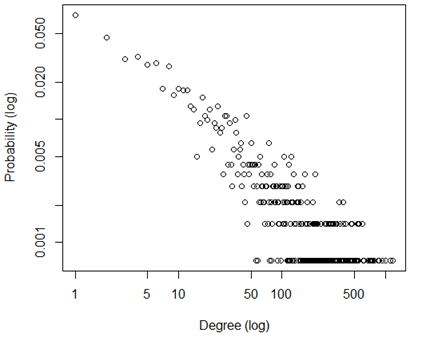
\includegraphics[width=\linewidth]{degree-distribution-city2016}\par 
			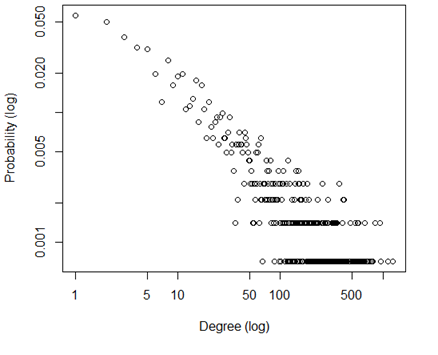
\includegraphics[width=\linewidth]{degree-distribution-city2019}\par 
		\end{multicols}
		\begin{multicols}{2}
			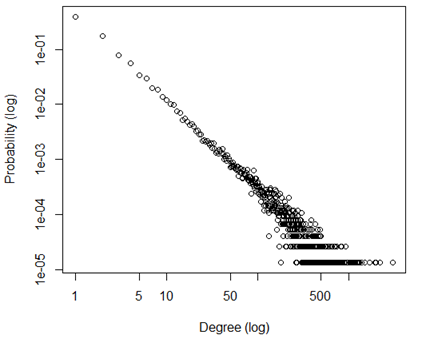
\includegraphics[width=\linewidth]{degree-distribution-epinions}\par 
			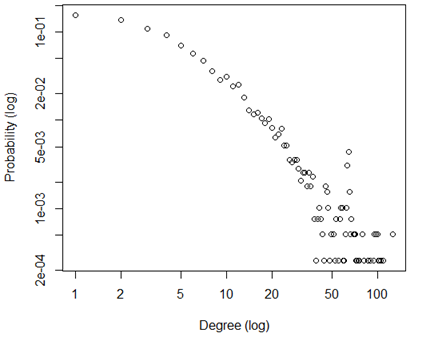
\includegraphics[width=\linewidth]{degree-distribution-fb_tvshows}\par 
		\end{multicols}
		\begin{multicols}{2}
			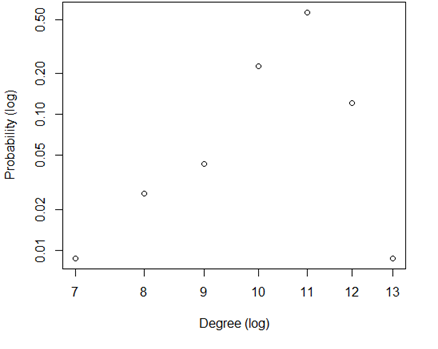
\includegraphics[width=\linewidth]{degree-distribution-football}\par 
			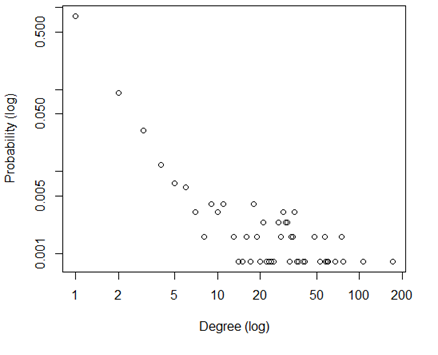
\includegraphics[width=\linewidth]{degree-distribution-influence_citation}\par 
		\end{multicols}
		\caption[Degree distribution log-log plots (2)]{City Economic Networks (city2016) on Top-Left; City Economic Networks (city2019) on Top-Right; Epinions.com (epinions) on Center-Left; Facebook TV shows (fb\_tvshows) on Center-Right; Football games (football) on Bottom-Left; Influence citations (influence\_citation) on Bottom-Right}
		\label{fig:inf-framework-networks2}
	\end{figure}
	
	\begin{figure}[H]
		\begin{multicols}{2}
			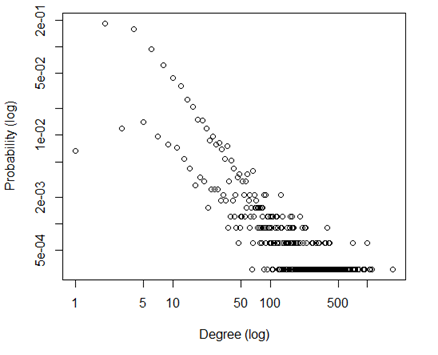
\includegraphics[width=\linewidth]{degree-distribution-ita2000}\par 
			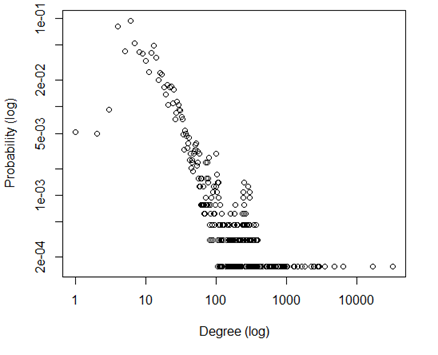
\includegraphics[width=\linewidth]{degree-distribution-jdk6}\par 
		\end{multicols}
		\begin{multicols}{2}
			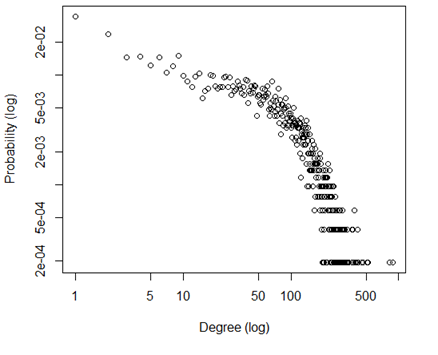
\includegraphics[width=\linewidth]{degree-distribution-johnshopkins}\par 
			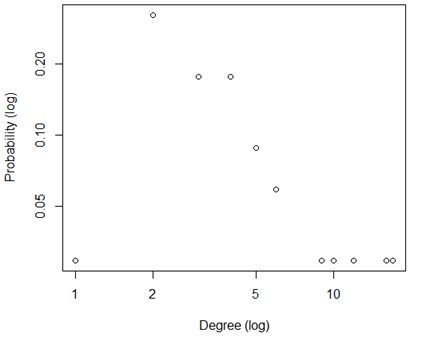
\includegraphics[width=\linewidth]{degree-distribution-karate}\par 
		\end{multicols}
		\begin{multicols}{2}
			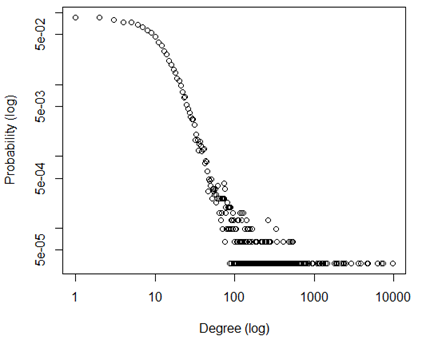
\includegraphics[width=\linewidth]{degree-distribution-linux}\par 
			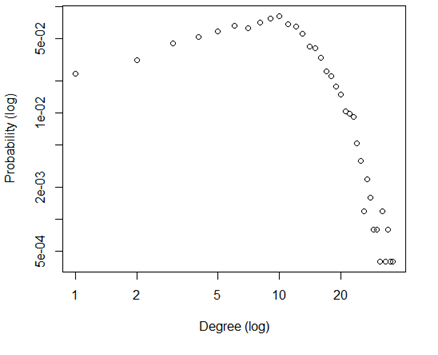
\includegraphics[width=\linewidth]{degree-distribution-moreno}\par 
		\end{multicols}
		\caption[Degree distribution log-log plots (3)]{ITA-2000 (ita2000) on Top-Left; Java Development Kit 6 Classes(jdk6) on Top-Right; Johns Hopkins University Facbook Network (johnshopkins) on Center-Left; Karate club (karate) on Center-Right; Linux source code (linux) on Bottom-Left; Moreno Student–student friendships (moreno) on Bottom-Right}
		\label{fig:inf-framework-networks3}
	\end{figure}
	
	\begin{figure}[H]
		\begin{multicols}{2}
			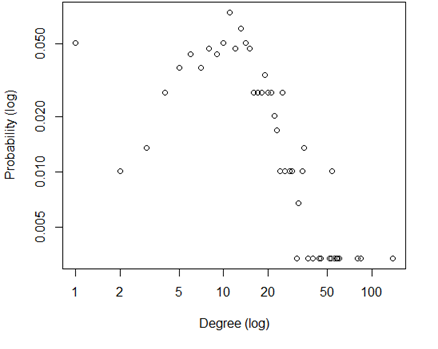
\includegraphics[width=\linewidth]{degree-distribution-nematode}\par 
			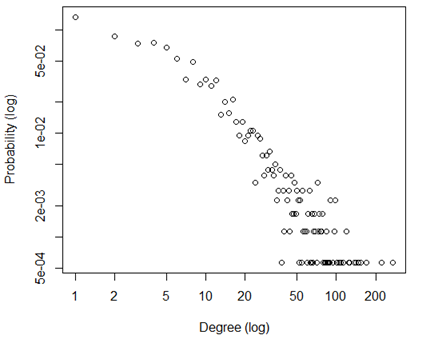
\includegraphics[width=\linewidth]{degree-distribution-hamster}\par 
		\end{multicols}
		\begin{multicols}{2}
			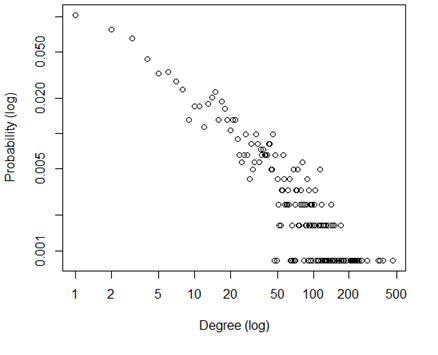
\includegraphics[width=\linewidth]{degree-distribution-political}\par 
			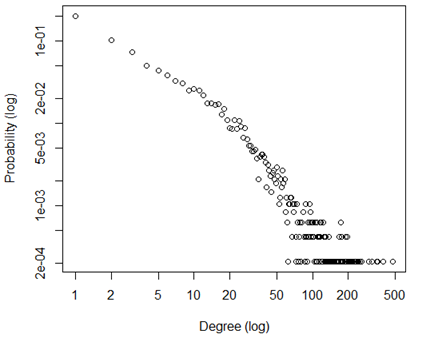
\includegraphics[width=\linewidth]{degree-distribution-spam}\par 
		\end{multicols}
		\begin{multicols}{2}
			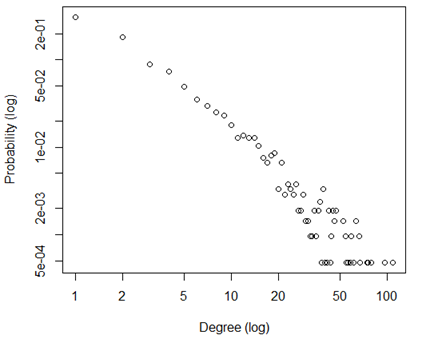
\includegraphics[width=\linewidth]{degree-distribution-routers}\par 
			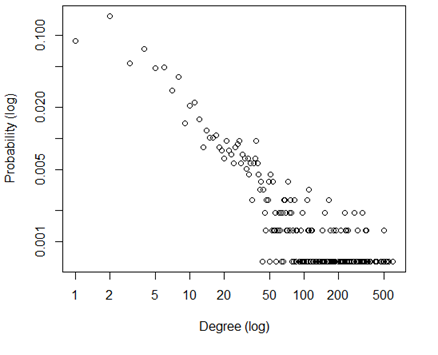
\includegraphics[width=\linewidth]{degree-distribution-usairport}\par 
		\end{multicols}
		\caption[Degree distribution log-log plots (4)]{Neural Network of Nematode (nematode) on Top-Left; Petster-hamster (hamster) on Top-Right; Political Blogs (political) on Center-Left; Spam on Web Challenge (spam) on Center-Right; Tech Routers(routers) on Bottom-Left; US Airport (usairport) on Bottom-Right}
		\label{fig:inf-framework-networks4}
	\end{figure}
	
	\begin{figure}[H]
		\begin{multicols}{2}
			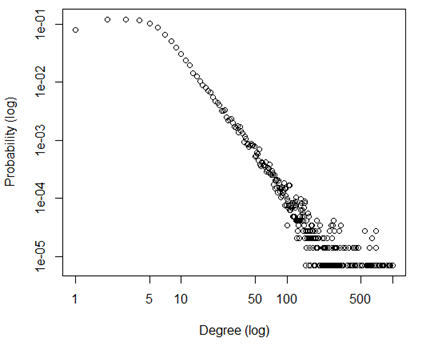
\includegraphics[width=\linewidth]{degree-distribution-wordnet}\par 
			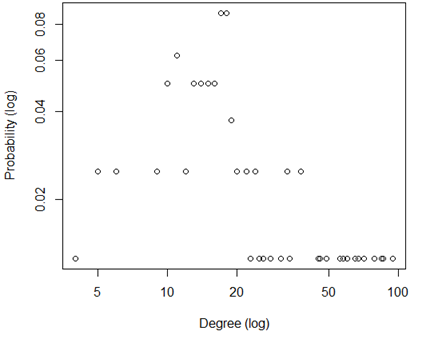
\includegraphics[width=\linewidth]{degree-distribution-world_trade}\par 
		\end{multicols}
		\begin{multicols}{1}
			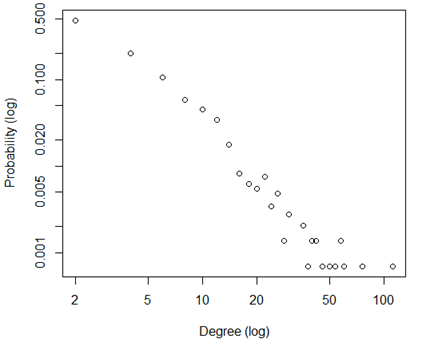
\includegraphics[width=\linewidth]{degree-distribution-protein}\par 
		\end{multicols}
		\caption[Degree distribution log-log plots (5)]{Word Net (wordnet) on Top-Left; World Trade (world\_trade) on Top-Right; Yeast Protein (protein) on Bottom-Left.}
		\label{fig:inf-framework-networks5}
	\end{figure}

		\subsection{Analysis of Dataset}
		\label{subsec:appendix-dataset-analysis}
		
		\begin{figure}[H]
			\centering
			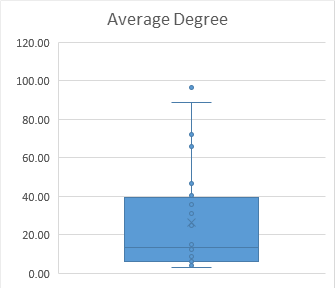
\includegraphics[width=0.7\textwidth]{inf-framework-networks-avg-degree}
			\caption{Boxplot of average degrees of the networks.}
			\label{fig:inf-framework-networks-avg-degree}
		\end{figure}
		
		\begin{figure}[H]
			\centering
			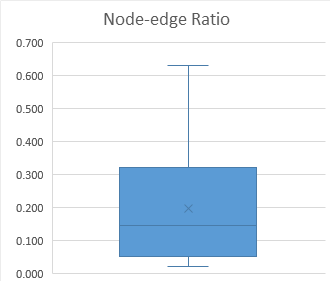
\includegraphics[width=0.7\textwidth]{inf-framework-networks-ratio}
			\caption{Boxplot of Node-edge ratios of the networks.}
			\label{fig:inf-framework-networks-ratio}
		\end{figure}
		
		\begin{figure}[H]
			\centering
			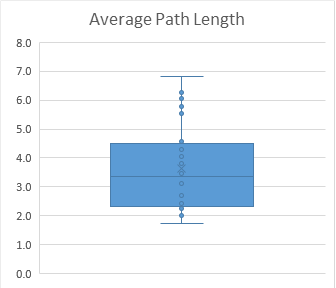
\includegraphics[width=0.7\textwidth]{inf-framework-networks-apl}
			\caption{Boxplot of Average Path Lengths of the networks.}
			\label{fig:inf-framework-networks-apl}
		\end{figure}
		
		\begin{figure}[H]
			\centering
			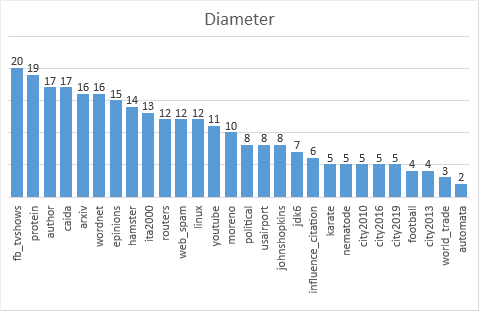
\includegraphics[width=0.7\textwidth]{inf-framework-networks-diameter}
			\caption{Diameters of the networks in descending order.}
			\label{fig:inf-framework-networks-diameter}
		\end{figure}
		
		On transitivity, only fb\_tvshows has an unusually high value of transitivity (0.59), the networks are majorly ranging between 0.15 and 0.35 (see Figure \ref{fig:inf-framework-networks-transitivity}). The higher value means tighter clique-like structure.
		
		\begin{figure}[H]
			\centering
			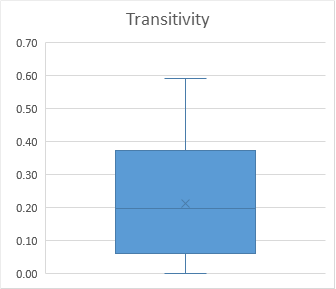
\includegraphics[width=0.7\textwidth]{inf-framework-networks-transitivity}
			\caption{Boxplot of Transitivity of the networks.}
			\label{fig:inf-framework-networks-transitivity}
		\end{figure}
		
		Assortativity is a unique metric which is used to understand dynamic properties of a graph, for example against a targeted attack a highly assortative network will be infected completely differently than a low assortative network. We note that the data set covers a wide spectrum of networks with a few highly assortative, few highly disassortative, and several low assortative/disassortative networks; this is shown in histogram \ref{fig:inf-framework-networks-assortativity}.
		
		\begin{figure}[H]
			\centering
			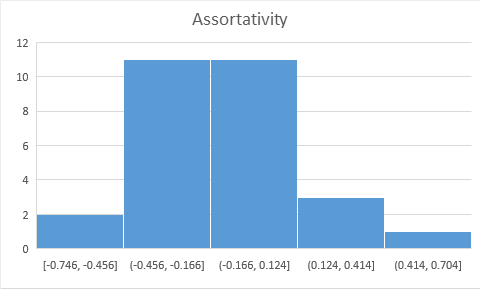
\includegraphics[width=0.7\textwidth]{inf-framework-networks-assortativity}
			\caption{Histogram of Assortativity of the networks.}
			\label{fig:inf-framework-networks-assortativity}
		\end{figure}
		
		Looking at the power-law, the minimum, mean, maximum and outlier values are 1.69, 3.23, 8.42, 21.19 respectively. Thus indicating that most of the networks follow power-law distribution. All the distribution plots %todo distribution plots of what? degree? 
		can be found in Appendix \ref{sec:appendix-C-inf-framework}.
		
		In a nutshell, the selection of networks ensures that the results will not be biased by networks with any specific structure. %and focus on only one or two types of complex networks.

		\subsection{Evaluation results of IMine framework}
		\label{subsec:appendix-imine-evaluation}
		
		\begin{figure}[H]
			\centering
			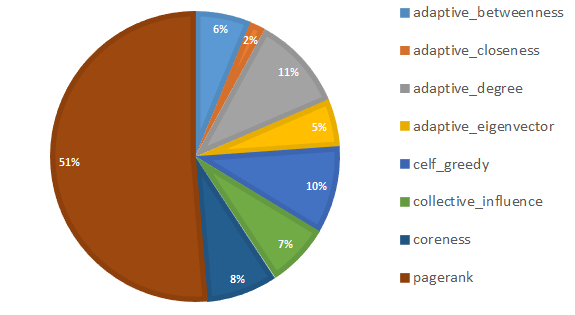
\includegraphics[width=0.75\textwidth]{inf-summary-budget-influence-ic}
			\caption[IMine performance on budget criteria for Influence\_IC test]{Percentage of number of instances each method outperformed the other methods for INFLUENCE\_IC test in budget criteria. The method with highest influence was selected as the best method. Pagerank ranked top (51\%), followed by CELF-greedy (10\%), while Adaptive Closeness performed worst (2\%).}
			\label{fig:inf-summary-budget-influence-ic}
		\end{figure}
		
		\begin{figure}[H]
			\centering
			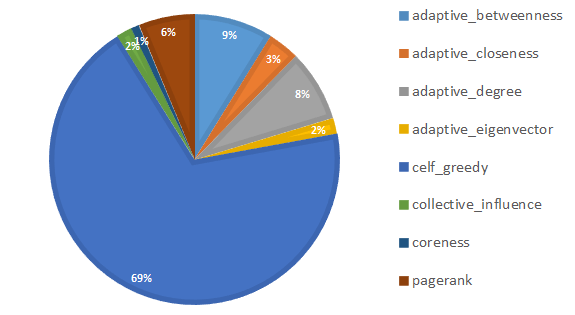
\includegraphics[width=0.75\textwidth]{inf-summary-budget-influence-lt}
			\caption[IMine performance on budget criteria for Influence\_LT test]{Percentage of number of instances each method outperformed the other methods for INFLUENCE\_LT test in budget criteria. The method with most highest was selected as the best method. As clearly shown, CELF-greedy outperformed all other methods by a wide margin (69\%), where Coreness performed poorer than all (1\%).}
			\label{fig:inf-summary-budget-influence-lt}
		\end{figure}
		
		\begin{figure}[H]
			\centering
			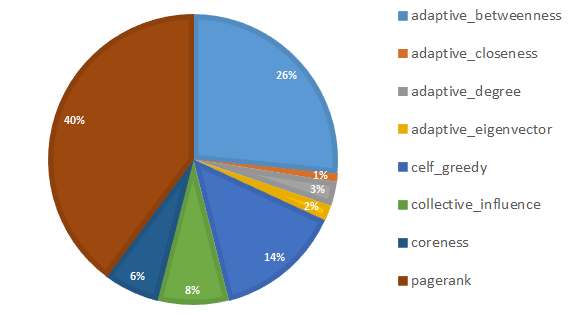
\includegraphics[width=1\textwidth]{inf-summary-budget-resilience}
			\caption[IMine performance on budget criteria for Resilience test]{Percentage of number of instances each method outperformed the other methods for RESILIENCE test in budget criteria. The method with most highest was selected as the best method. Pagerank turned out to be top performer in the trails (40\%), followed by Adaptive Betweenness (26\%), where Adaptive Closeness ranked last (1\%).}
			\label{fig:inf-summary-budget-resilience}
		\end{figure}
		
		\begin{figure}[H]
			\centering
			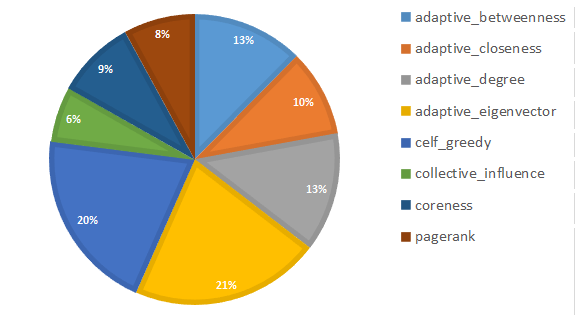
\includegraphics[width=1\textwidth]{inf-summary-influence-influence-ic}
			\caption[IMine performance on influence criteria for Influence\_IC test]{Percentage of number of instances each method outperformed the other methods for INFLUENCE\_IC test in influence criteria. The method with most highest was selected as the best method. }
			\label{fig:inf-summary-influence-influence-ic}
		\end{figure}
		
		\begin{figure}[H]
			\centering
			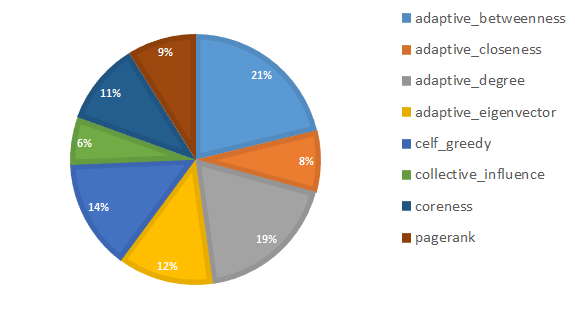
\includegraphics[width=1\textwidth]{inf-summary-influence-influence-lt}
			\caption[IMine performance on influence criteria for Influence\_LT test]{Percentage of number of instances each method outperformed the other methods for INFLUENCE\_LT test in influence criteria. The method with most highest was selected as the best method.}
			\label{fig:inf-summary-influence-influence-lt}
		\end{figure}
		
		\begin{figure}[H]
			\centering
			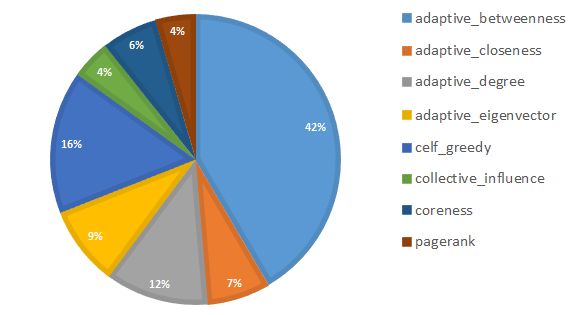
\includegraphics[width=1\textwidth]{inf-summary-influence-resilience}
			\caption[IMine performance on budget criteria for Resilience test]{Percentage of number of instances each method outperformed the other methods for RESILIENCE test in influence criteria. The method with most highest was selected as the best method.}
			\label{fig:inf-summary-influence-resilience}
		\end{figure}
		
		
		% *** arxiv ***
		\begin{figure*}[ht]
			\begin{multicols}{2}
				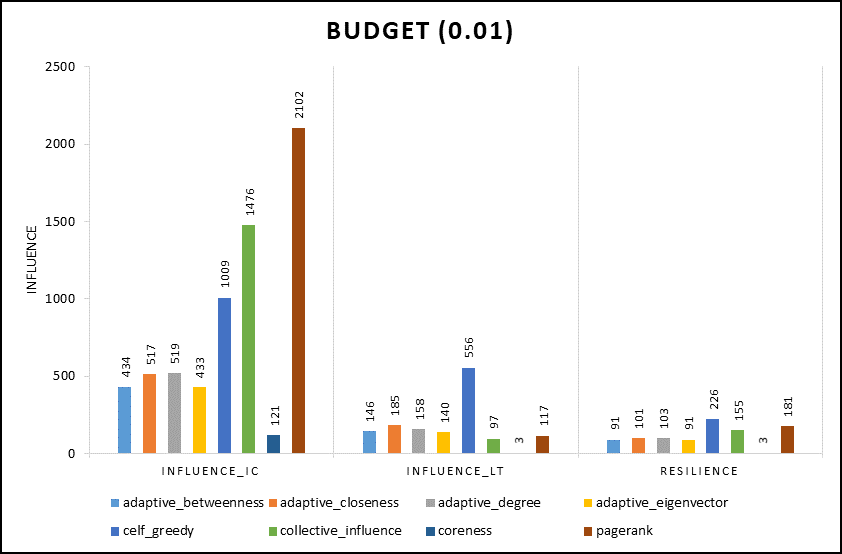
\includegraphics[angle=90, scale=0.65]{arxiv-budget-1}\par 
				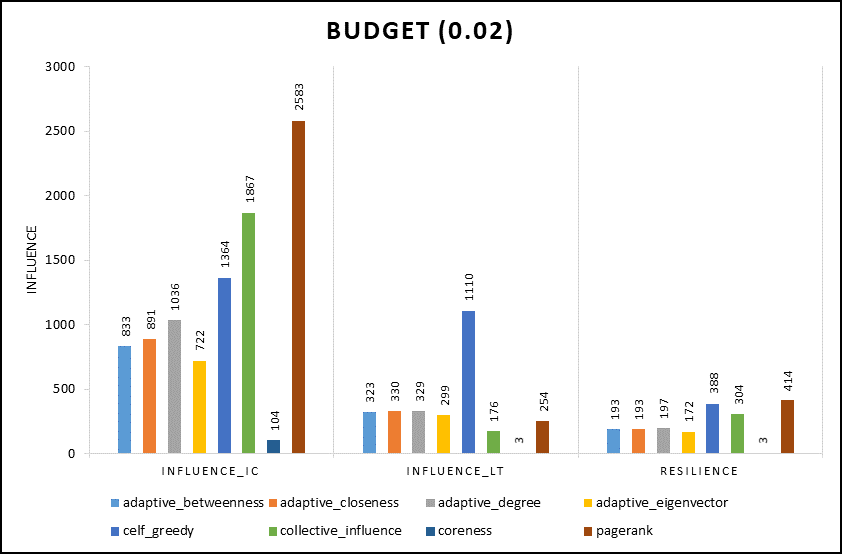
\includegraphics[angle=90, scale=0.65]{arxiv-budget-2}\par 
			\end{multicols}
			\begin{multicols}{2}
				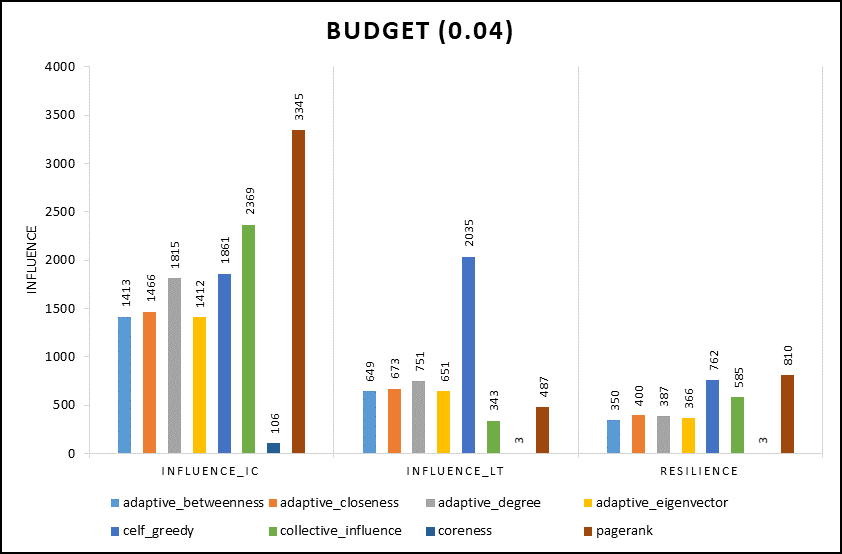
\includegraphics[angle=90, scale=0.65]{arxiv-budget-4}\par 
				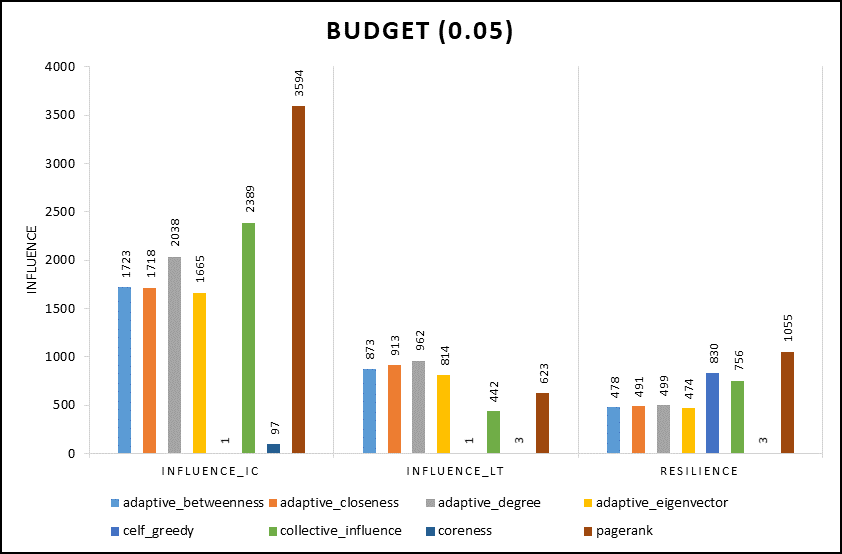
\includegraphics[angle=90, scale=0.65]{arxiv-budget-5}\par 
			\end{multicols}
			
			\caption{Influence measure of Arxiv network on range on all budgets evaluated for all three tests.}
			\label{fig:inf-framework-arxiv}
		\end{figure*}
		
		\begin{figure*}[ht]
			\begin{multicols}{2}
				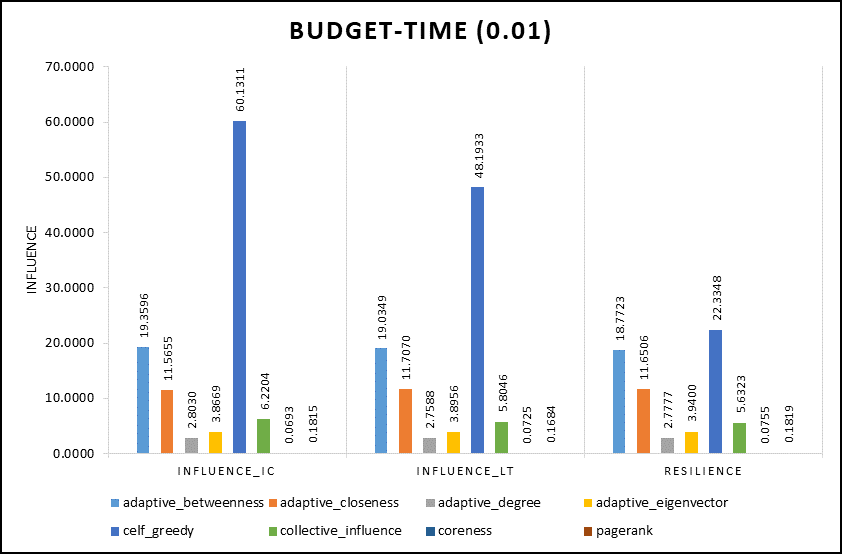
\includegraphics[angle=90, scale=0.65]{arxiv-budget-time-1}\par 
				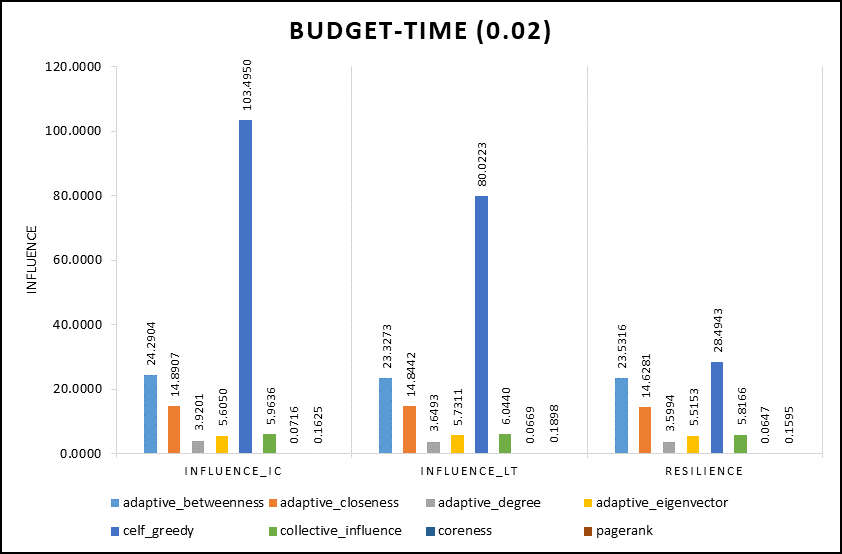
\includegraphics[angle=90, scale=0.65]{arxiv-budget-time-2}\par 
			\end{multicols}
			\begin{multicols}{2}
				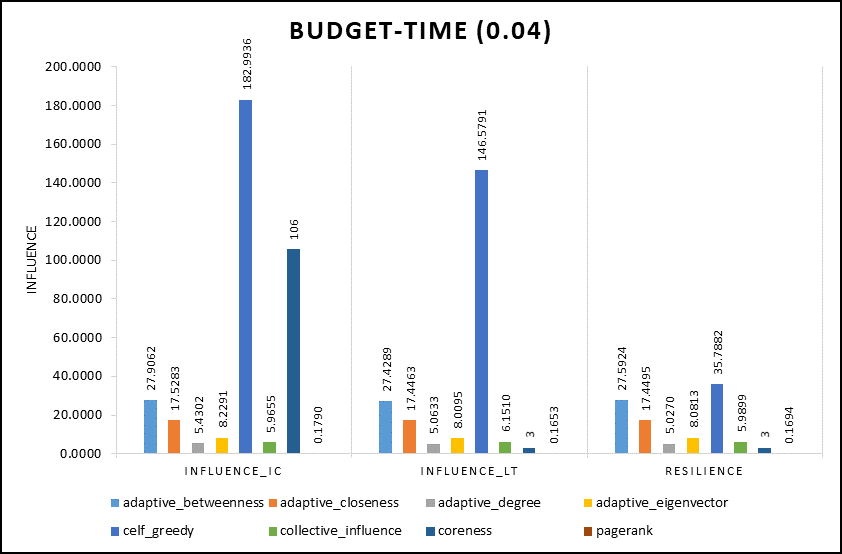
\includegraphics[angle=90, scale=0.65]{arxiv-budget-time-4}\par 
				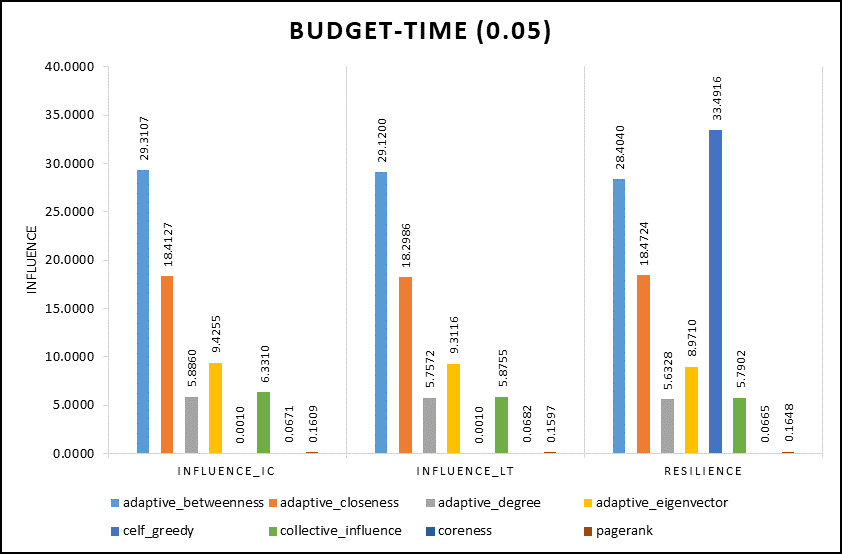
\includegraphics[angle=90, scale=0.65]{arxiv-budget-time-5}\par 
			\end{multicols}
			
			\caption{Normalized elapsed time for budget criteria on Arxiv network.}
			\label{fig:inf-framework-arxiv2}
		\end{figure*}
		
		\begin{figure*}[h]
			\begin{multicols}{2}
				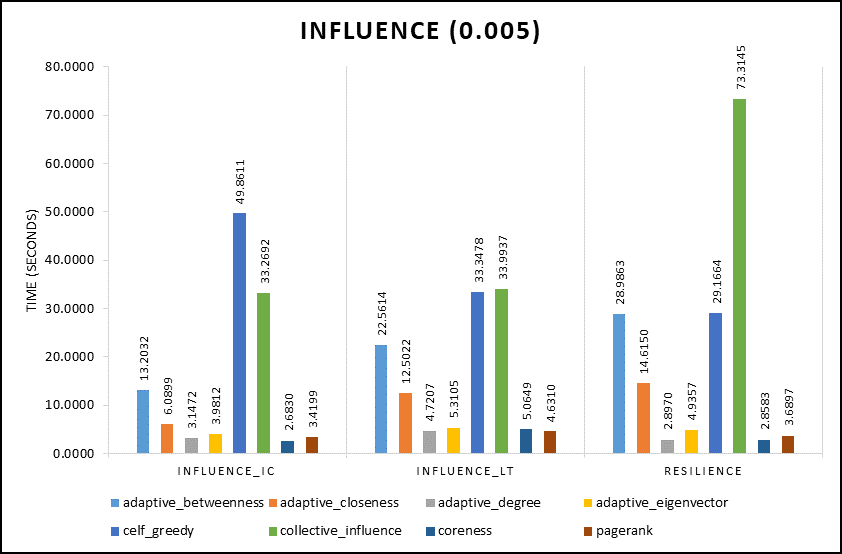
\includegraphics[angle=90, scale=0.65]{arxiv-influence-1}\par 
				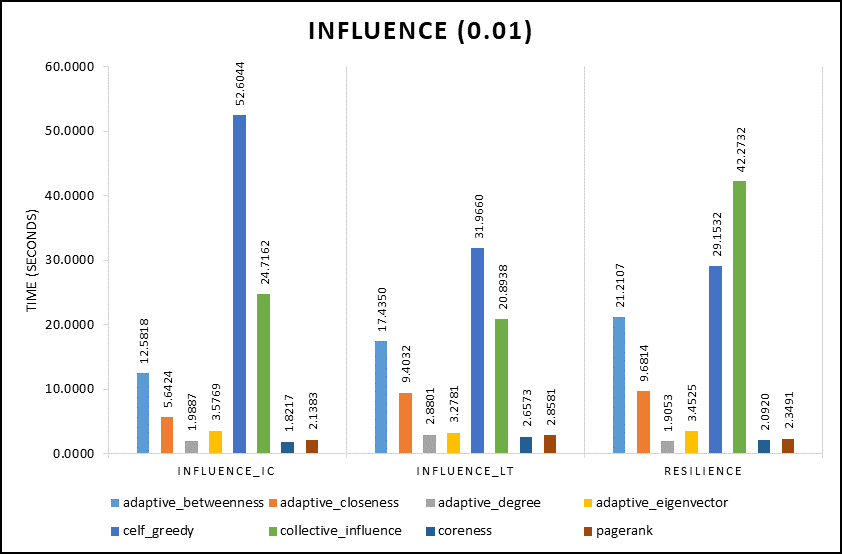
\includegraphics[angle=90, scale=0.65]{arxiv-influence-2}\par 
			\end{multicols}
			\begin{multicols}{2}
				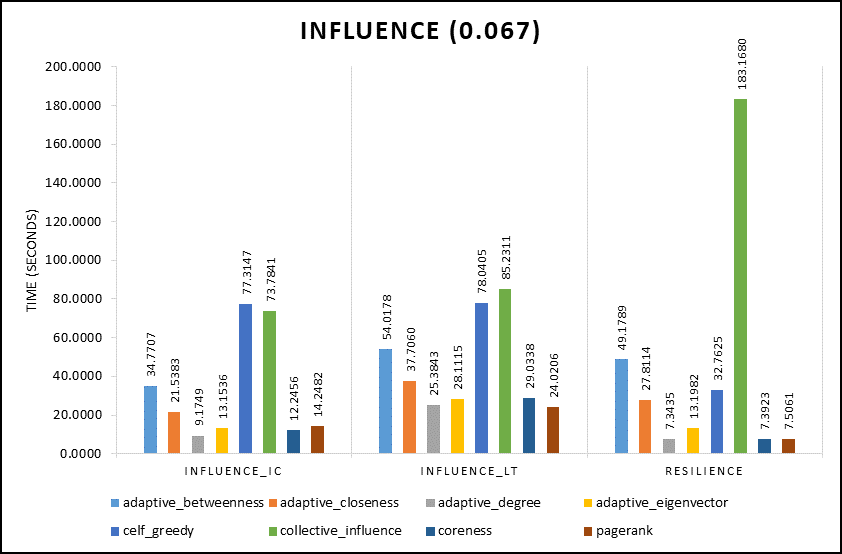
\includegraphics[angle=90, scale=0.65]{arxiv-influence-4}\par 
				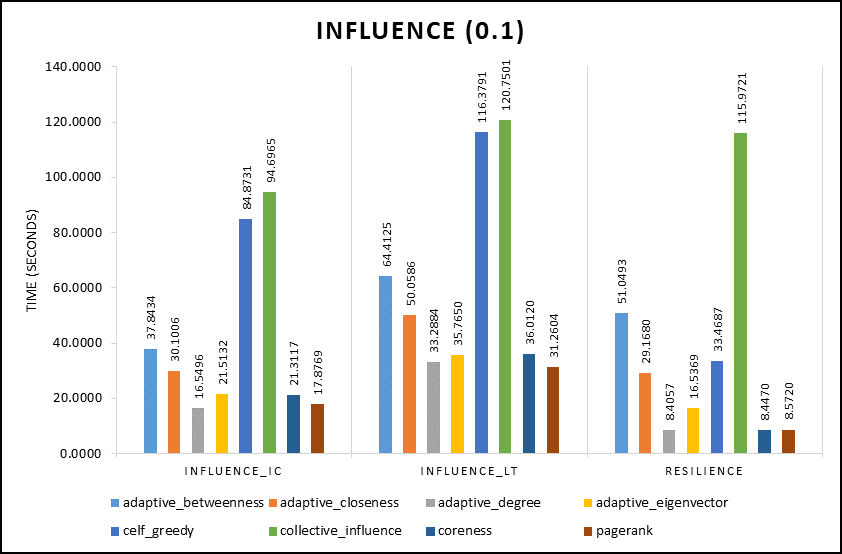
\includegraphics[angle=90, scale=0.65]{arxiv-influence-5}\par 
			\end{multicols}
			
			\caption{Normalized elapsed time for influence criteria on Arxiv network.}
			\label{fig:inf-framework-arxiv3}
		\end{figure*}
		
		
		% *** author ***
		\begin{figure*}[ht]
			\begin{multicols}{2}
				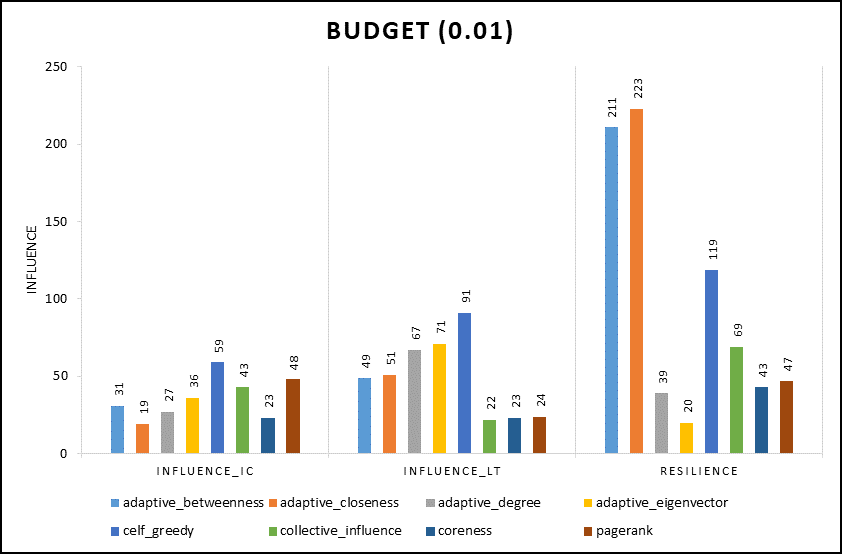
\includegraphics[angle=90, scale=0.65]{author-budget-1}\par 
				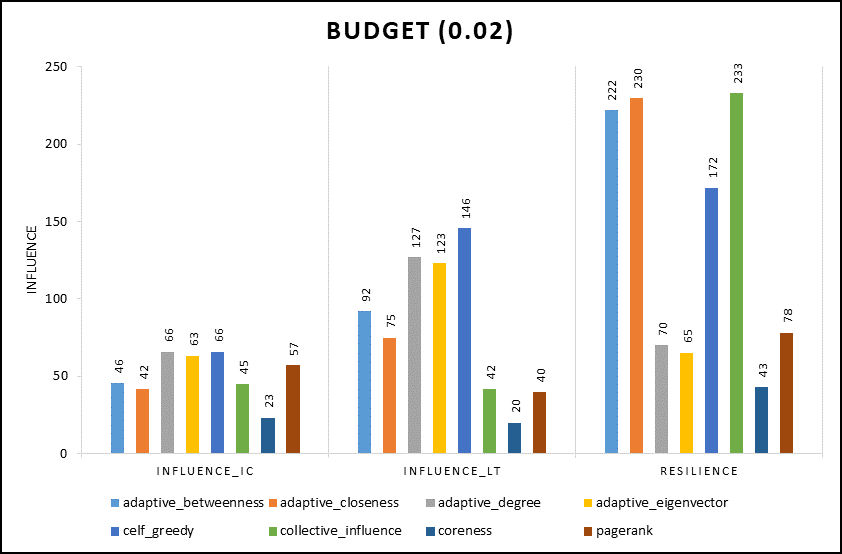
\includegraphics[angle=90, scale=0.65]{author-budget-2}\par 
			\end{multicols}
			\begin{multicols}{2}
				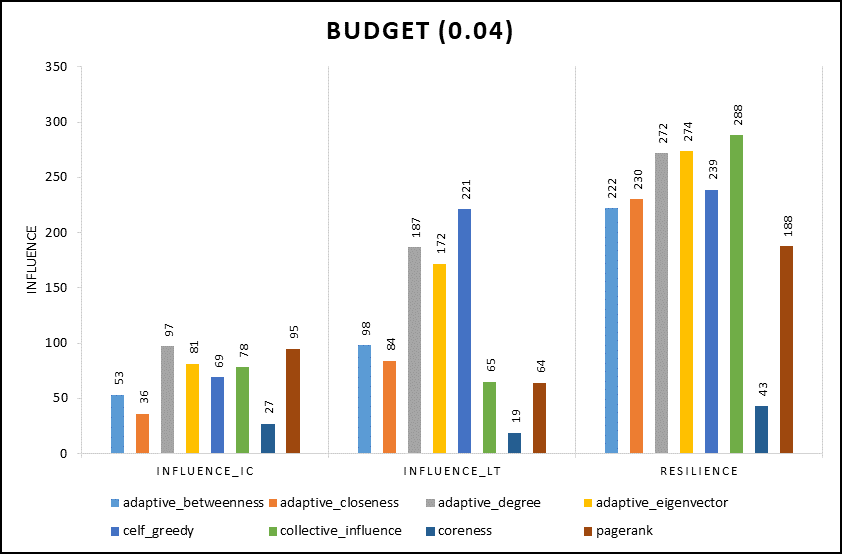
\includegraphics[angle=90, scale=0.65]{author-budget-4}\par 
				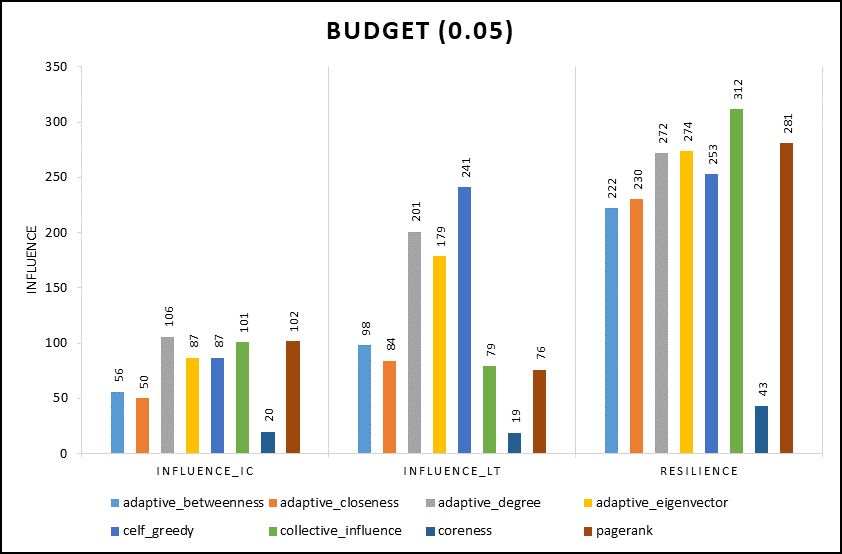
\includegraphics[angle=90, scale=0.65]{author-budget-5}\par 
			\end{multicols}
			
			\caption{Influence measure of Co-authorship network on range on all budgets evaluated for all three tests.}
			\label{fig:inf-framework-author}
		\end{figure*}
		
		\begin{figure*}[ht]
			\begin{multicols}{2}
				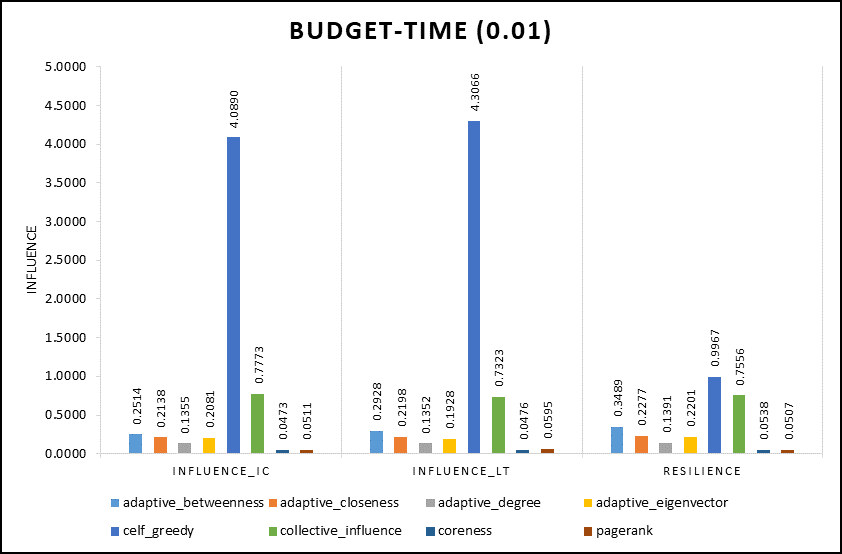
\includegraphics[angle=90, scale=0.65]{author-budget-time-1}\par 
				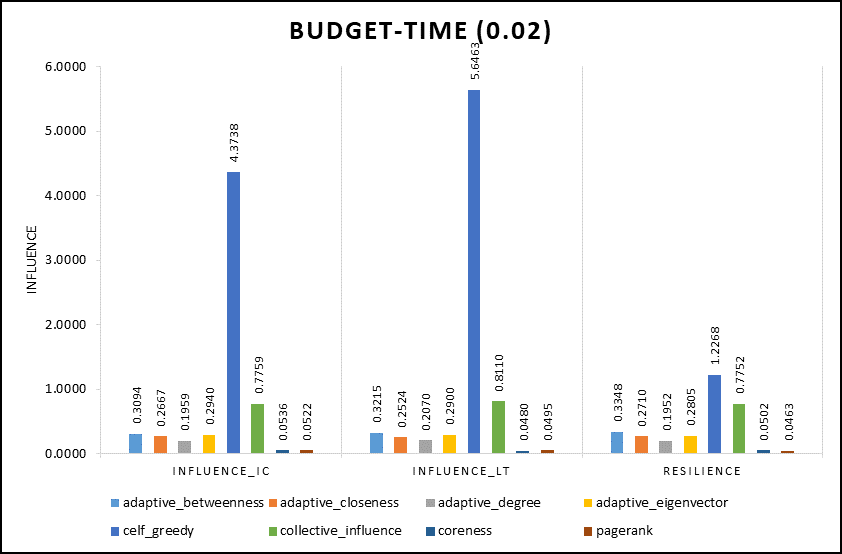
\includegraphics[angle=90, scale=0.65]{author-budget-time-2}\par 
			\end{multicols}
			\begin{multicols}{2}
				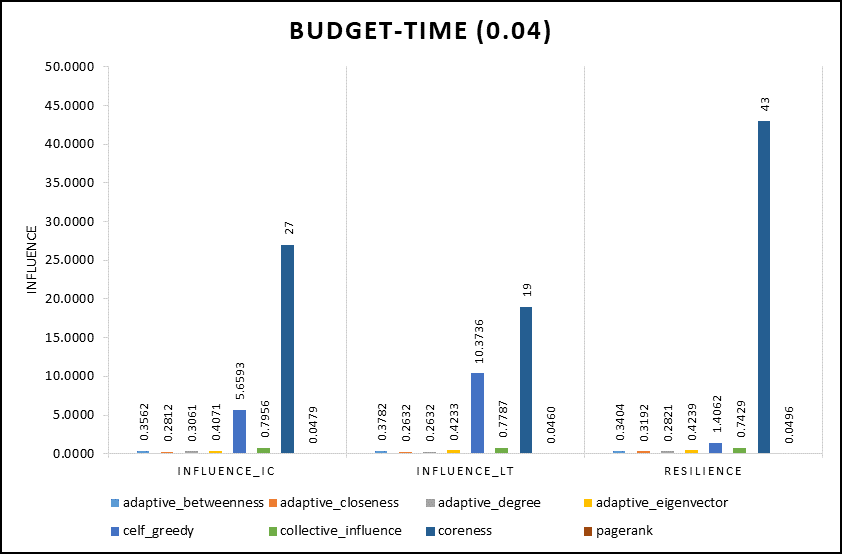
\includegraphics[angle=90, scale=0.65]{author-budget-time-4}\par 
				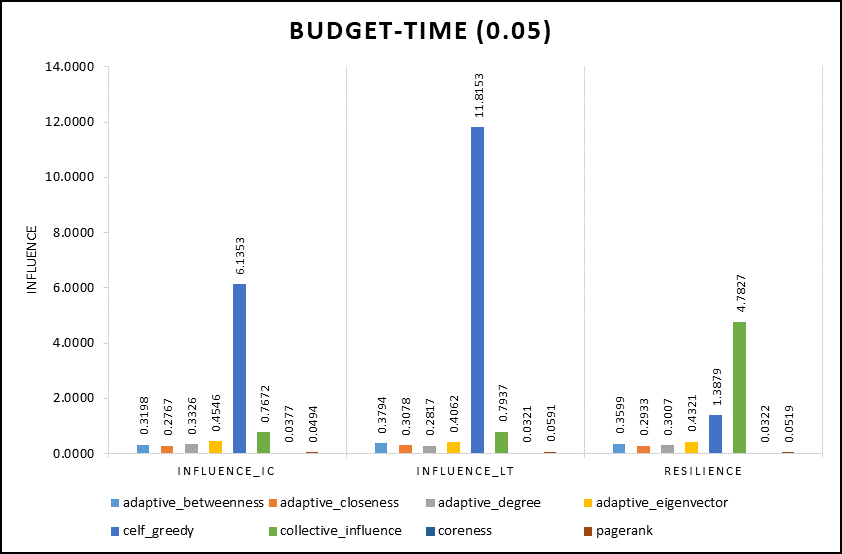
\includegraphics[angle=90, scale=0.65]{author-budget-time-5}\par 
			\end{multicols}
			
			\caption{Normalized elapsed time for budget criteria on Co-authorship network.}
			\label{fig:inf-framework-author2}
		\end{figure*}
		
		\begin{figure*}[h]
			\begin{multicols}{2}
				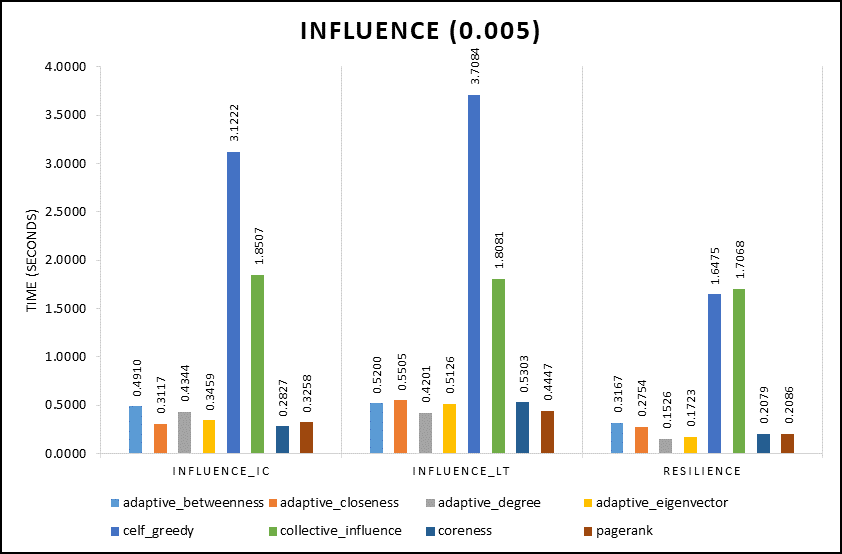
\includegraphics[angle=90, scale=0.65]{author-influence-1}\par 
				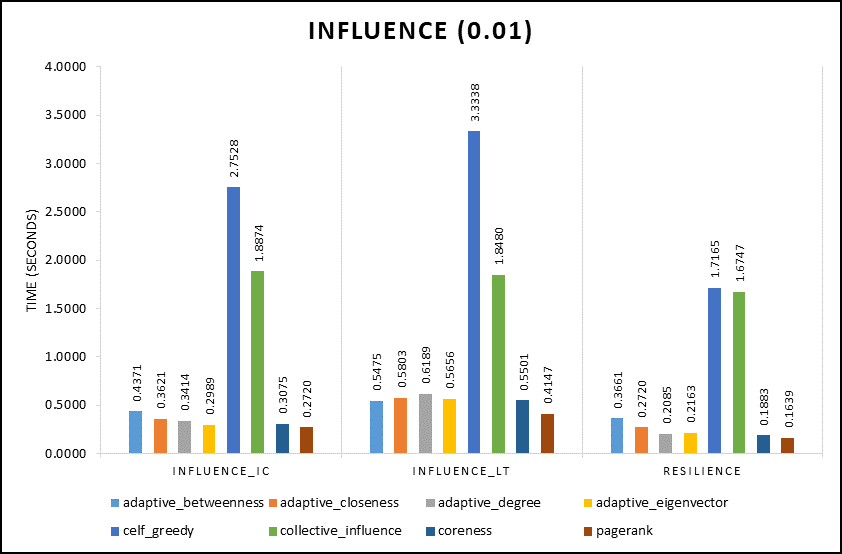
\includegraphics[angle=90, scale=0.65]{author-influence-2}\par 
			\end{multicols}
			\begin{multicols}{2}
				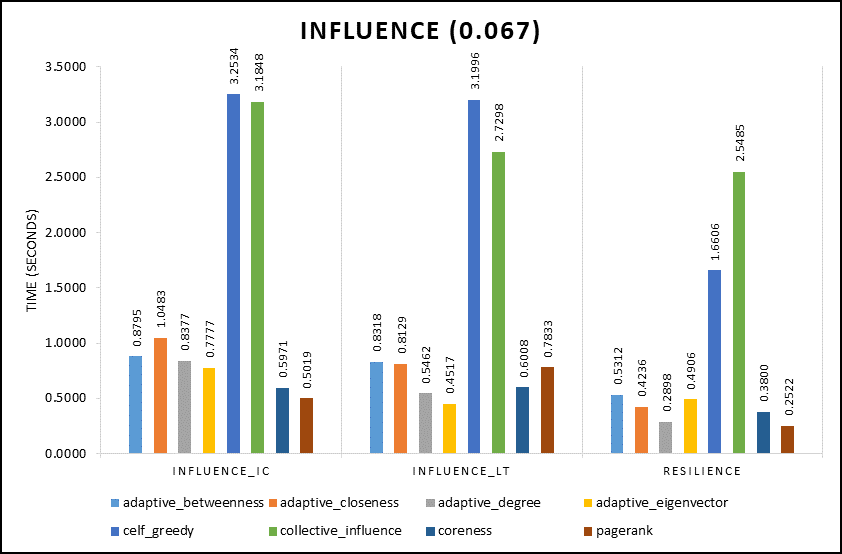
\includegraphics[angle=90, scale=0.65]{author-influence-4}\par 
				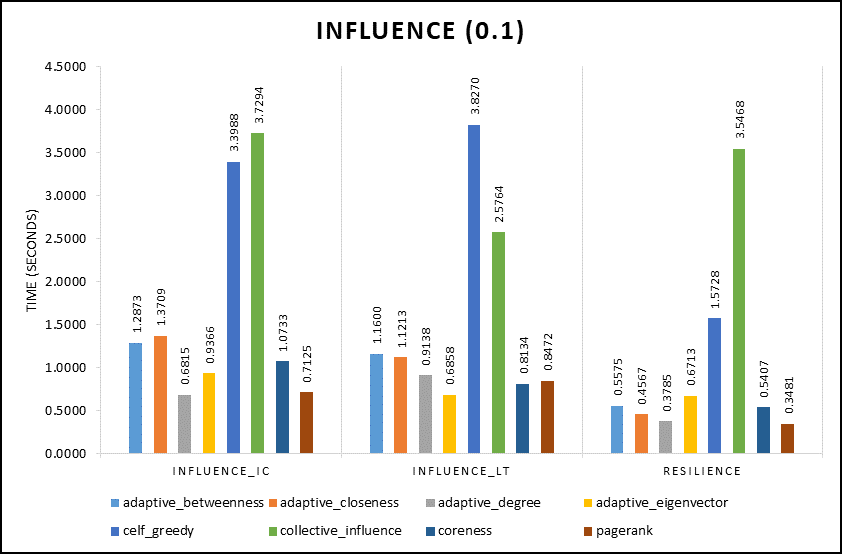
\includegraphics[angle=90, scale=0.65]{author-influence-5}\par 
			\end{multicols}
			
			\caption{Normalized elapsed time for influence criteria on Co-authorship network.}
			\label{fig:inf-framework-author3}
		\end{figure*}
		
		
		% *** automata ***
		\begin{figure*}[ht]
			\begin{multicols}{2}
				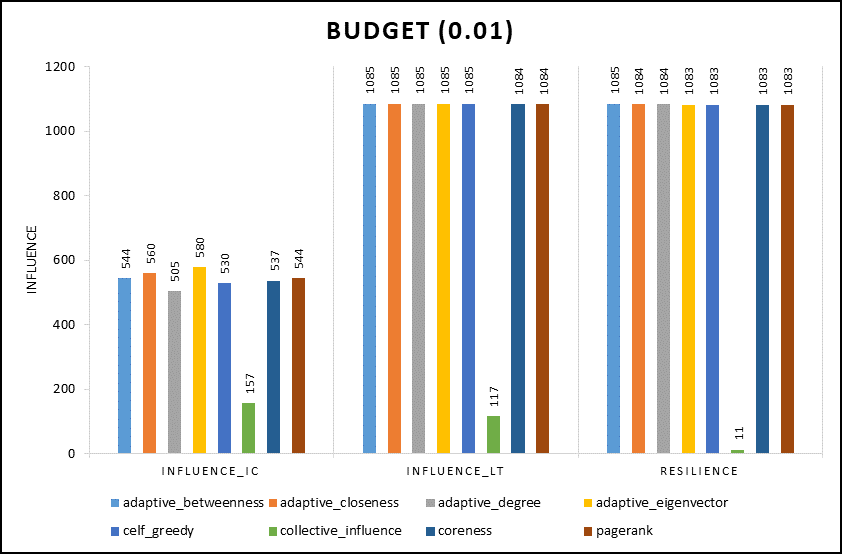
\includegraphics[angle=90, scale=0.65]{automata-budget-1}\par 
				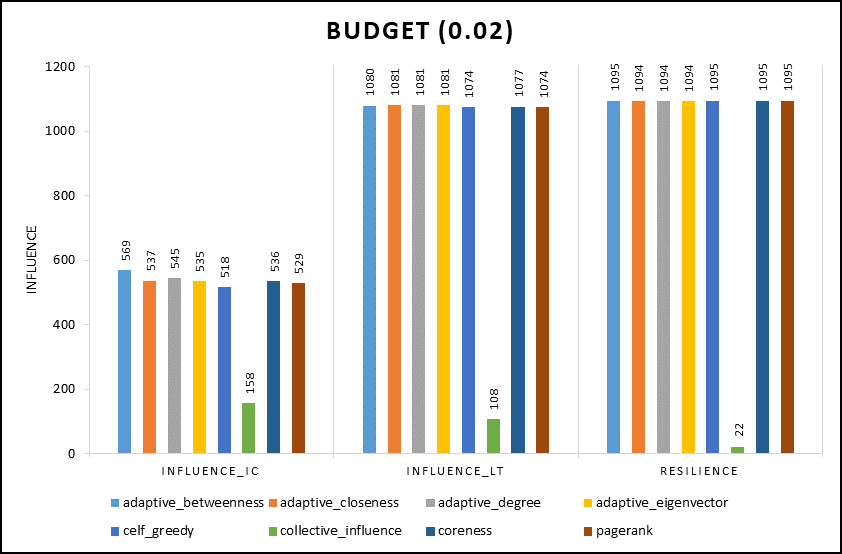
\includegraphics[angle=90, scale=0.65]{automata-budget-2}\par 
			\end{multicols}
			\begin{multicols}{2}
				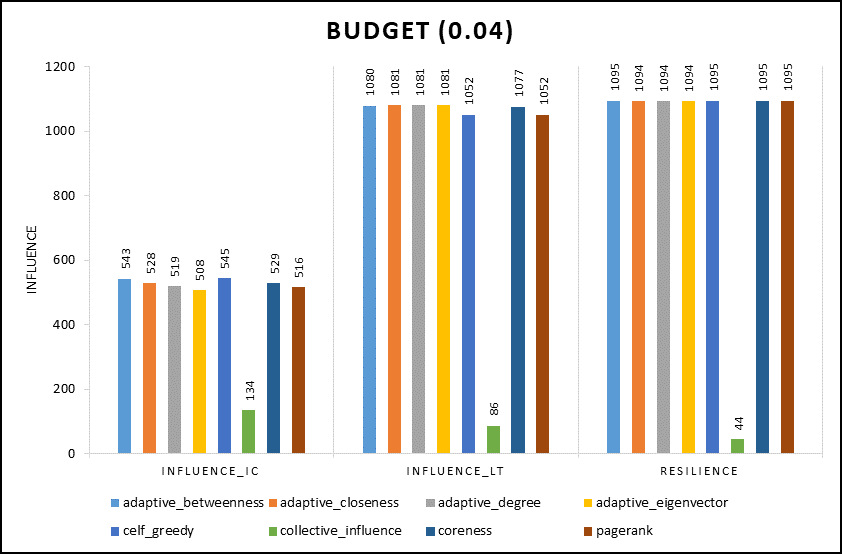
\includegraphics[angle=90, scale=0.65]{automata-budget-4}\par 
				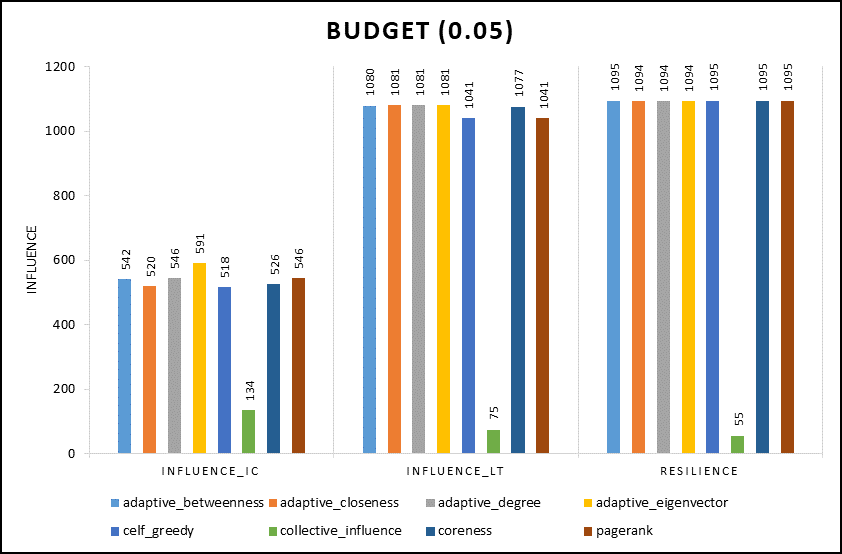
\includegraphics[angle=90, scale=0.65]{automata-budget-5}\par 
			\end{multicols}
			
			\caption{Influence measure of Automata network on range on all budgets evaluated for all three tests.}
			\label{fig:inf-framework-automata}
		\end{figure*}
		
		\begin{figure*}[ht]
			\begin{multicols}{2}
				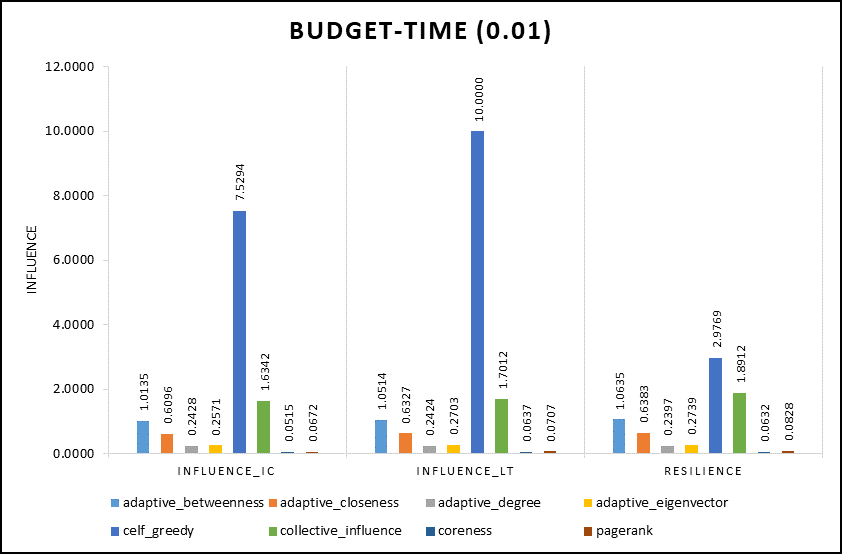
\includegraphics[angle=90, scale=0.65]{automata-budget-time-1}\par 
				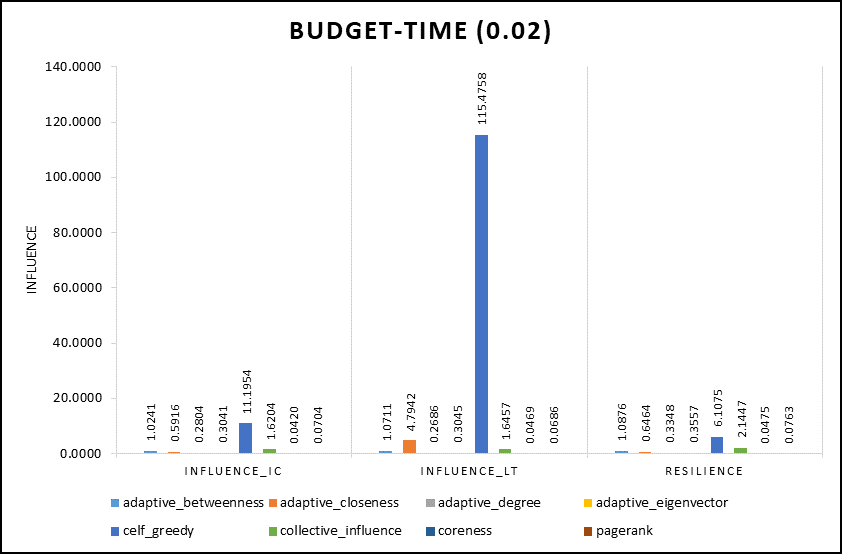
\includegraphics[angle=90, scale=0.65]{automata-budget-time-2}\par 
			\end{multicols}
			\begin{multicols}{2}
				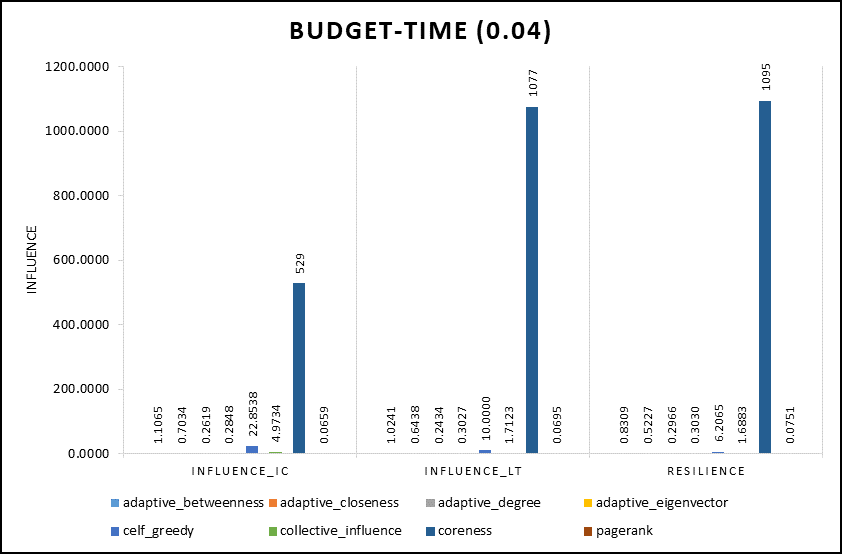
\includegraphics[angle=90, scale=0.65]{automata-budget-time-4}\par 
				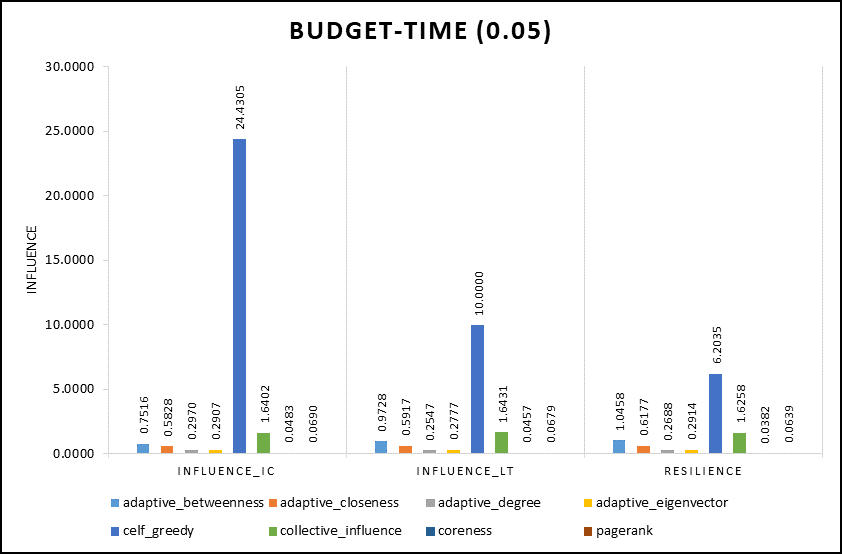
\includegraphics[angle=90, scale=0.65]{automata-budget-time-5}\par 
			\end{multicols}
			
			\caption{Normalized elapsed time for budget criteria on Automata network.}
			\label{fig:inf-framework-automata2}
		\end{figure*}
		
		\begin{figure*}[h]
			\begin{multicols}{2}
				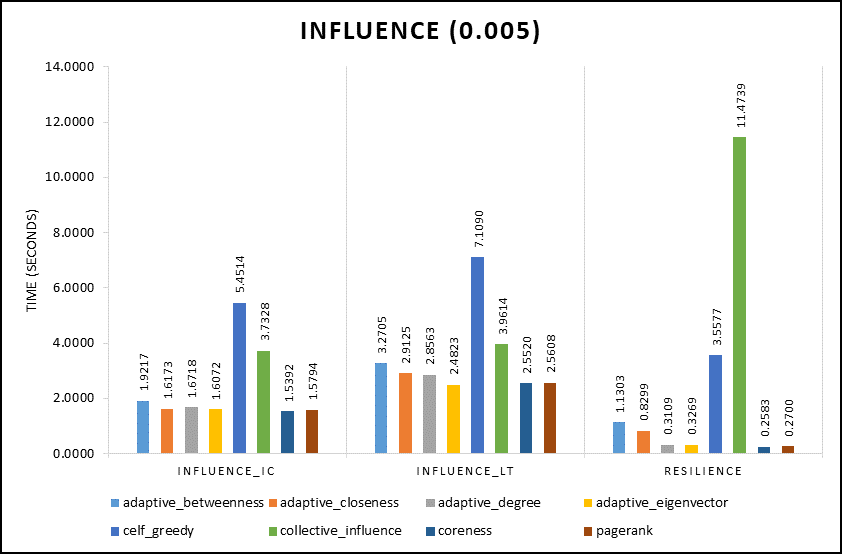
\includegraphics[angle=90, scale=0.65]{automata-influence-1}\par 
				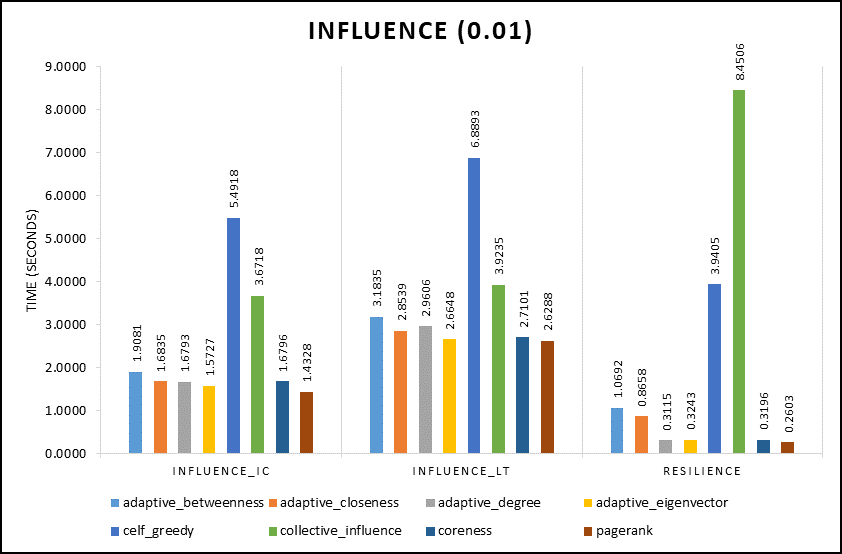
\includegraphics[angle=90, scale=0.65]{automata-influence-2}\par 
			\end{multicols}
			\begin{multicols}{2}
				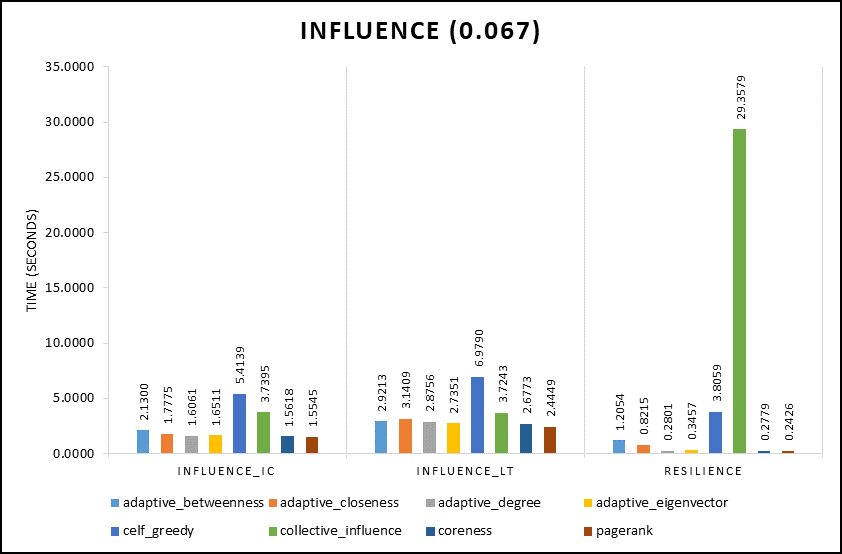
\includegraphics[angle=90, scale=0.65]{automata-influence-4}\par 
				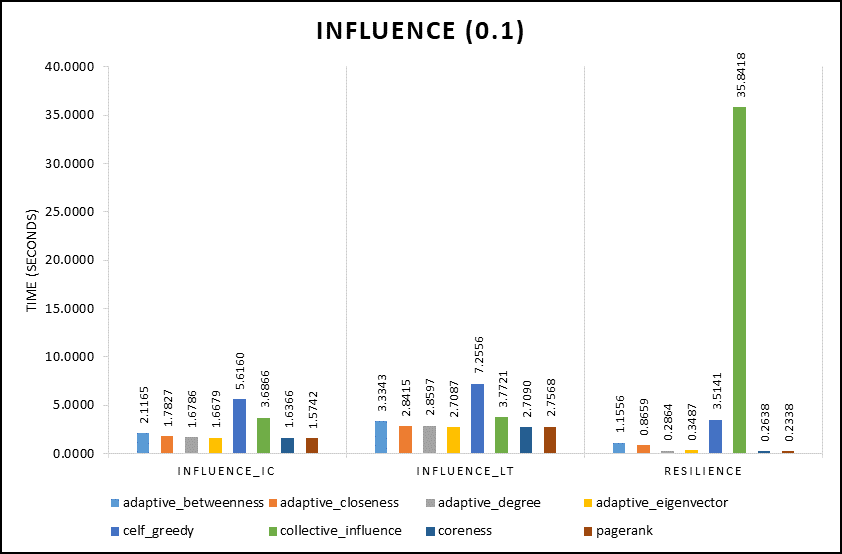
\includegraphics[angle=90, scale=0.65]{automata-influence-5}\par 
			\end{multicols}
			
			\caption{Normalized elapsed time for influence criteria on Automata network.}
			\label{fig:inf-framework-automata3}
		\end{figure*}
		
		
		% *** caida ***
		\begin{figure*}[ht]
			\begin{multicols}{2}
				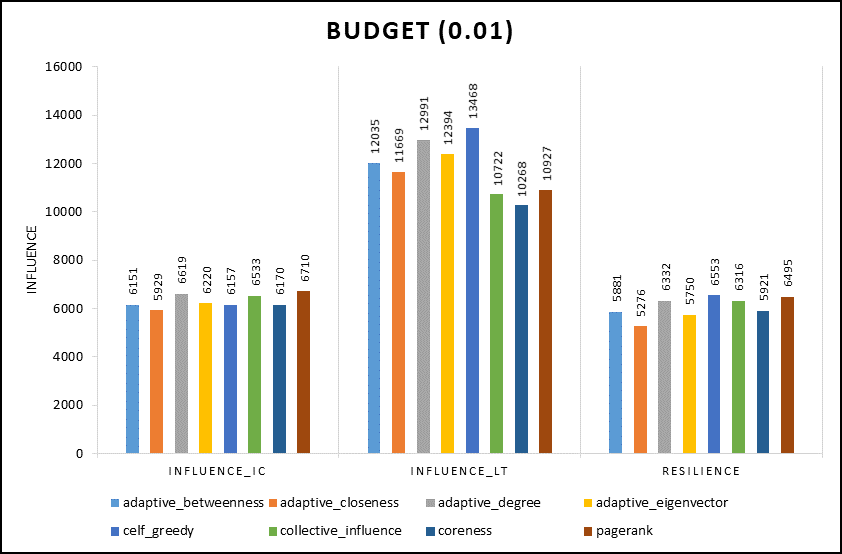
\includegraphics[angle=90, scale=0.65]{caida-budget-1}\par 
				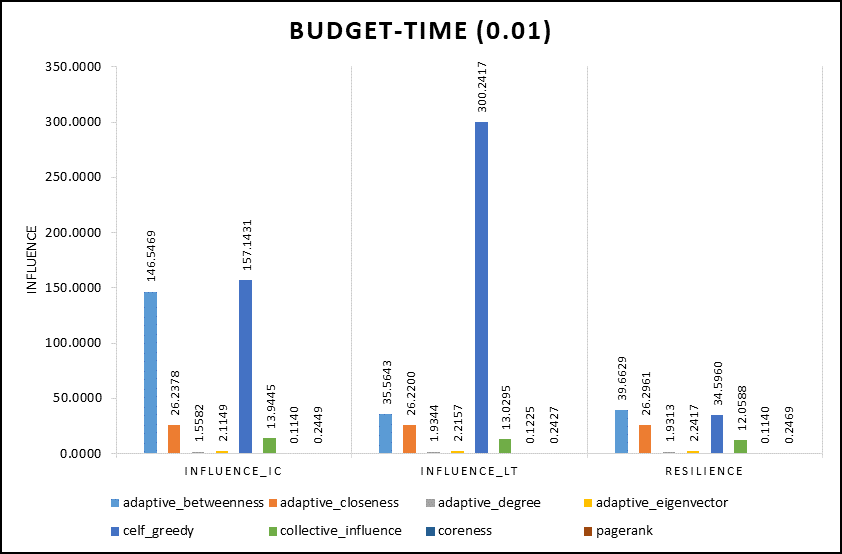
\includegraphics[angle=90, scale=0.65]{caida-budget-time-1}\par 
			\end{multicols}
			\begin{multicols}{2}
				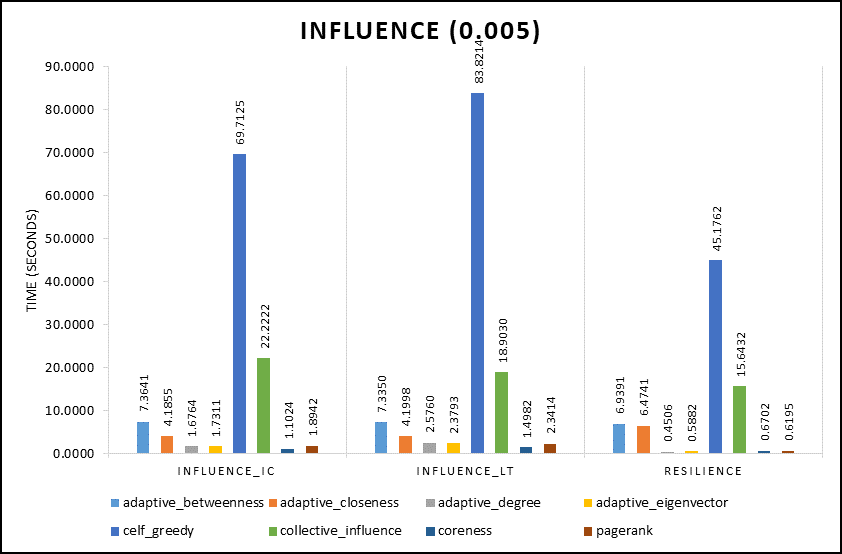
\includegraphics[angle=90, scale=0.65]{caida-influence-1}\par 
			\end{multicols}
			
			\caption{Influence measure (top-left), normalized elapsed time for budget criteria (top-right), and normalized elapsed time for influence criteria (bottom-left) of AS-CAIDA network.}
			\label{fig:inf-framework-caida}
		\end{figure*}
	
		
		% *** city2010 ***
		\begin{figure*}[ht]
			\begin{multicols}{2}
				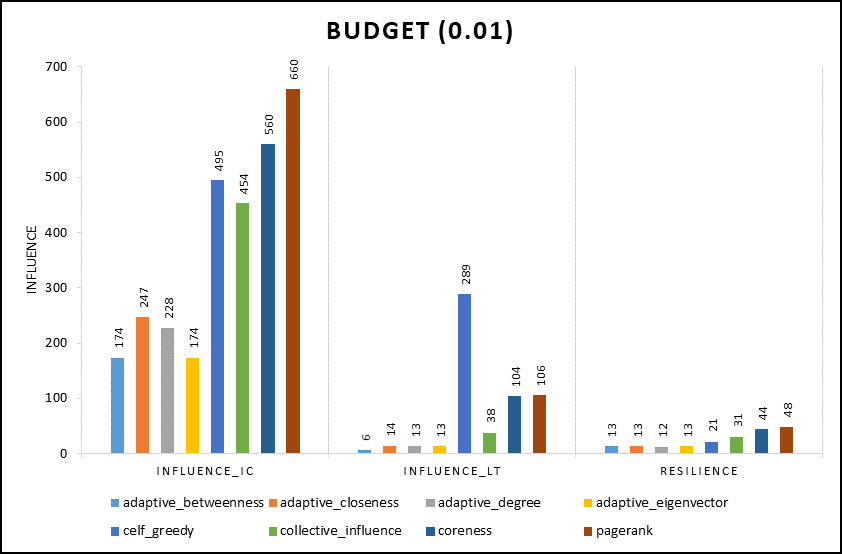
\includegraphics[angle=90, scale=0.65]{city2010-budget-1}\par 
				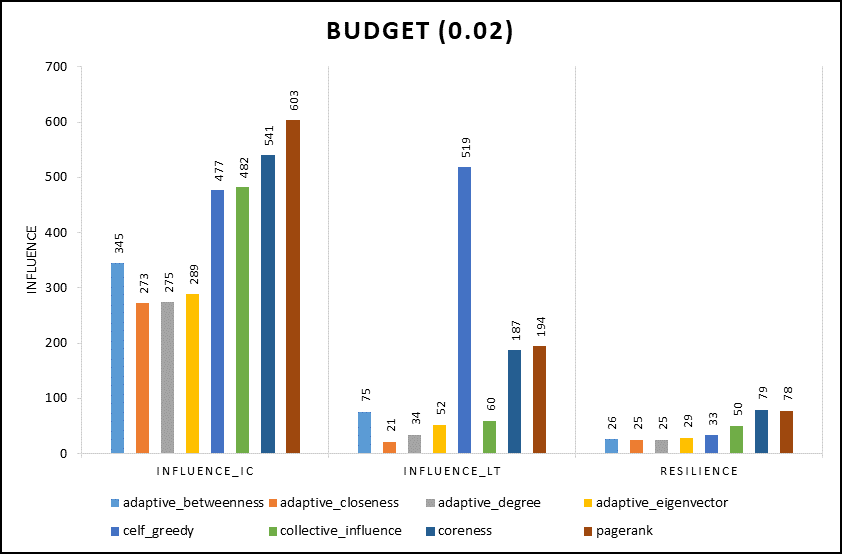
\includegraphics[angle=90, scale=0.65]{city2010-budget-2}\par 
			\end{multicols}
			\begin{multicols}{2}
				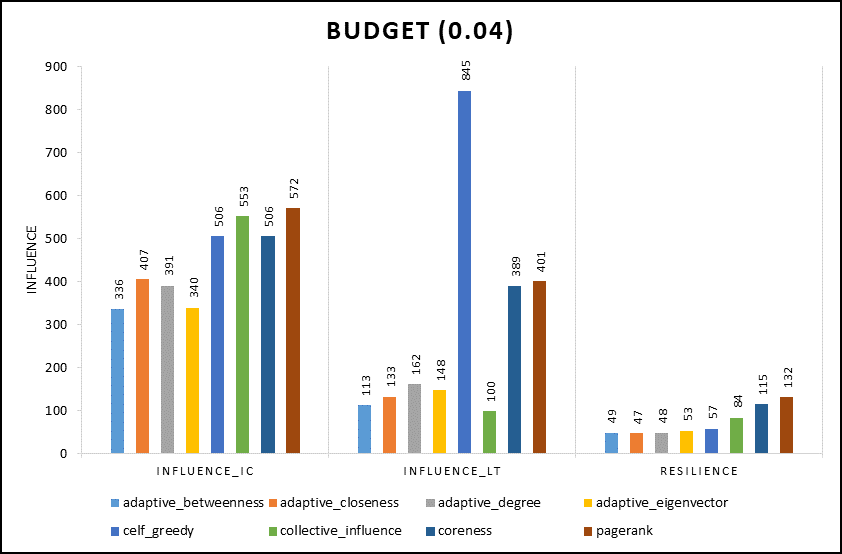
\includegraphics[angle=90, scale=0.65]{city2010-budget-4}\par 
				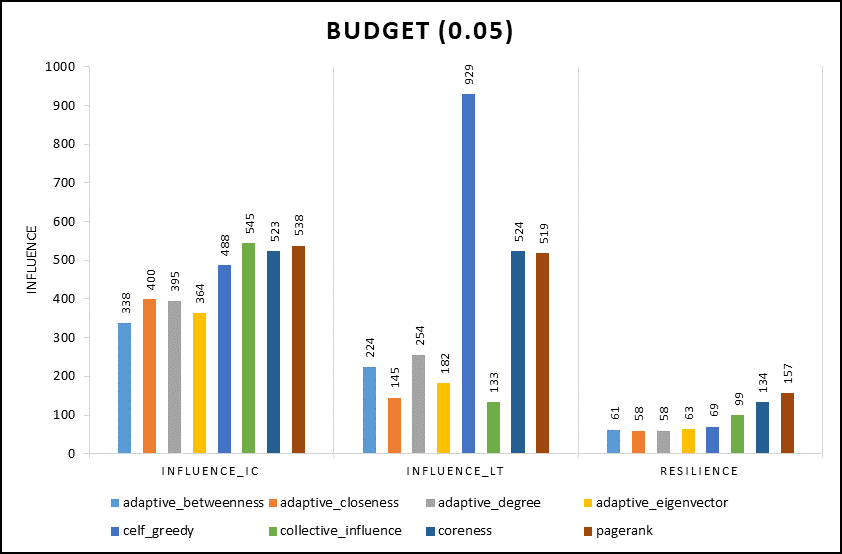
\includegraphics[angle=90, scale=0.65]{city2010-budget-5}\par 
			\end{multicols}
			
			\caption{Influence measure of City network - 2010 on range on all budgets evaluated for all three tests.}
			\label{fig:inf-framework-city2010}
		\end{figure*}
		
		\begin{figure*}[ht]
			\begin{multicols}{2}
				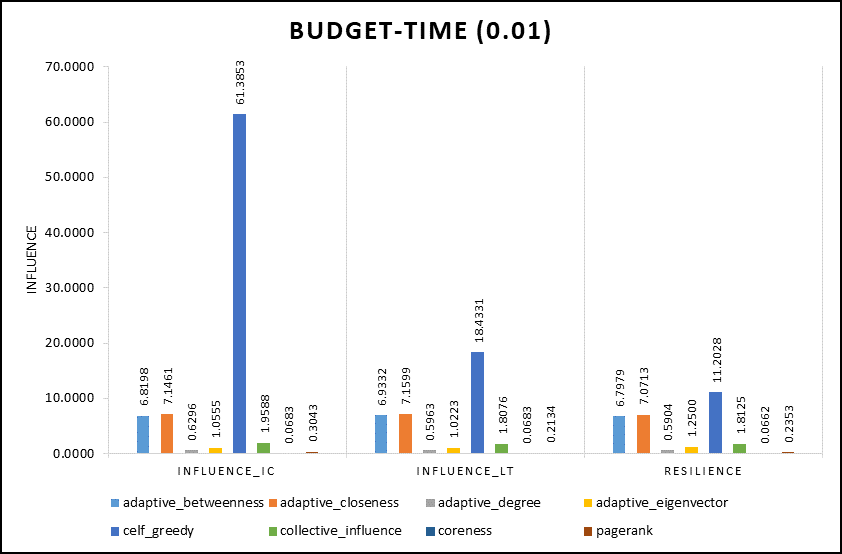
\includegraphics[angle=90, scale=0.65]{city2010-budget-time-1}\par 
				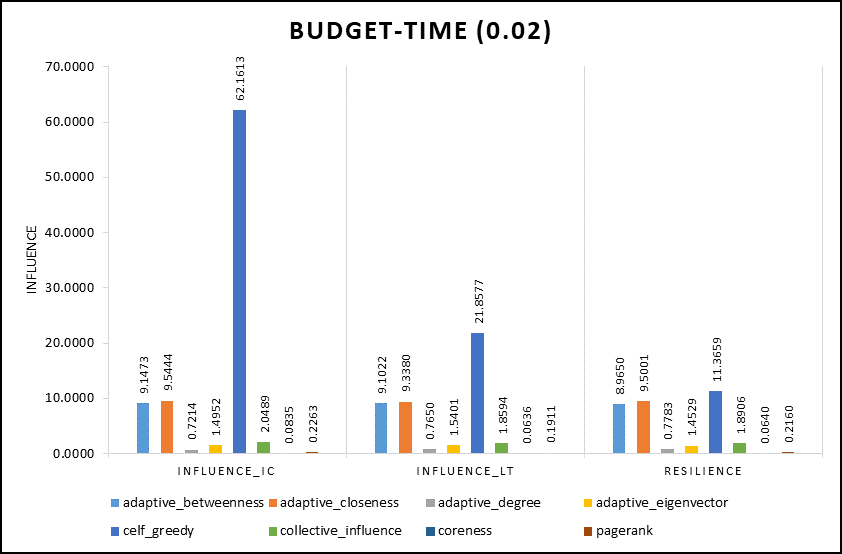
\includegraphics[angle=90, scale=0.65]{city2010-budget-time-2}\par 
			\end{multicols}
			\begin{multicols}{2}
				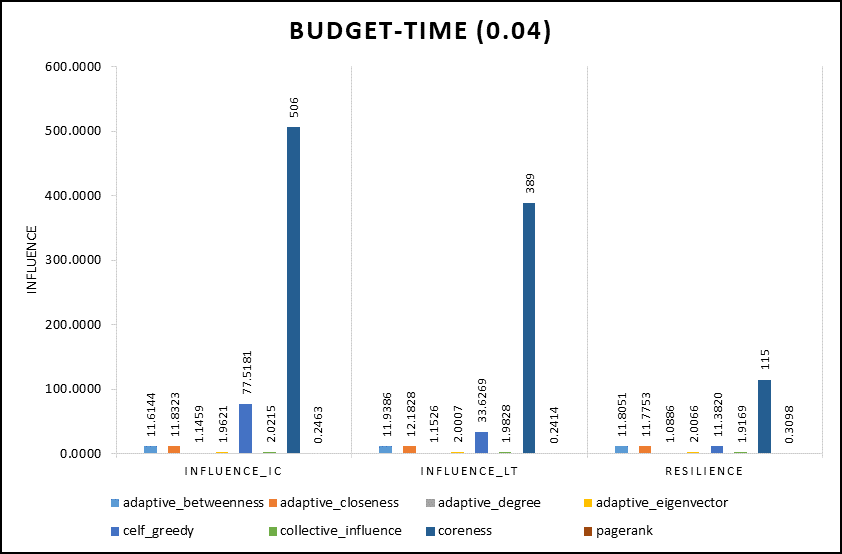
\includegraphics[angle=90, scale=0.65]{city2010-budget-time-4}\par 
				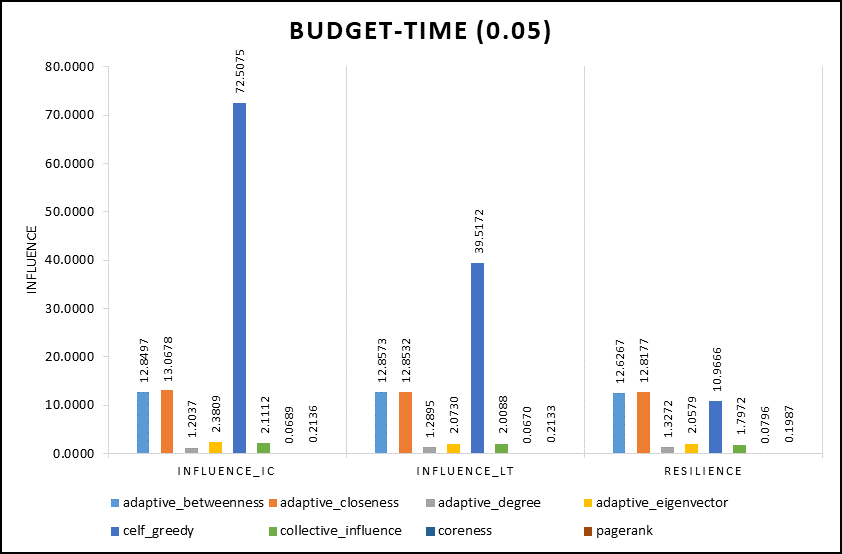
\includegraphics[angle=90, scale=0.65]{city2010-budget-time-5}\par 
			\end{multicols}
			
			\caption{Normalized elapsed time for budget criteria on city2010 network.}
			\label{fig:inf-framework-city2010-2}
		\end{figure*}
		
		\begin{figure*}[h]
			\begin{multicols}{2}
				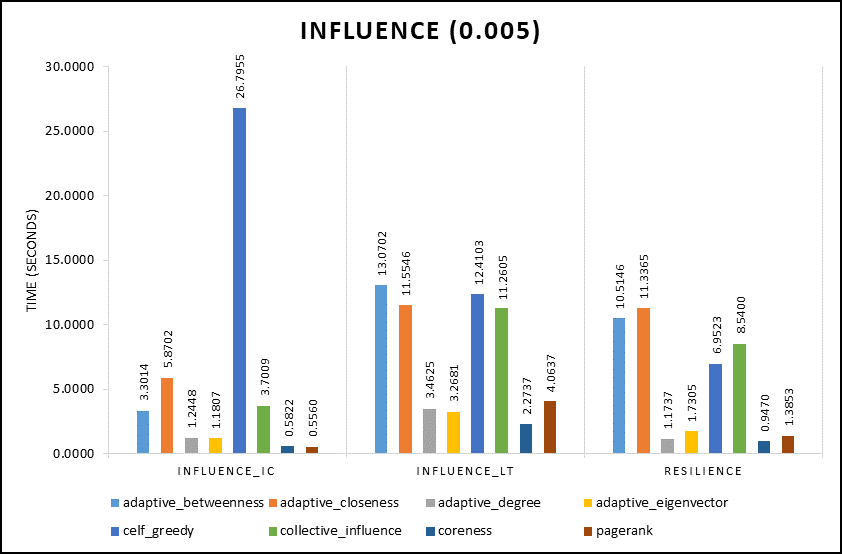
\includegraphics[angle=90, scale=0.65]{city2010-influence-1}\par 
				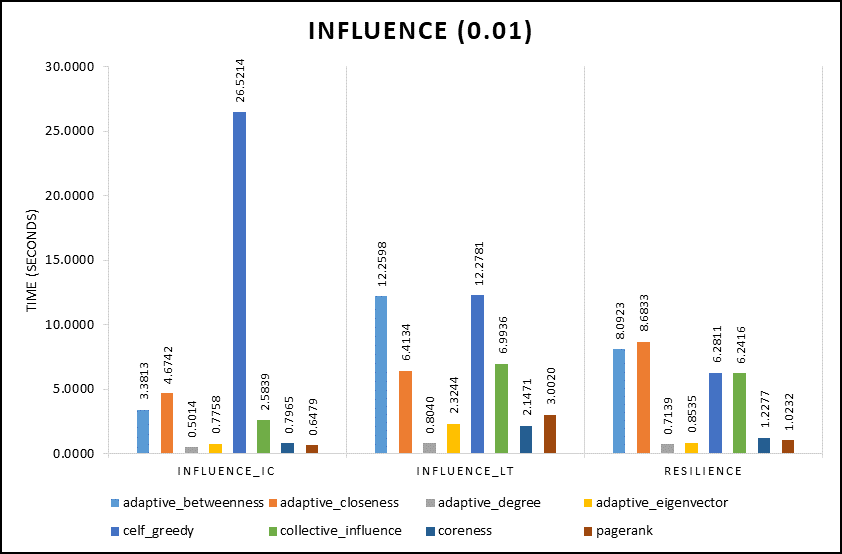
\includegraphics[angle=90, scale=0.65]{city2010-influence-2}\par 
			\end{multicols}
			\begin{multicols}{2}
				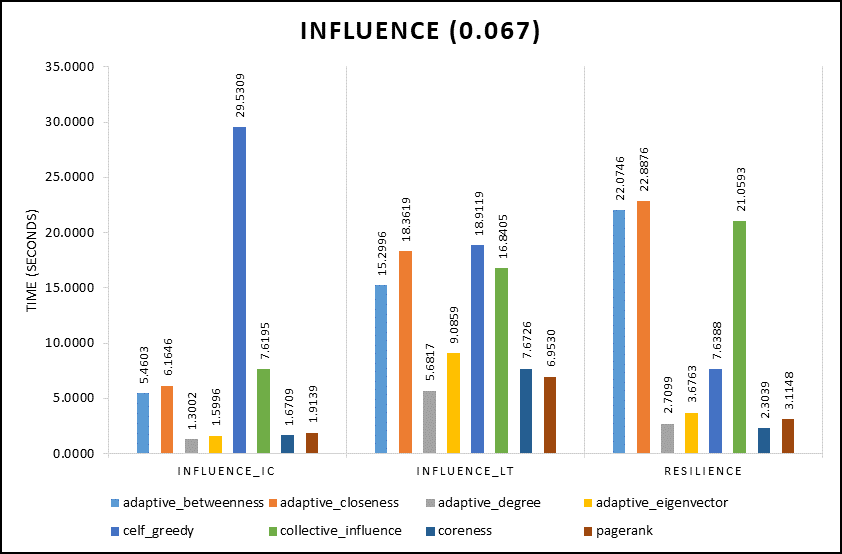
\includegraphics[angle=90, scale=0.65]{city2010-influence-4}\par 
				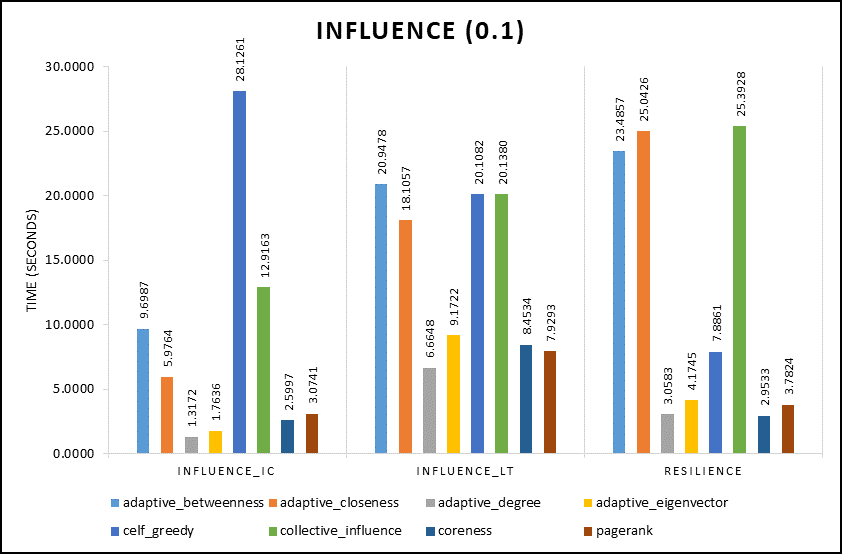
\includegraphics[angle=90, scale=0.65]{city2010-influence-5}\par 
			\end{multicols}
			
			\caption{Normalized elapsed time for influence criteria on City network - 2010.}
			\label{fig:inf-framework-city2010-3}
		\end{figure*}
		
		
		% *** city2013 ***
		\begin{figure*}[ht]
			\begin{multicols}{2}
				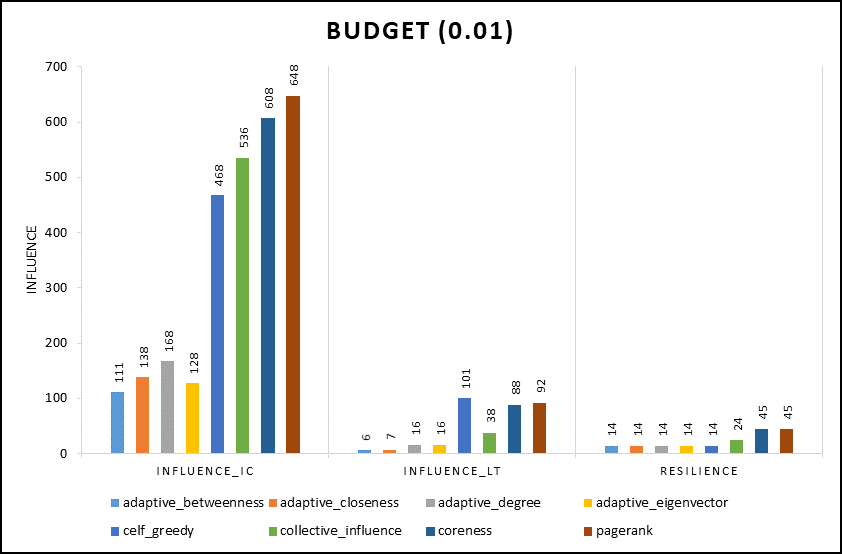
\includegraphics[angle=90, scale=0.65]{city2013-budget-1}\par 
				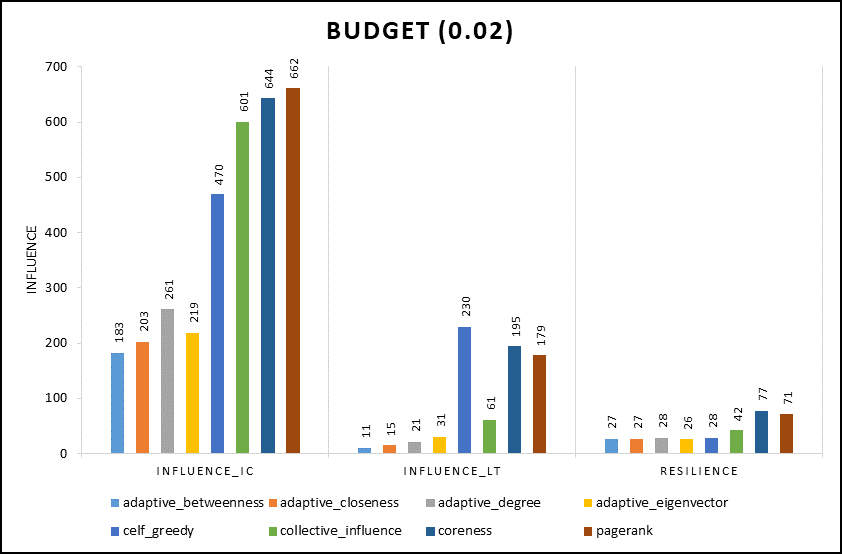
\includegraphics[angle=90, scale=0.65]{city2013-budget-2}\par 
			\end{multicols}
			\begin{multicols}{2}
				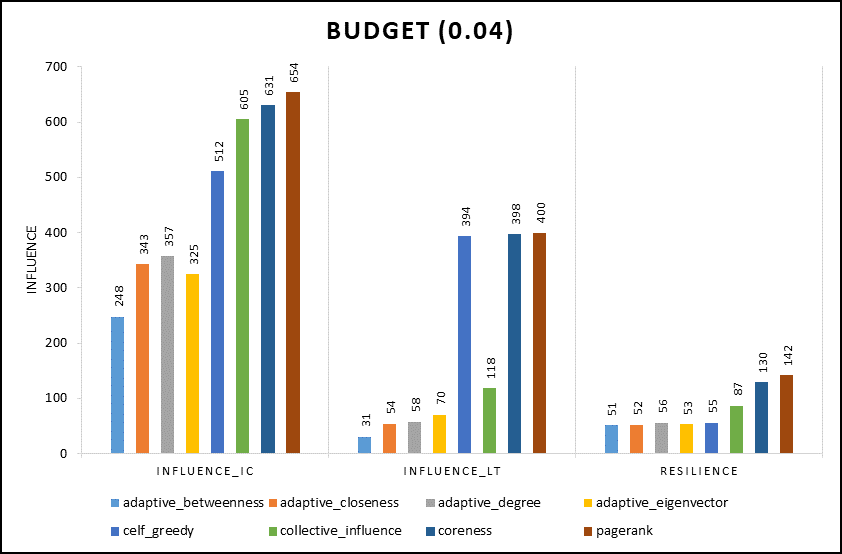
\includegraphics[angle=90, scale=0.65]{city2013-budget-4}\par 
				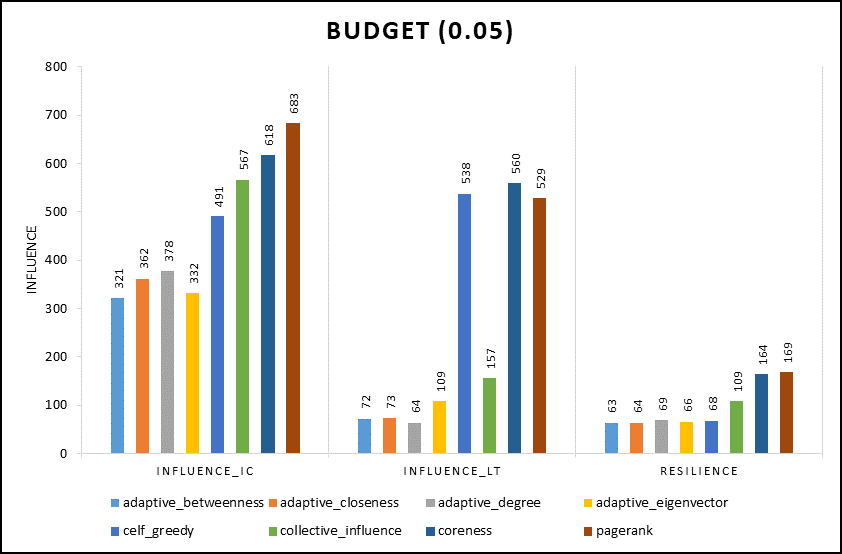
\includegraphics[angle=90, scale=0.65]{city2013-budget-5}\par 
			\end{multicols}
			
			\caption{Influence measure of City network - 2013 on range on all budgets evaluated for all three tests.}
			\label{fig:inf-framework-city2013}
		\end{figure*}
		
		\begin{figure*}[ht]
			\begin{multicols}{2}
				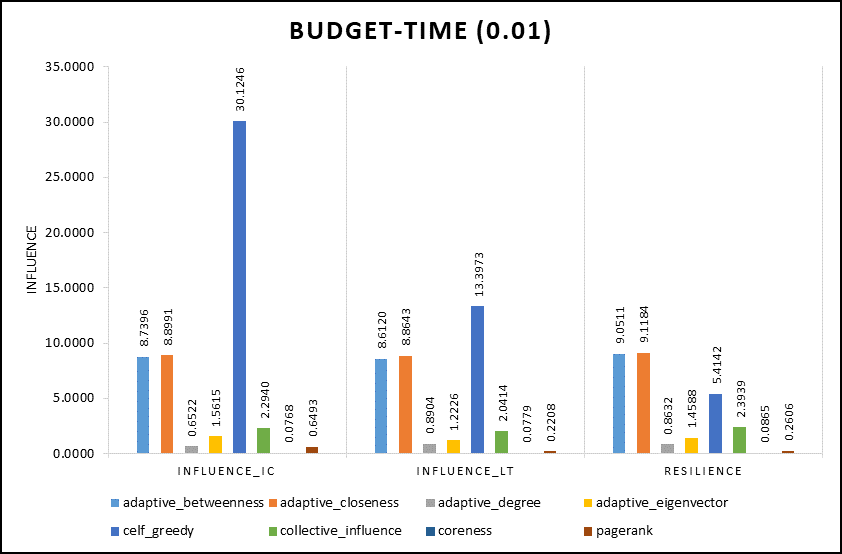
\includegraphics[angle=90, scale=0.65]{city2013-budget-time-1}\par 
				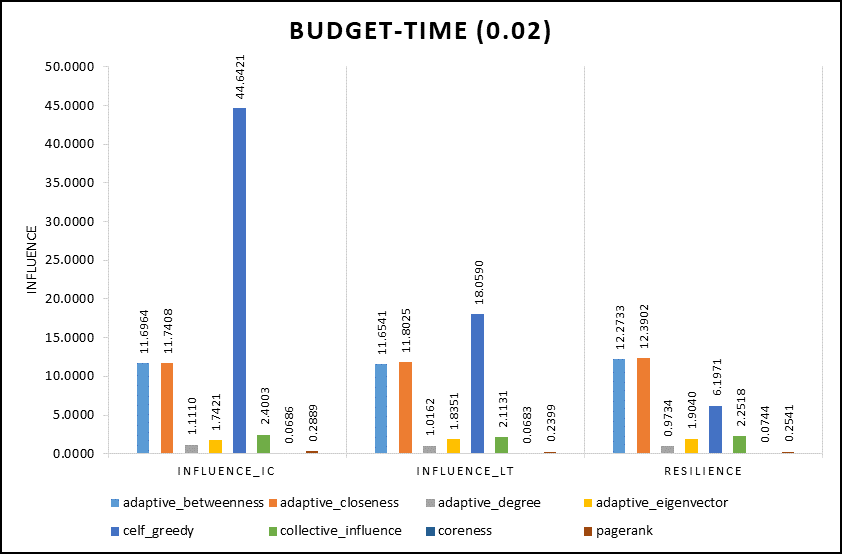
\includegraphics[angle=90, scale=0.65]{city2013-budget-time-2}\par 
			\end{multicols}
			\begin{multicols}{2}
				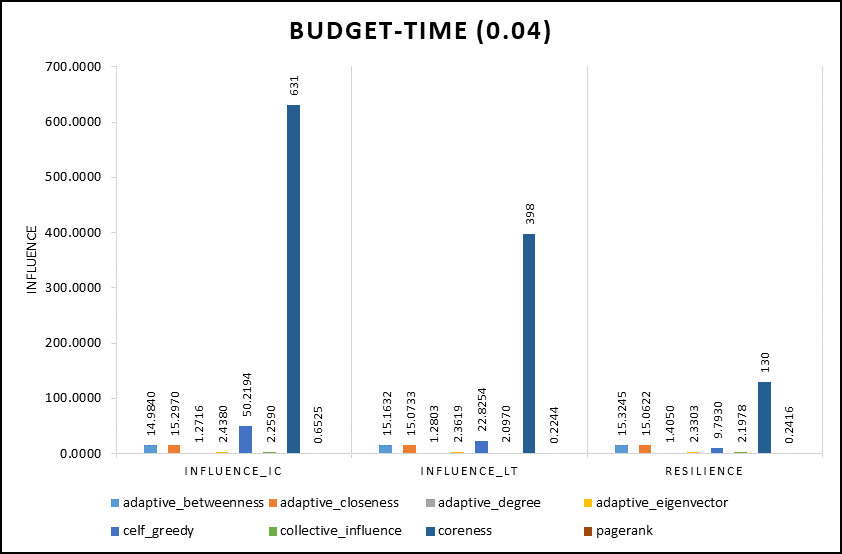
\includegraphics[angle=90, scale=0.65]{city2013-budget-time-4}\par 
				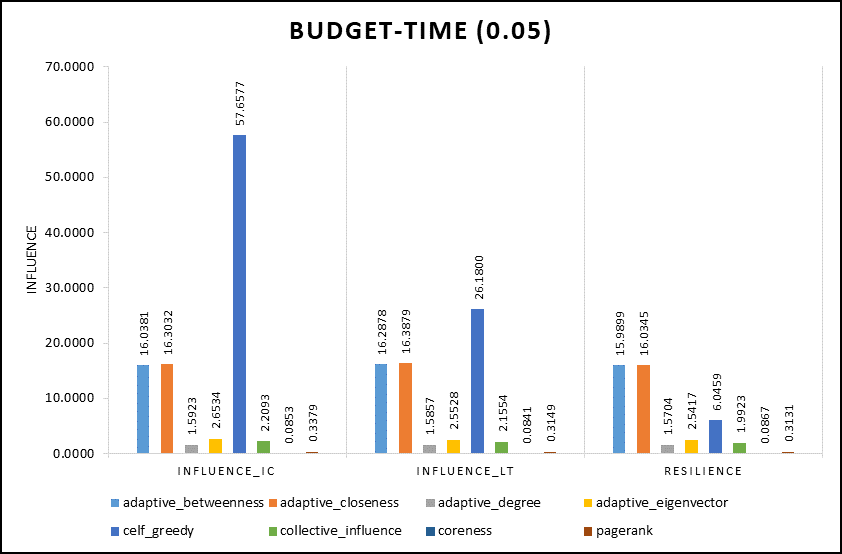
\includegraphics[angle=90, scale=0.65]{city2013-budget-time-5}\par 
			\end{multicols}
			
			\caption{Normalized elapsed time for budget criteria on city2013 network.}
			\label{fig:inf-framework-city2013-2}
		\end{figure*}
		
		\begin{figure*}[h]
			\begin{multicols}{2}
				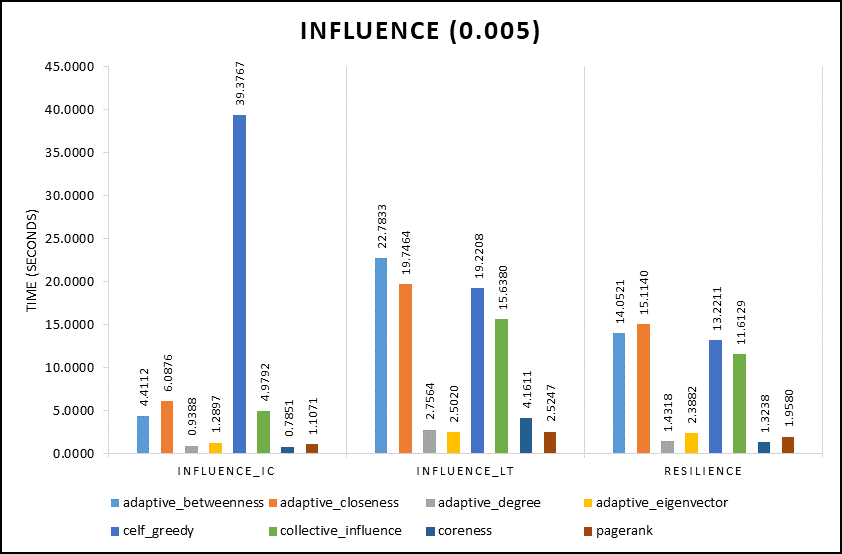
\includegraphics[angle=90, scale=0.65]{city2013-influence-1}\par 
				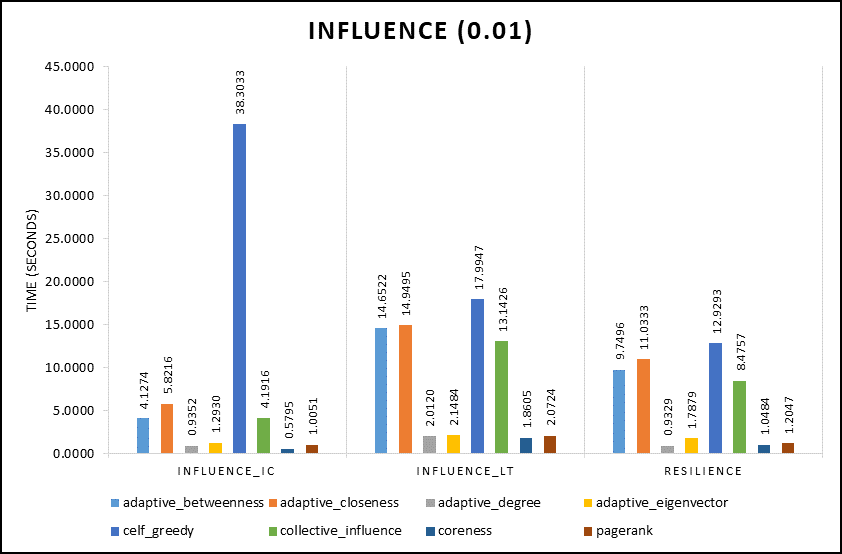
\includegraphics[angle=90, scale=0.65]{city2013-influence-2}\par 
			\end{multicols}
			\begin{multicols}{2}
				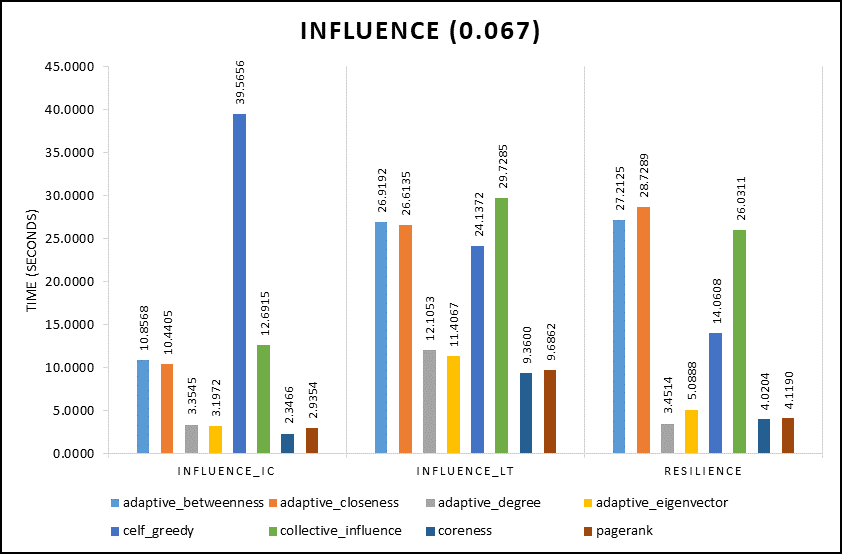
\includegraphics[angle=90, scale=0.65]{city2013-influence-4}\par 
				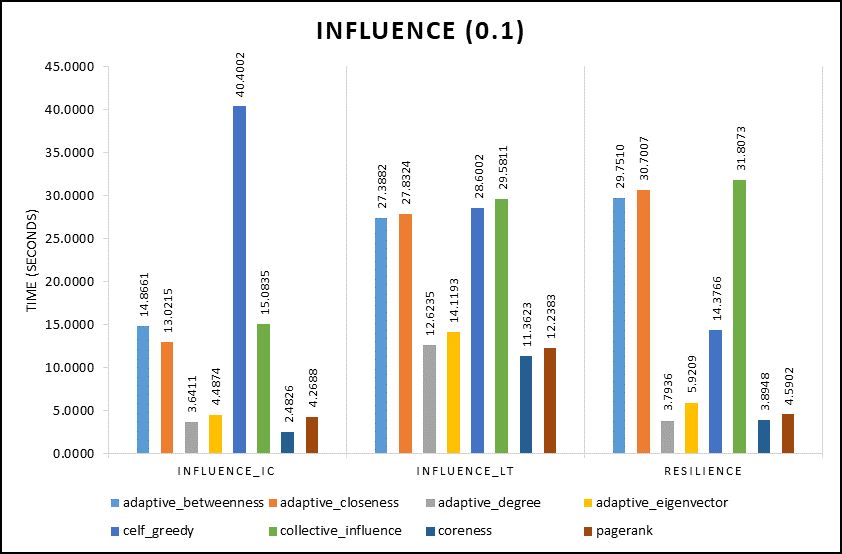
\includegraphics[angle=90, scale=0.65]{city2013-influence-5}\par 
			\end{multicols}
			
			\caption{Normalized elapsed time for influence criteria on City network - 2013.}
			\label{fig:inf-framework-city2013-3}
		\end{figure*}
		
		
		% *** city2016 ***
		\begin{figure*}[ht]
			\begin{multicols}{2}
				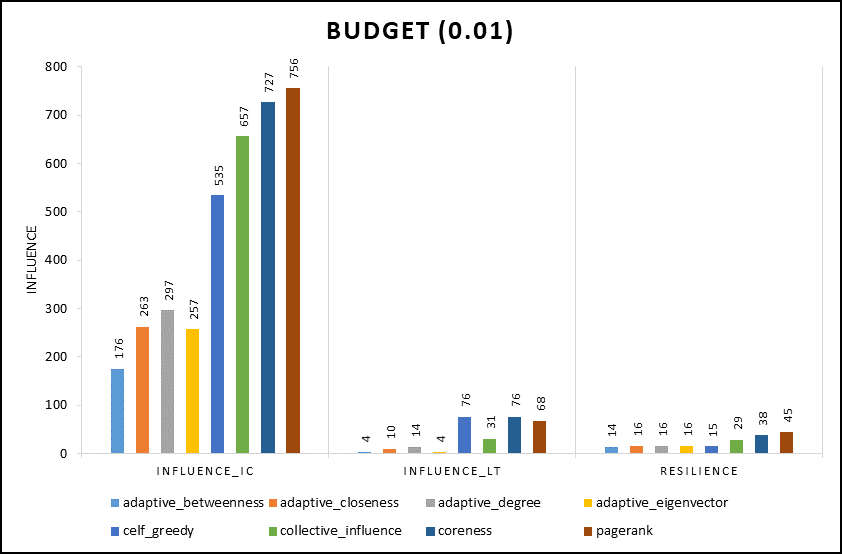
\includegraphics[angle=90, scale=0.65]{city2016-budget-1}\par 
				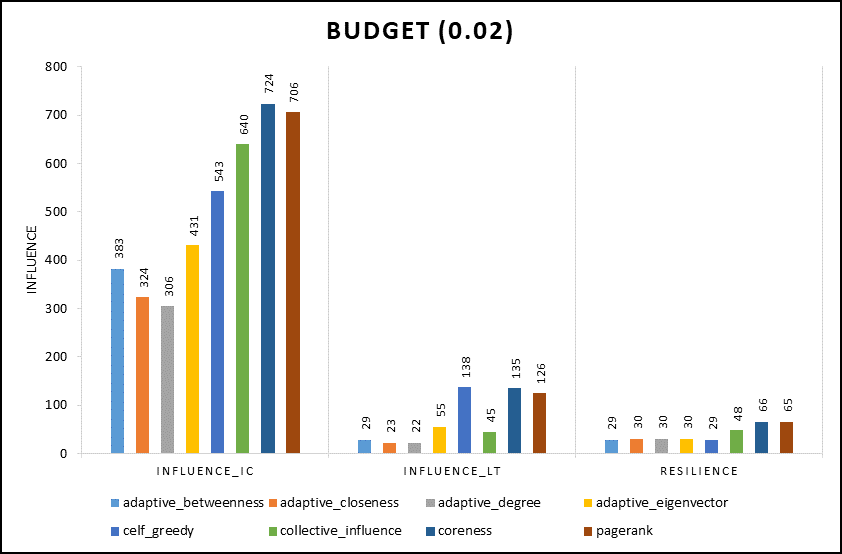
\includegraphics[angle=90, scale=0.65]{city2016-budget-2}\par 
			\end{multicols}
			\begin{multicols}{2}
				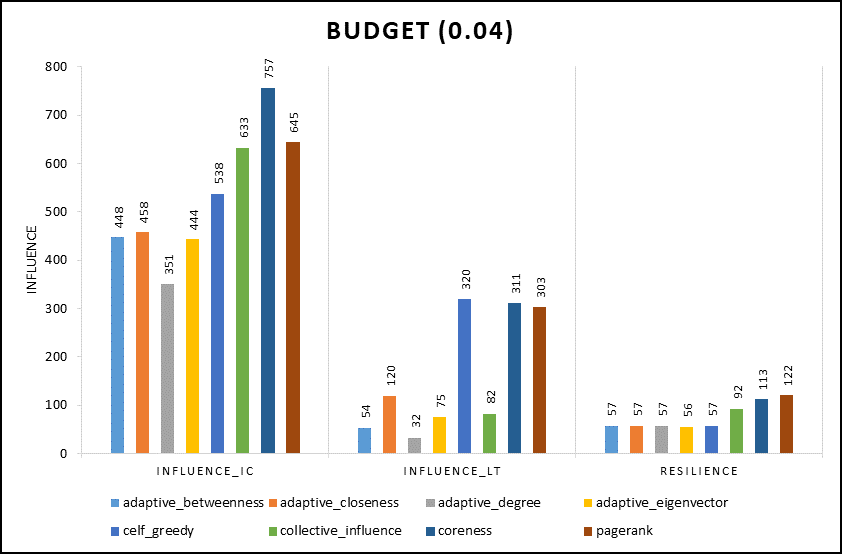
\includegraphics[angle=90, scale=0.65]{city2016-budget-4}\par 
				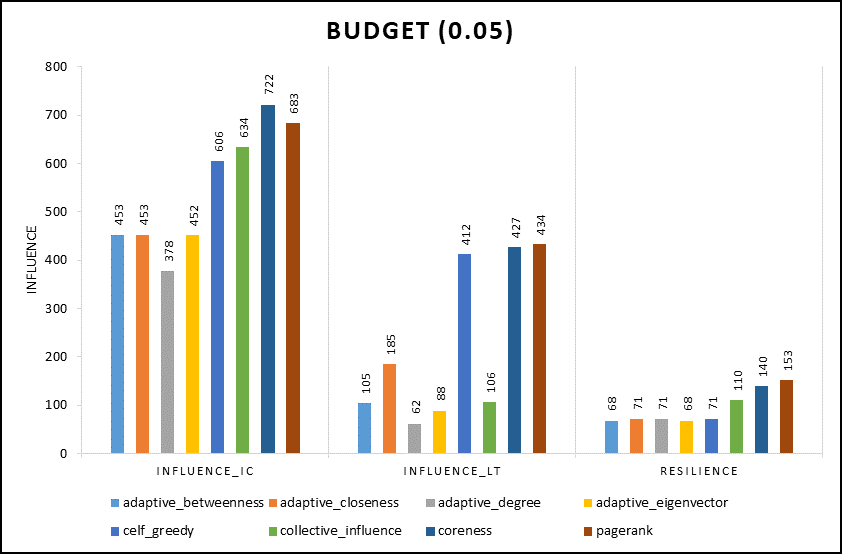
\includegraphics[angle=90, scale=0.65]{city2016-budget-5}\par 
			\end{multicols}
			
			\caption{Influence measure of City network - 2016 on range on all budgets evaluated for all three tests.}
			\label{fig:inf-framework-city2016}
		\end{figure*}
		
		\begin{figure*}[ht]
			\begin{multicols}{2}
				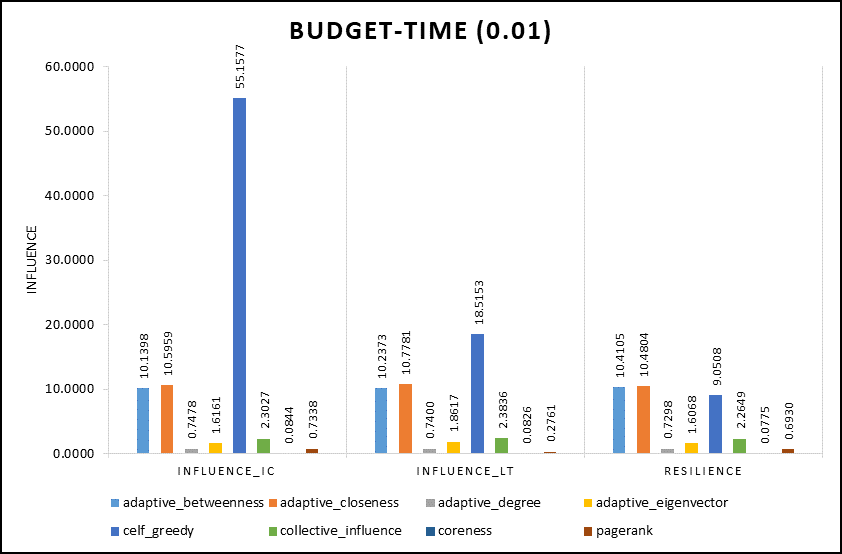
\includegraphics[angle=90, scale=0.65]{city2016-budget-time-1}\par 
				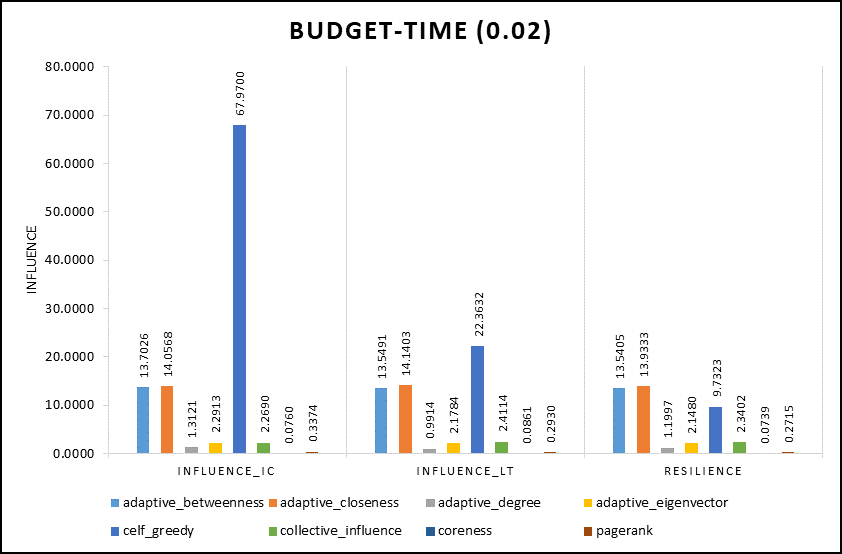
\includegraphics[angle=90, scale=0.65]{city2016-budget-time-2}\par 
			\end{multicols}
			\begin{multicols}{2}
				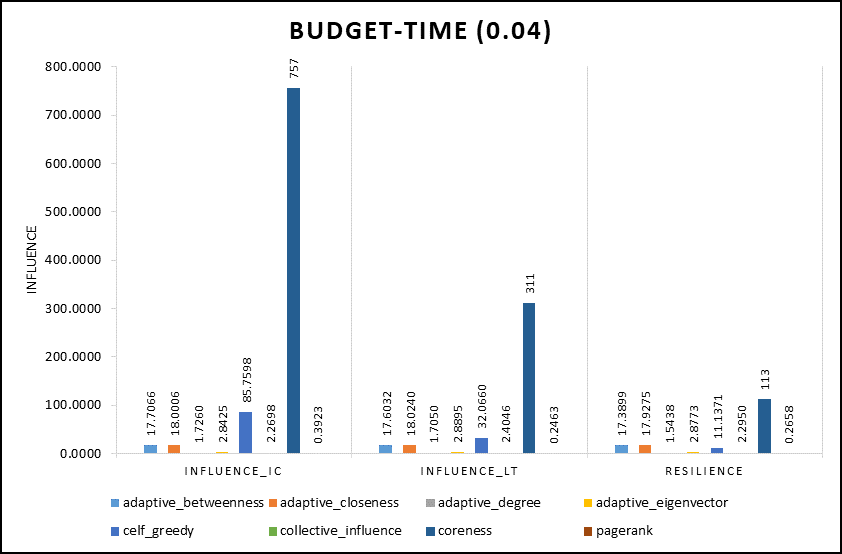
\includegraphics[angle=90, scale=0.65]{city2016-budget-time-4}\par 
				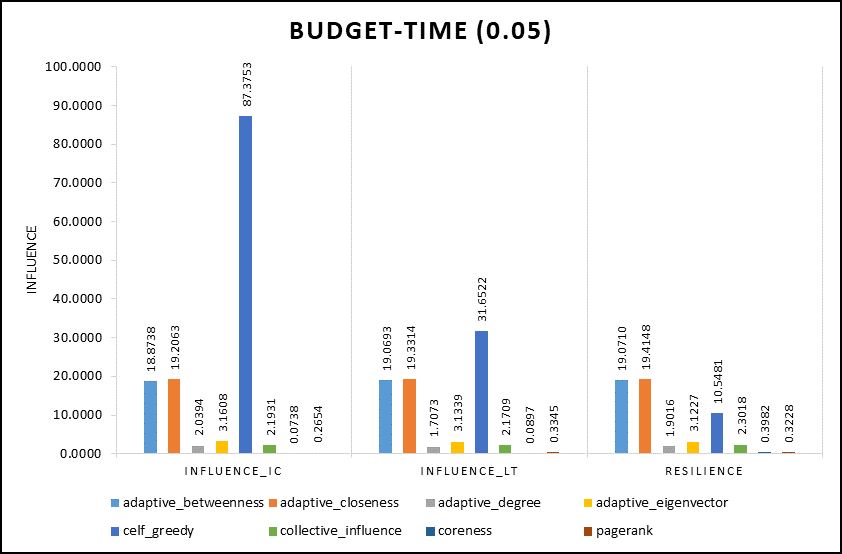
\includegraphics[angle=90, scale=0.65]{city2016-budget-time-5}\par 
			\end{multicols}
			
			\caption{Normalized elapsed time for budget criteria on city2016 network.}
			\label{fig:inf-framework-city2016-2}
		\end{figure*}
		
		\begin{figure*}[h]
			\begin{multicols}{2}
				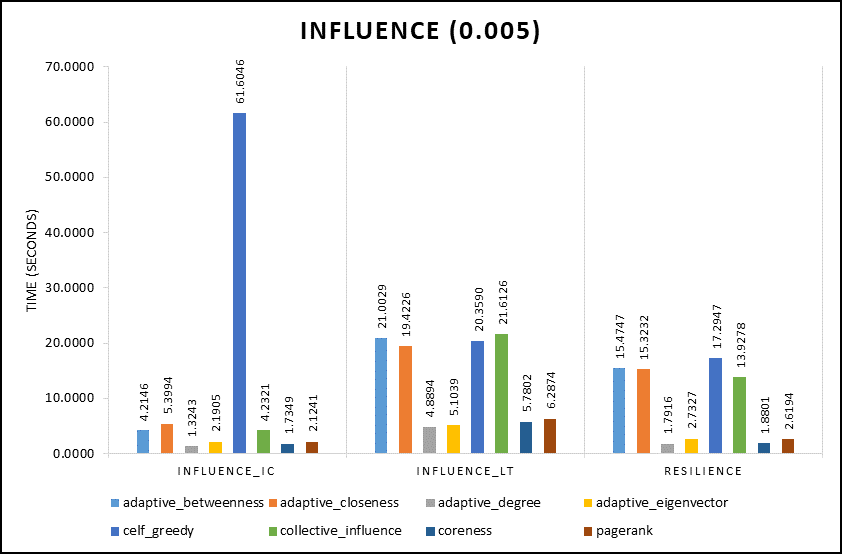
\includegraphics[angle=90, scale=0.65]{city2016-influence-1}\par 
				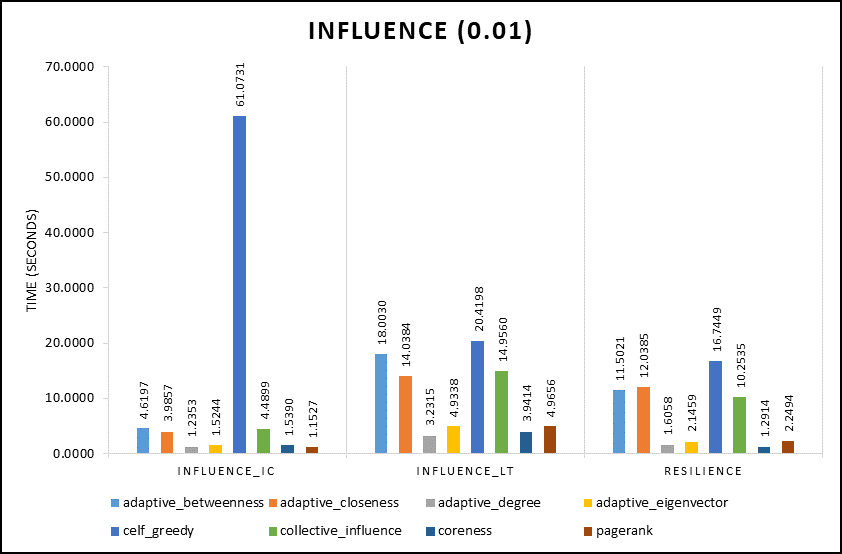
\includegraphics[angle=90, scale=0.65]{city2016-influence-2}\par 
			\end{multicols}
			\begin{multicols}{2}
				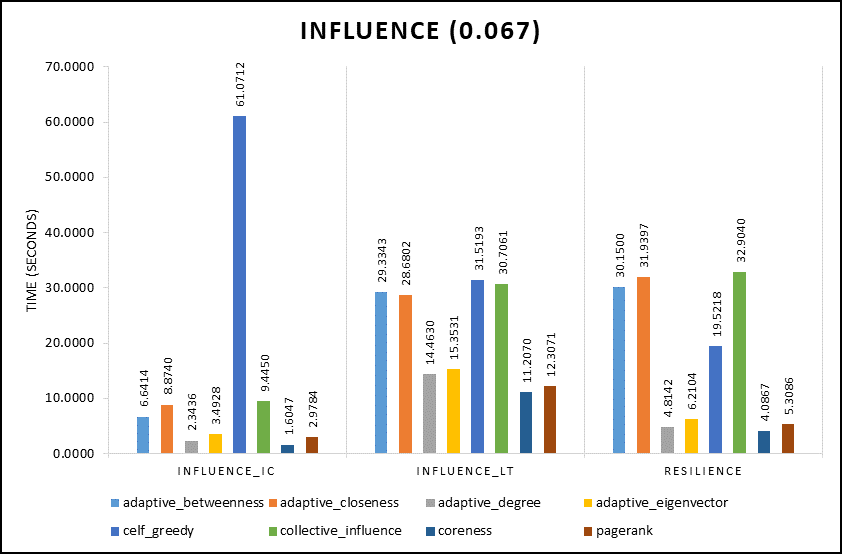
\includegraphics[angle=90, scale=0.65]{city2016-influence-4}\par 
				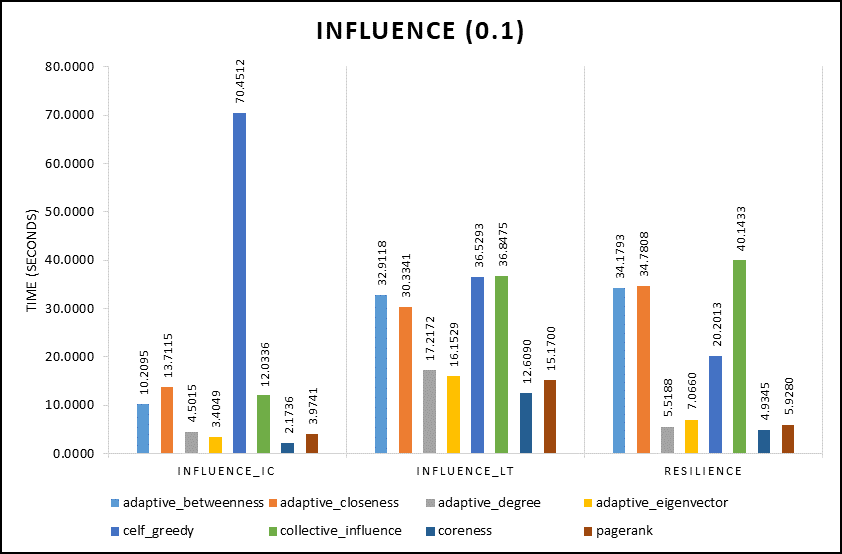
\includegraphics[angle=90, scale=0.65]{city2016-influence-5}\par 
			\end{multicols}
			
			\caption{Normalized elapsed time for influence criteria on City network - 2016.}
			\label{fig:inf-framework-city2016-3}
		\end{figure*}
		
		
		% *** city2019 ***
		\begin{figure*}[ht]
			\begin{multicols}{2}
				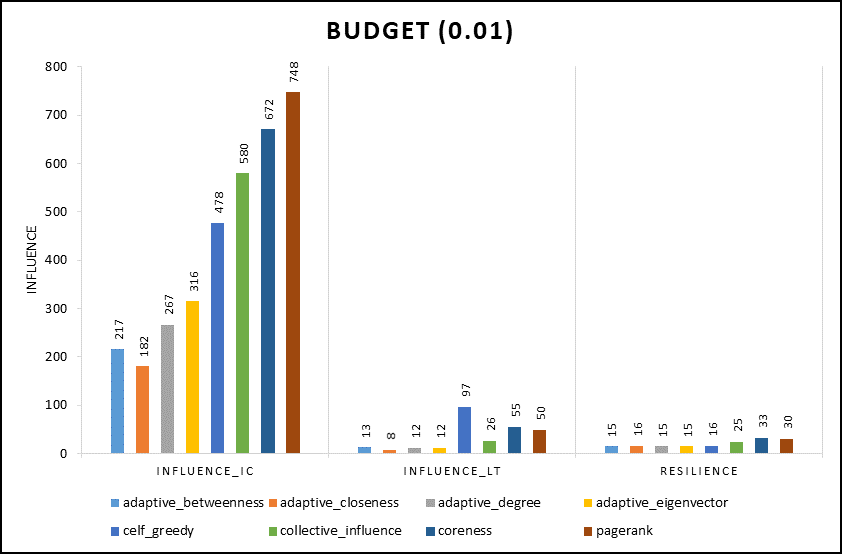
\includegraphics[angle=90, scale=0.65]{city2019-budget-1}\par 
				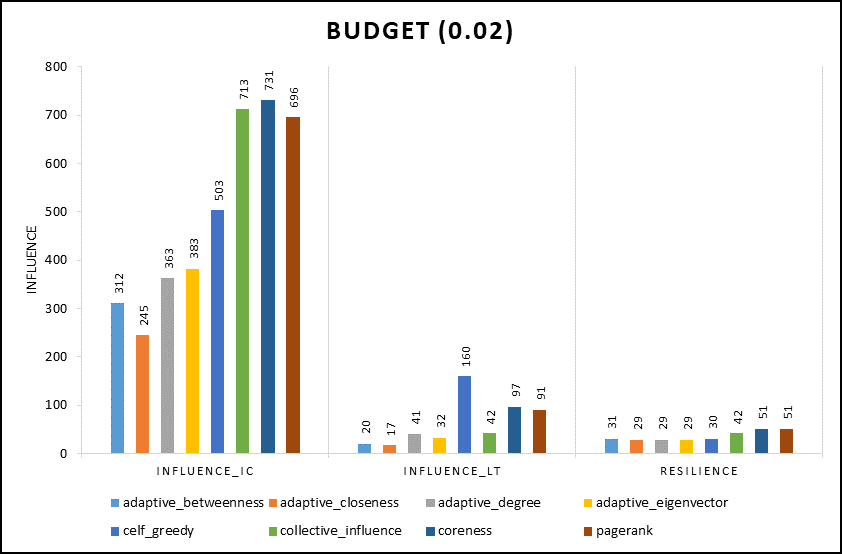
\includegraphics[angle=90, scale=0.65]{city2019-budget-2}\par 
			\end{multicols}
			\begin{multicols}{2}
				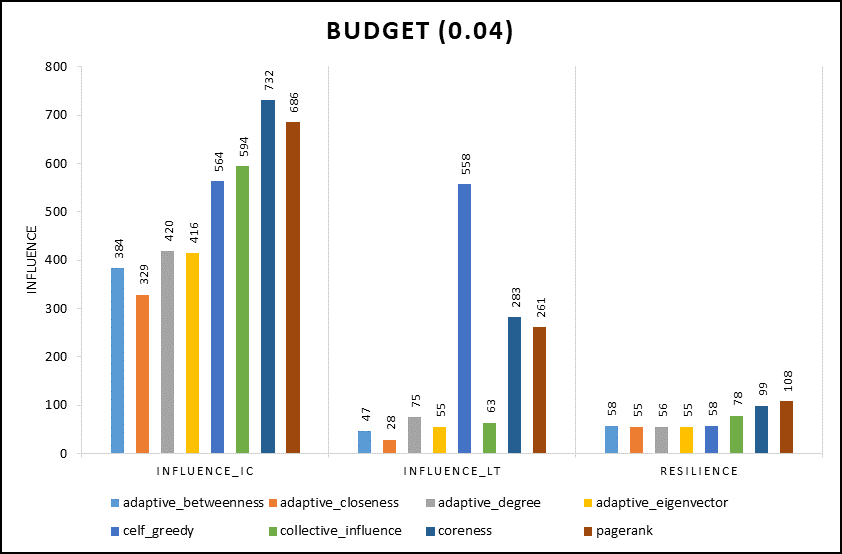
\includegraphics[angle=90, scale=0.65]{city2019-budget-4}\par 
				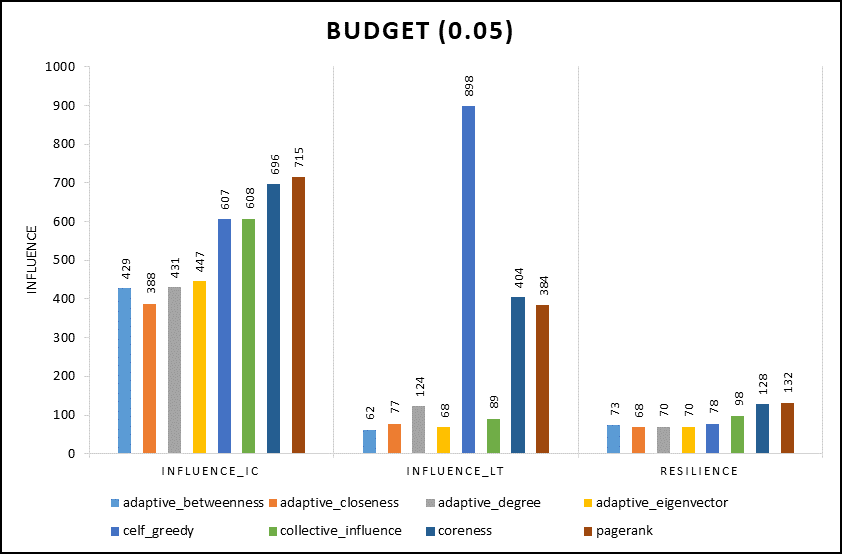
\includegraphics[angle=90, scale=0.65]{city2019-budget-5}\par 
			\end{multicols}
			
			\caption{Influence measure of City network - 2019 on range on all budgets evaluated for all three tests.}
			\label{fig:inf-framework-city2019}
		\end{figure*}
		
		\begin{figure*}[ht]
			\begin{multicols}{2}
				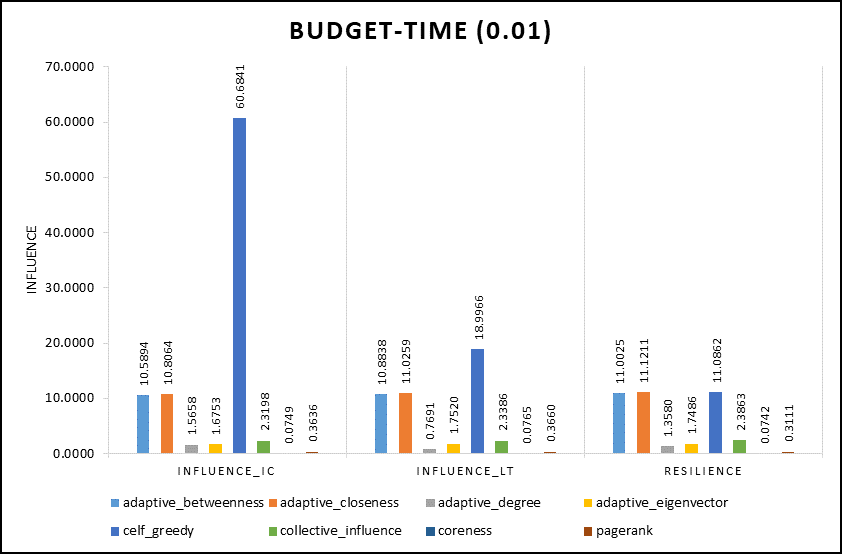
\includegraphics[angle=90, scale=0.65]{city2019-budget-time-1}\par 
				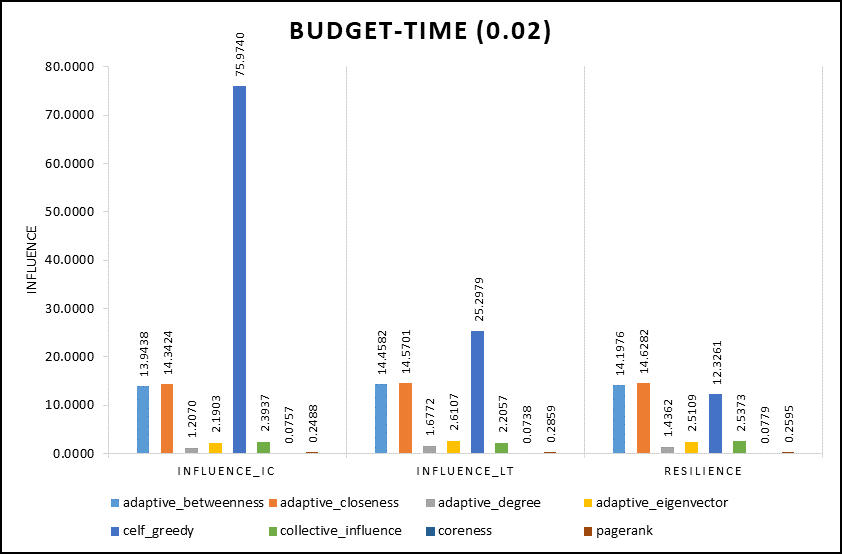
\includegraphics[angle=90, scale=0.65]{city2019-budget-time-2}\par 
			\end{multicols}
			\begin{multicols}{2}
				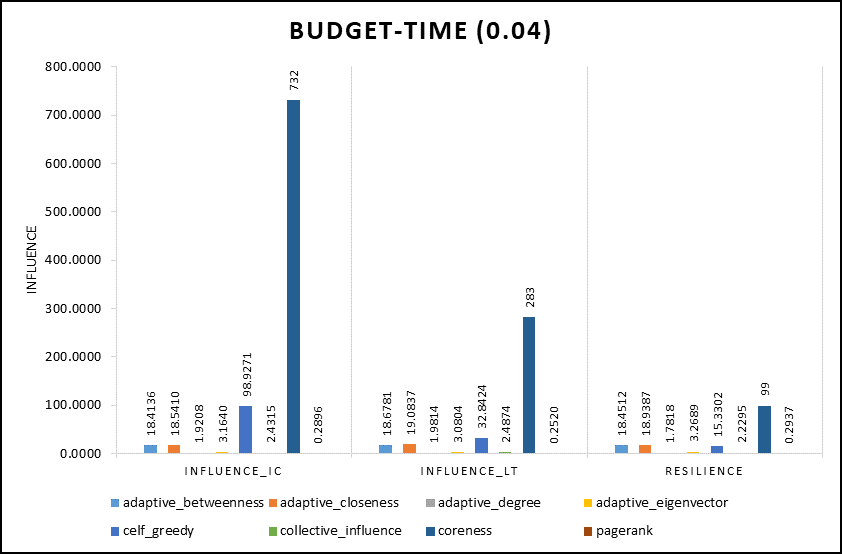
\includegraphics[angle=90, scale=0.65]{city2019-budget-time-4}\par 
				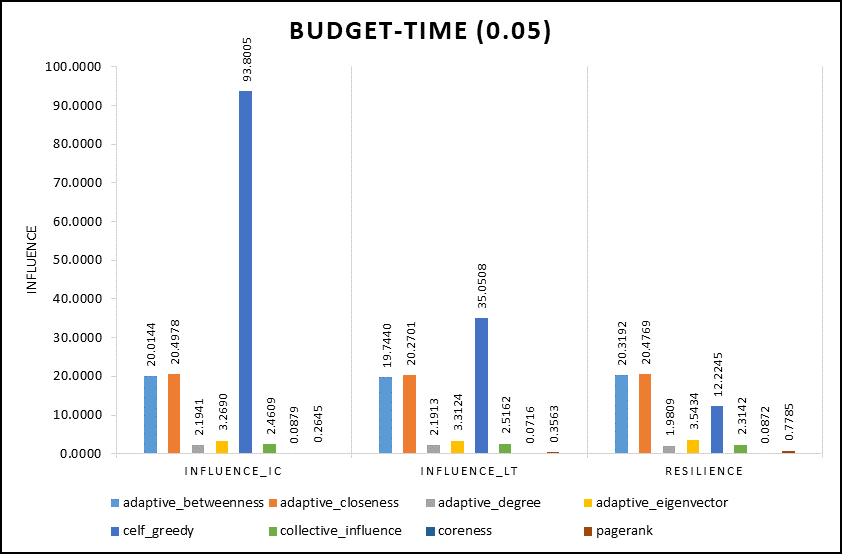
\includegraphics[angle=90, scale=0.65]{city2019-budget-time-5}\par 
			\end{multicols}
			
			\caption{Normalized elapsed time for budget criteria on city2019 network.}
			\label{fig:inf-framework-city2019-2}
		\end{figure*}
		
		\begin{figure*}[h]
			\begin{multicols}{2}
				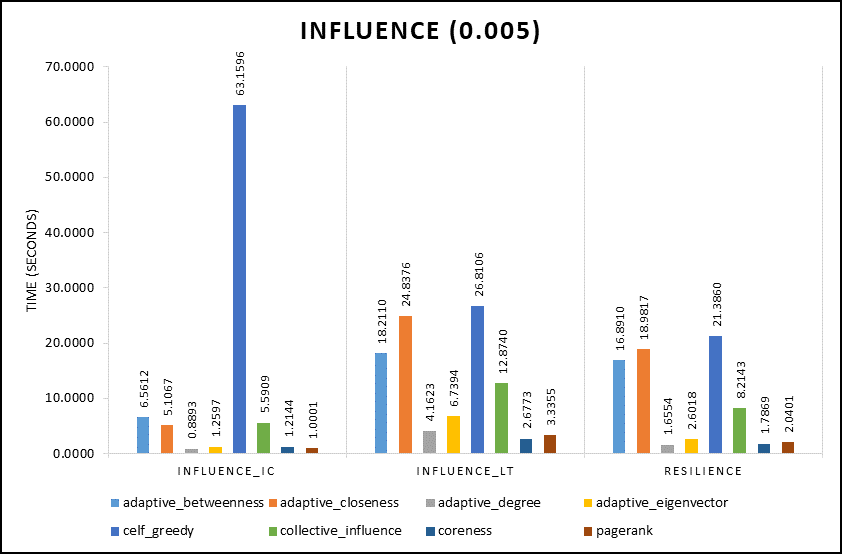
\includegraphics[angle=90, scale=0.65]{city2019-influence-1}\par 
				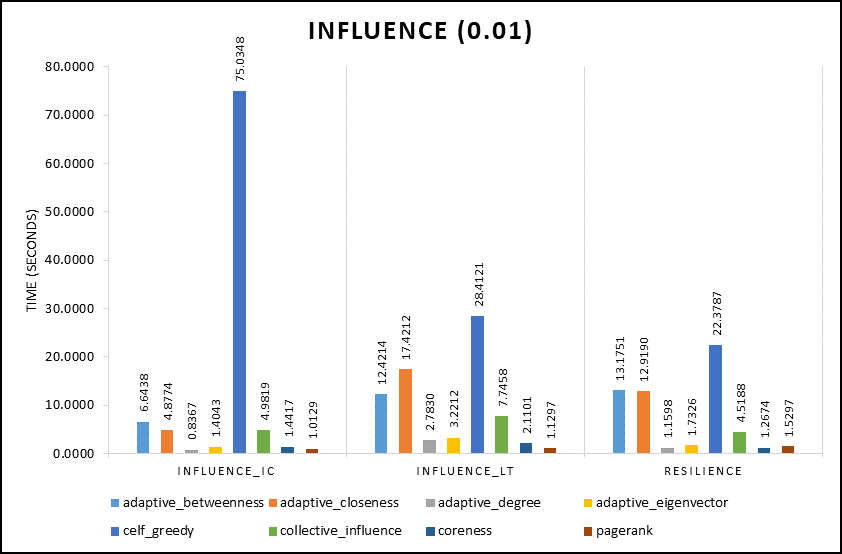
\includegraphics[angle=90, scale=0.65]{city2019-influence-2}\par 
			\end{multicols}
			\begin{multicols}{2}
				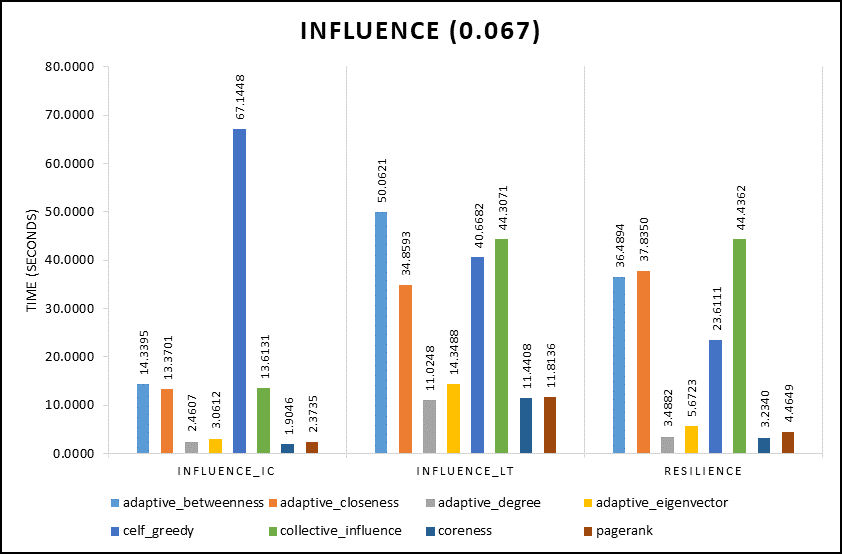
\includegraphics[angle=90, scale=0.65]{city2019-influence-4}\par 
				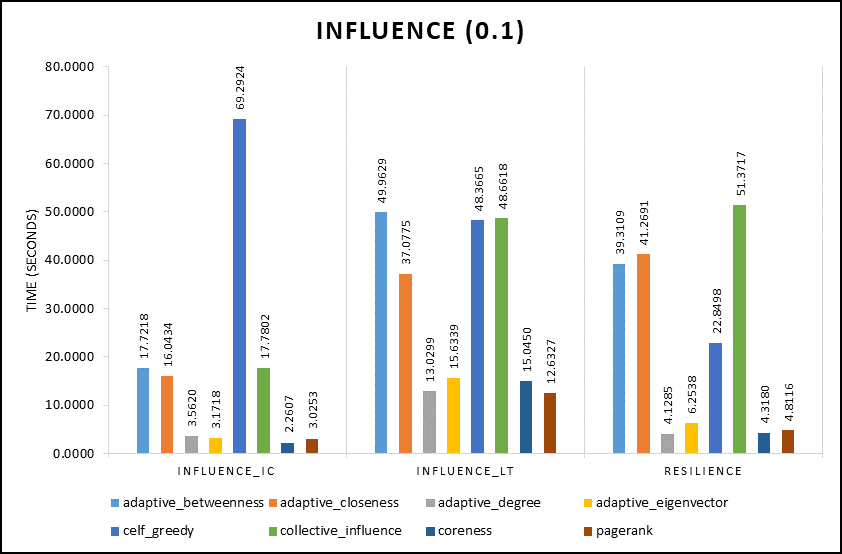
\includegraphics[angle=90, scale=0.65]{city2019-influence-5}\par 
			\end{multicols}
			
			\caption{Normalized elapsed time for influence criteria on City network - 2019.}
			\label{fig:inf-framework-city2019-3}
		\end{figure*}
		
		
		% *** fb_johnshopkins ***
		\begin{figure*}[ht]
			\begin{multicols}{2}
				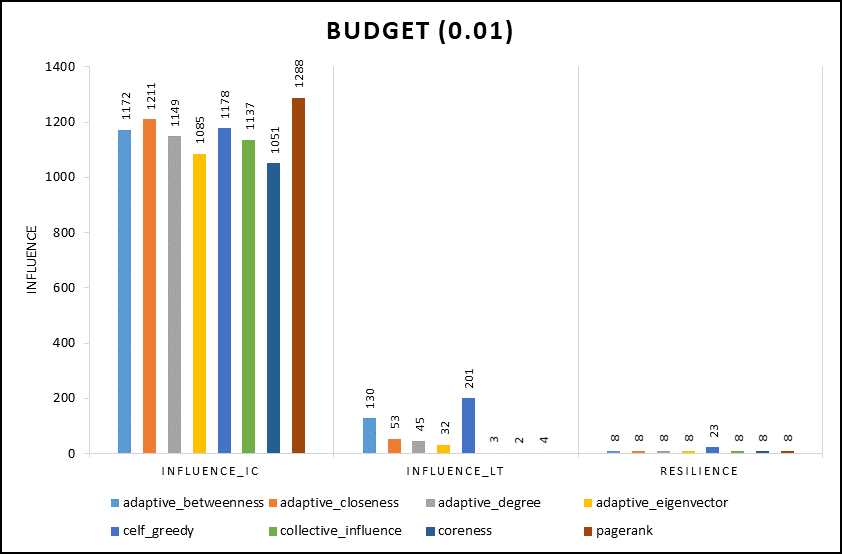
\includegraphics[angle=90, scale=0.65]{fb_johnshopkins-budget-1}\par 
				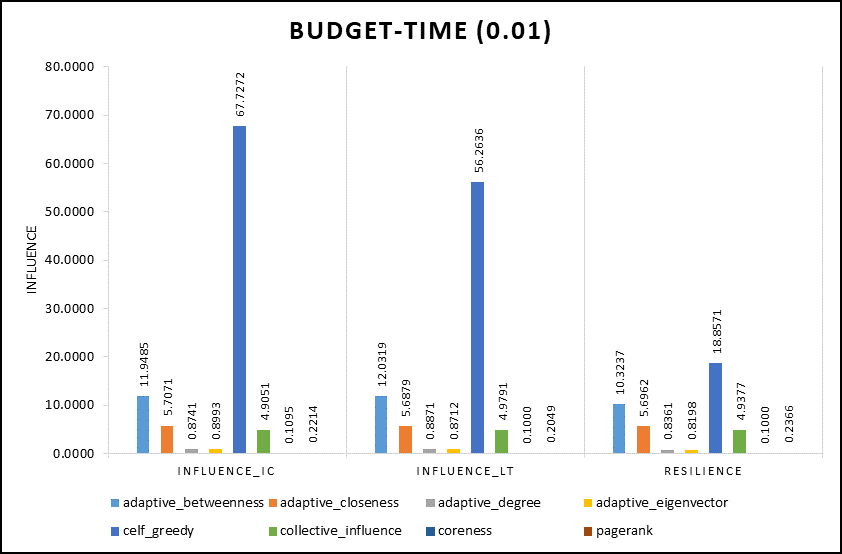
\includegraphics[angle=90, scale=0.65]{fb_johnshopkins-budget-time-1}\par 
			\end{multicols}
			\begin{multicols}{2}
				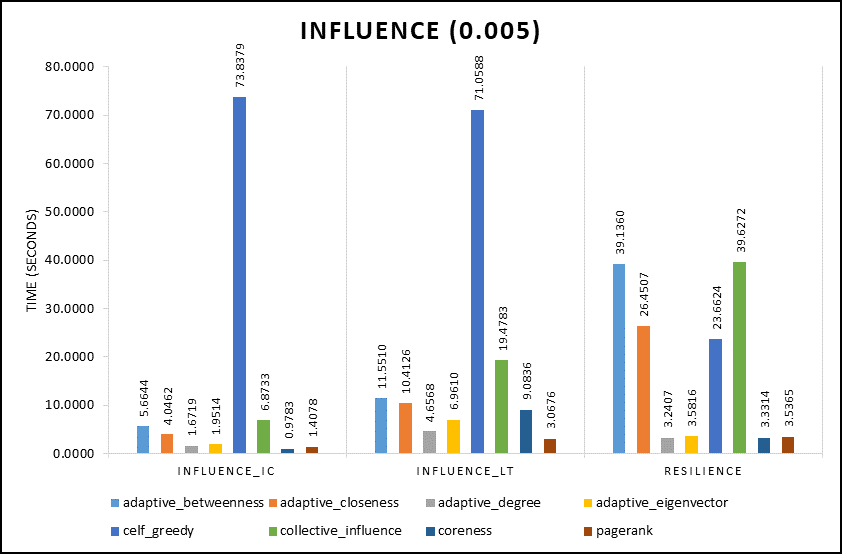
\includegraphics[angle=90, scale=0.65]{fb_johnshopkins-influence-1}\par 
			\end{multicols}
			
			\caption{Influence measure (top-left), normalized elapsed time for budget criteria (top-right), and normalized elapsed time for influence criteria (bottom-left) of Facebook - Johns Hopkins network.}
			\label{fig:inf-framework-fb_johnshopkins}
		\end{figure*}
		
		
		% *** fb_tvshows ***
		\begin{figure*}[ht]
			\begin{multicols}{2}
				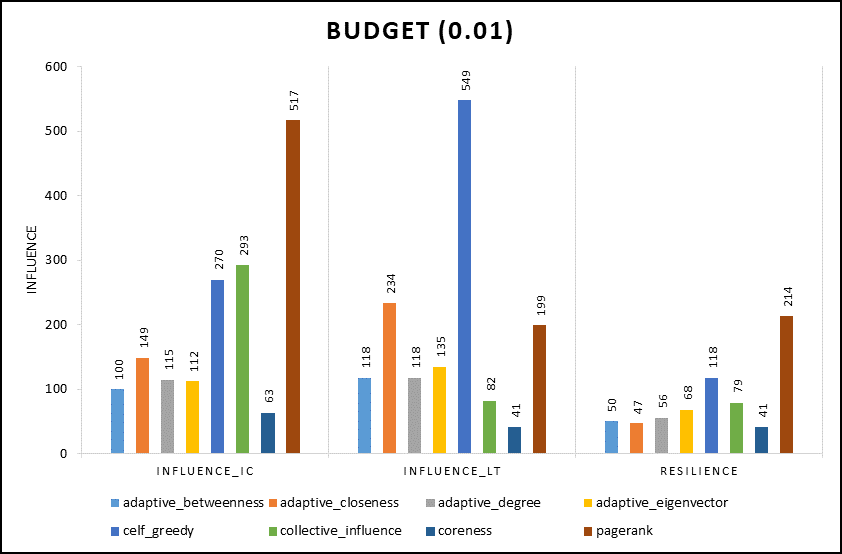
\includegraphics[angle=90, scale=0.65]{fb_tvshows-budget-1}\par 
				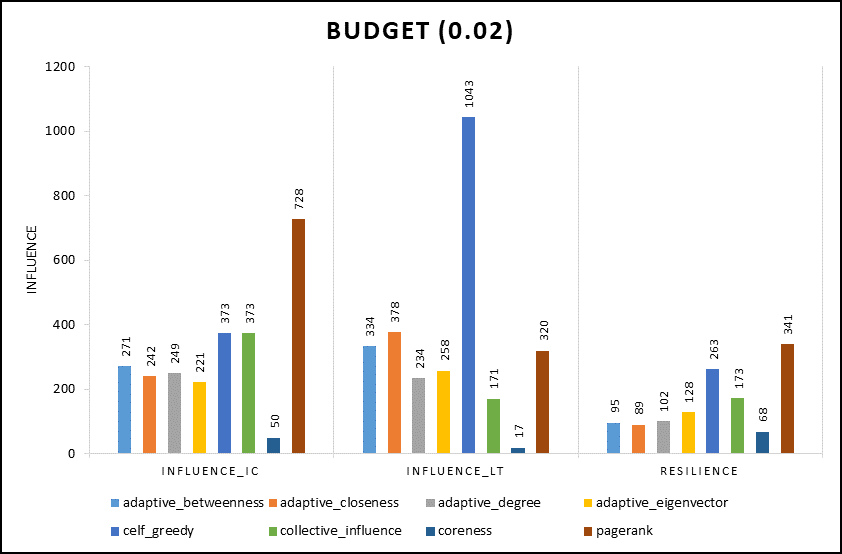
\includegraphics[angle=90, scale=0.65]{fb_tvshows-budget-2}\par 
			\end{multicols}
			\begin{multicols}{2}
				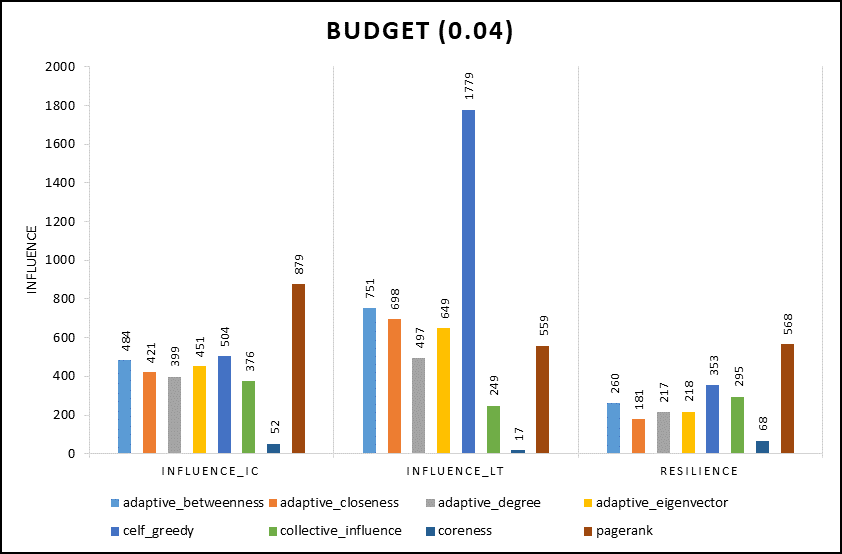
\includegraphics[angle=90, scale=0.65]{fb_tvshows-budget-4}\par 
				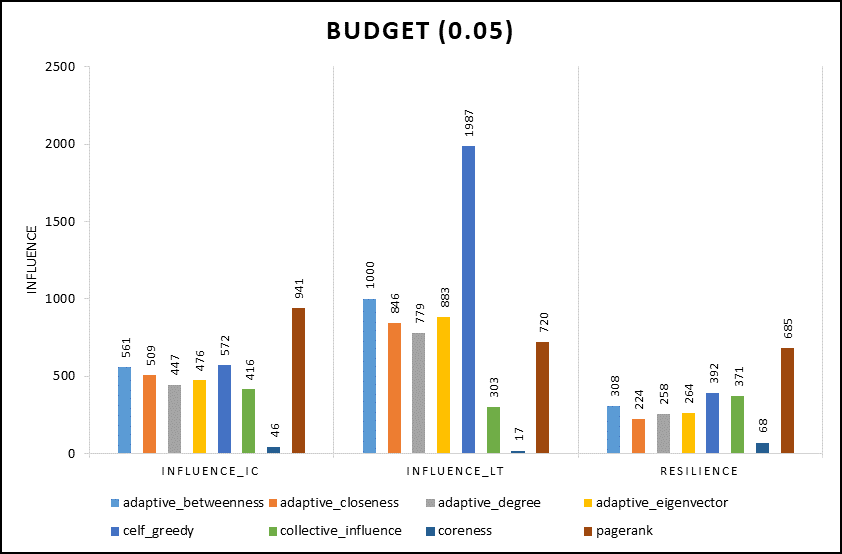
\includegraphics[angle=90, scale=0.65]{fb_tvshows-budget-5}\par 
			\end{multicols}
			
			\caption{Influence measure of Facebook - TV Shows network on range on all budgets evaluated for all three tests.}
			\label{fig:inf-framework-fb_tvshows}
		\end{figure*}
		
		\begin{figure*}[ht]
			\begin{multicols}{2}
				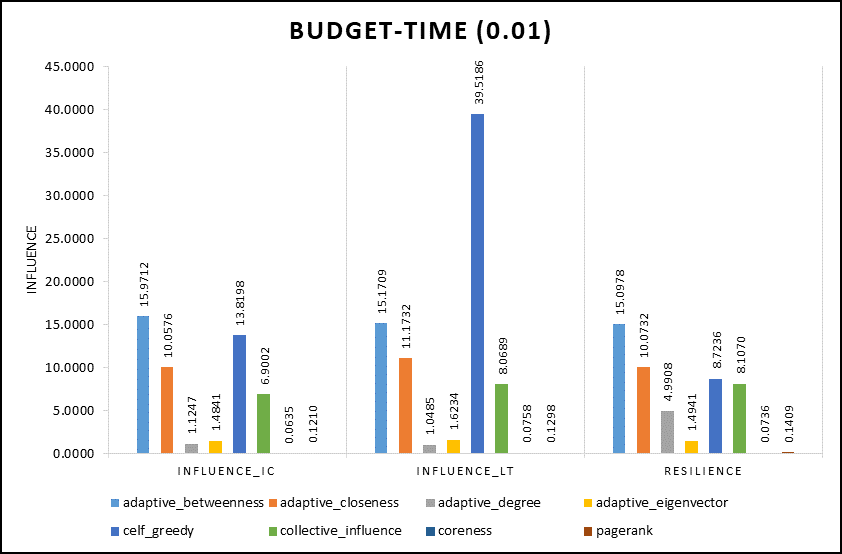
\includegraphics[angle=90, scale=0.65]{fb_tvshows-budget-time-1}\par 
				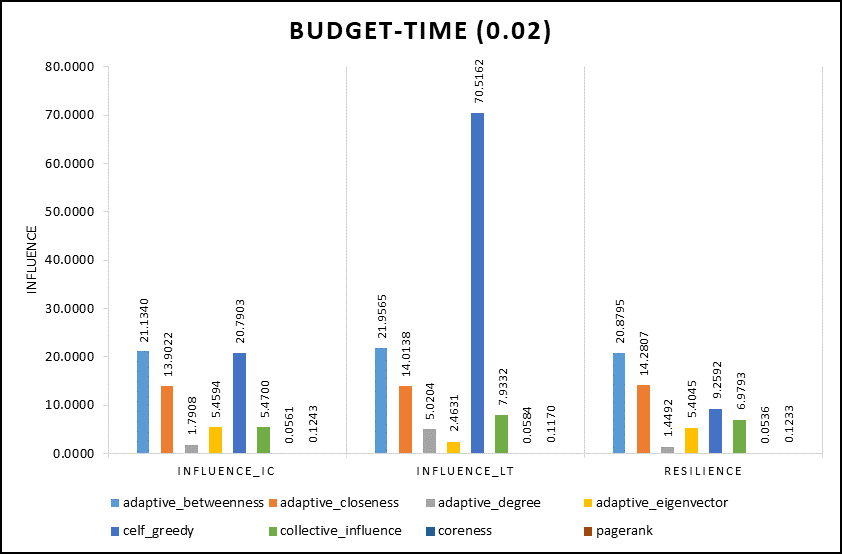
\includegraphics[angle=90, scale=0.65]{fb_tvshows-budget-time-2}\par 
			\end{multicols}
			\begin{multicols}{2}
				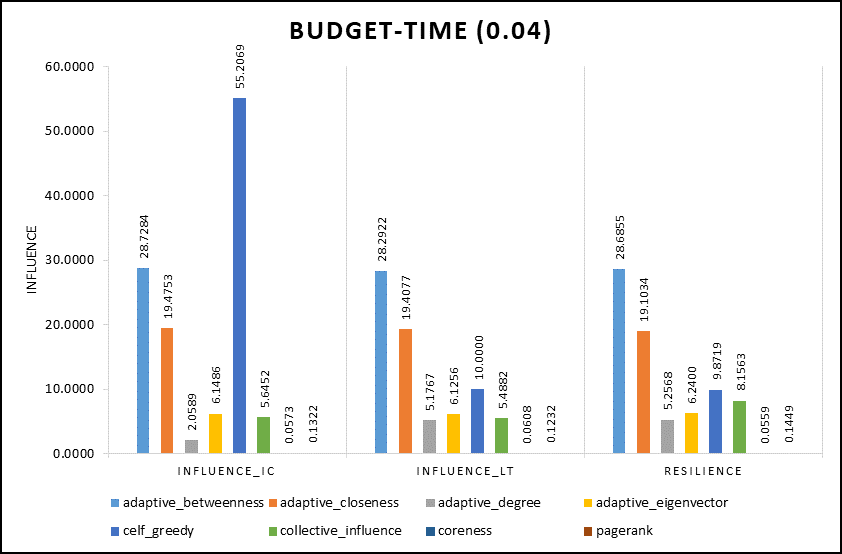
\includegraphics[angle=90, scale=0.65]{fb_tvshows-budget-time-4}\par 
				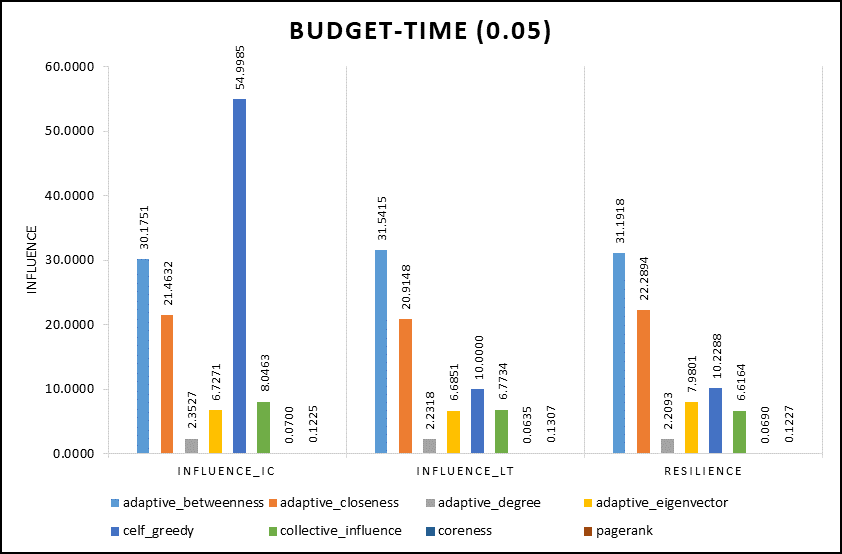
\includegraphics[angle=90, scale=0.65]{fb_tvshows-budget-time-5}\par 
			\end{multicols}
			
			\caption{Normalized elapsed time for budget criteria on Facebook - TV Shows network.}
			\label{fig:inf-framework-fb_tvshows2}
		\end{figure*}
		
		\begin{figure*}[h]
			\begin{multicols}{2}
				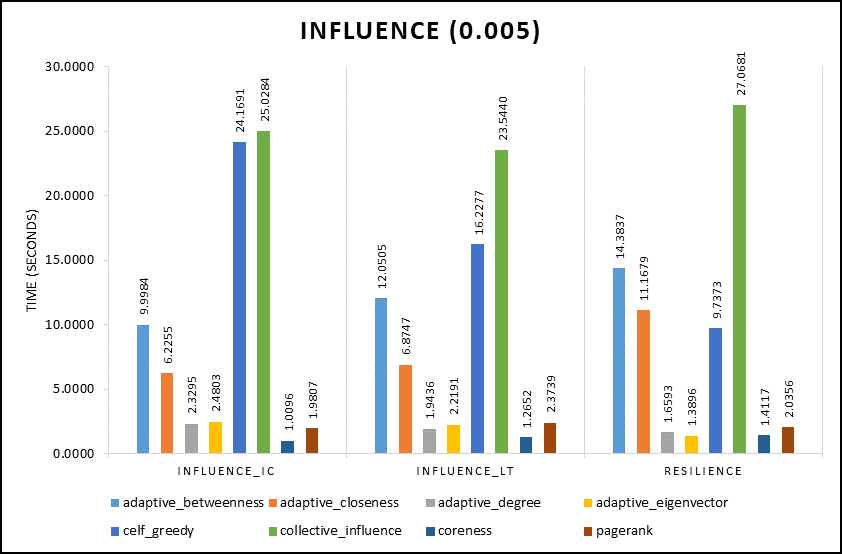
\includegraphics[angle=90, scale=0.65]{fb_tvshows-influence-1}\par 
				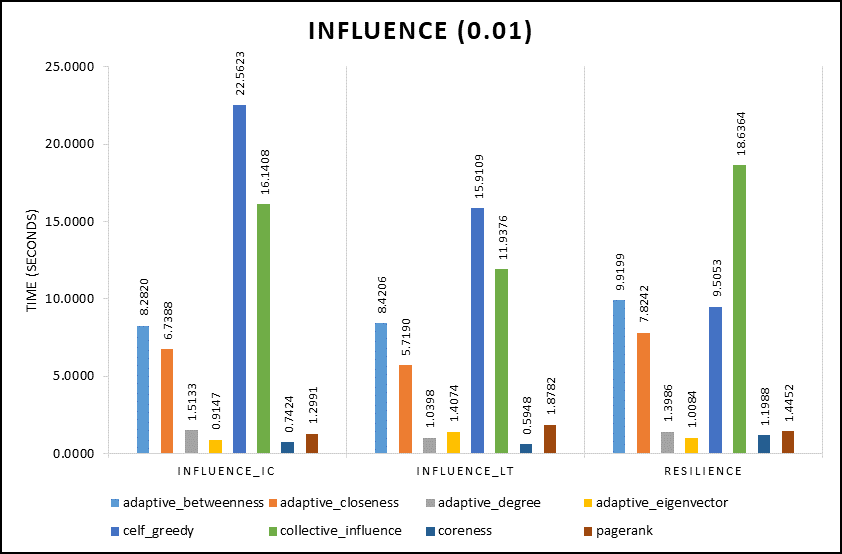
\includegraphics[angle=90, scale=0.65]{fb_tvshows-influence-2}\par 
			\end{multicols}
			\begin{multicols}{2}
				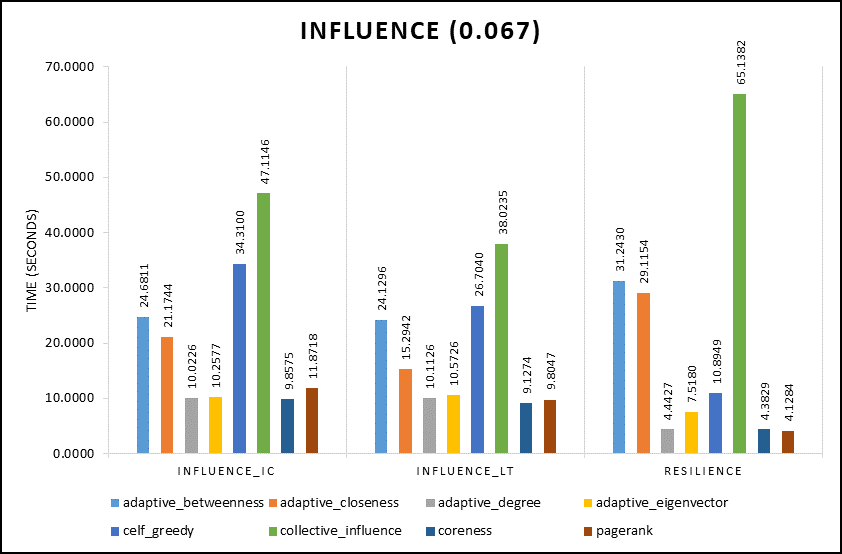
\includegraphics[angle=90, scale=0.65]{fb_tvshows-influence-4}\par 
				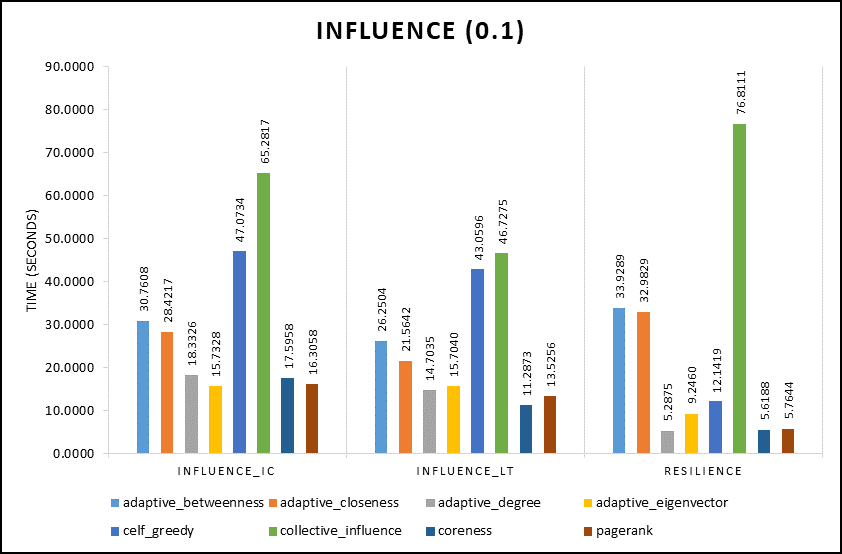
\includegraphics[angle=90, scale=0.65]{fb_tvshows-influence-5}\par 
			\end{multicols}
			
			\caption{Normalized elapsed time for influence criteria on Facebook - TV Shows network.}
			\label{fig:inf-framework-fb_tvshows3}
		\end{figure*}
		
		
		% *** football ***
		\begin{figure*}[ht]
			\begin{multicols}{2}
				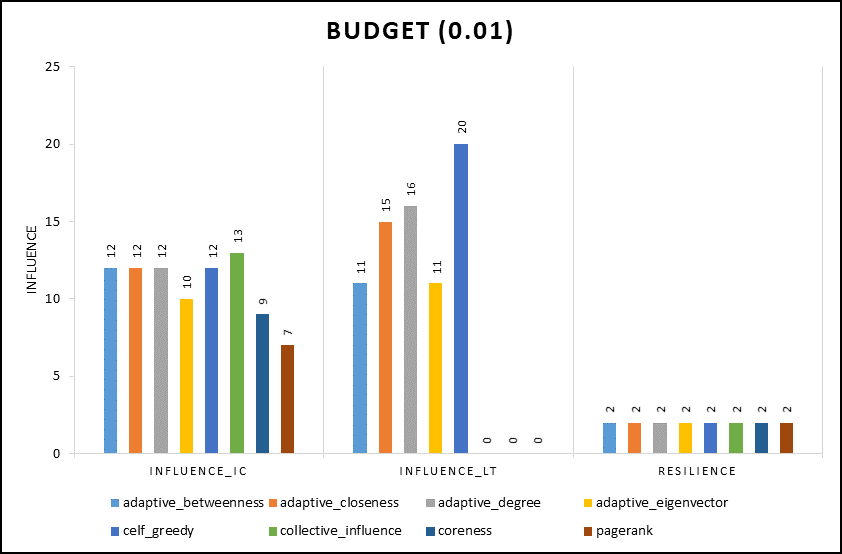
\includegraphics[angle=90, scale=0.65]{football-budget-1}\par 
				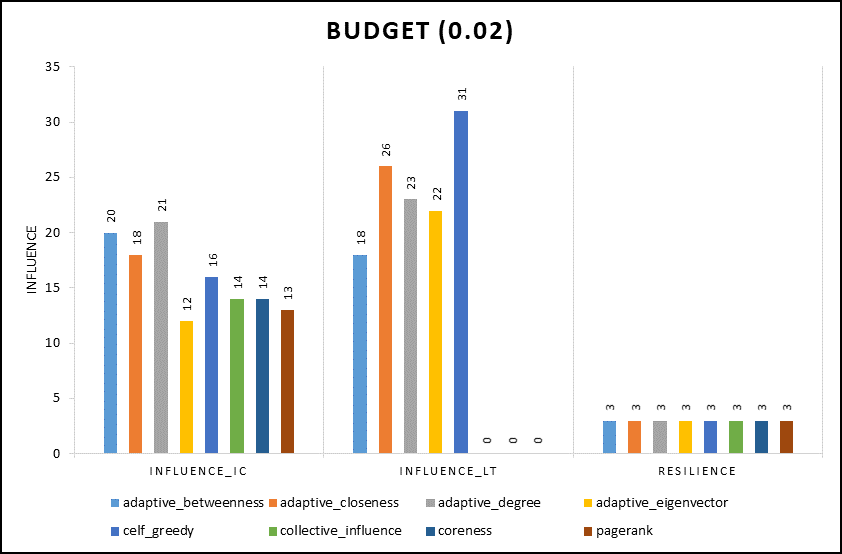
\includegraphics[angle=90, scale=0.65]{football-budget-2}\par 
			\end{multicols}
			\begin{multicols}{2}
				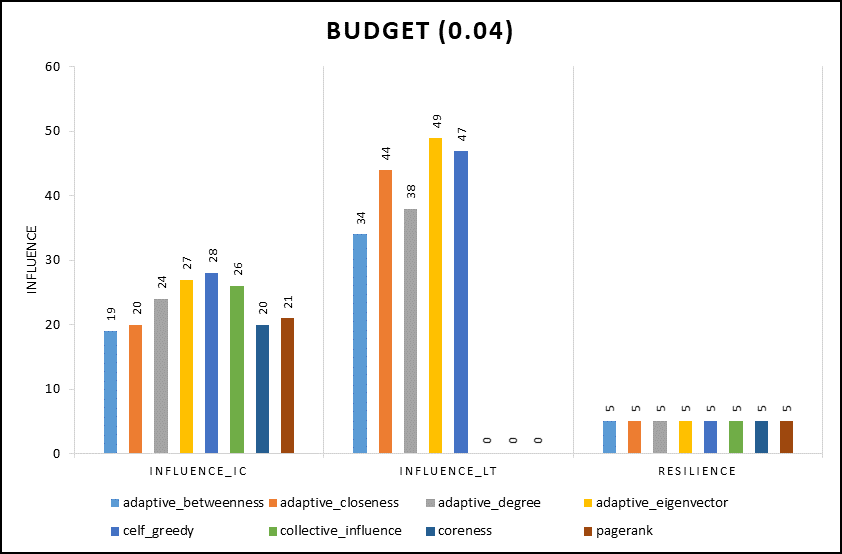
\includegraphics[angle=90, scale=0.65]{football-budget-4}\par 
				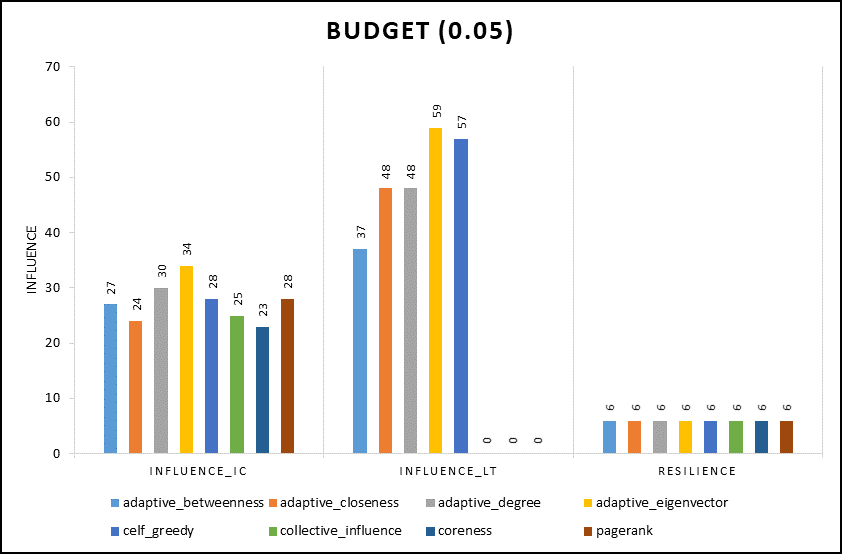
\includegraphics[angle=90, scale=0.65]{football-budget-5}\par 
			\end{multicols}
			
			\caption{Influence measure of Football network on range on all budgets evaluated for all three tests.}
			\label{fig:inf-framework-football}
		\end{figure*}
		
		\begin{figure*}[ht]
			\begin{multicols}{2}
				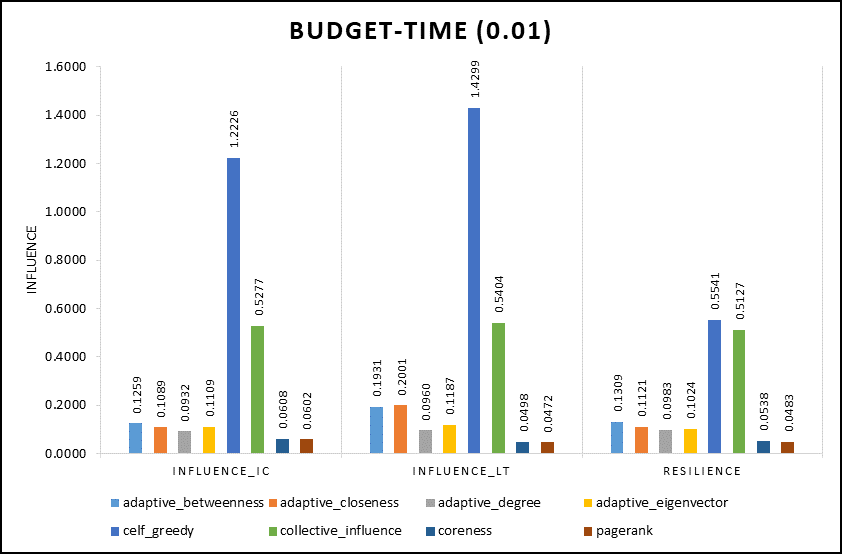
\includegraphics[angle=90, scale=0.65]{football-budget-time-1}\par 
				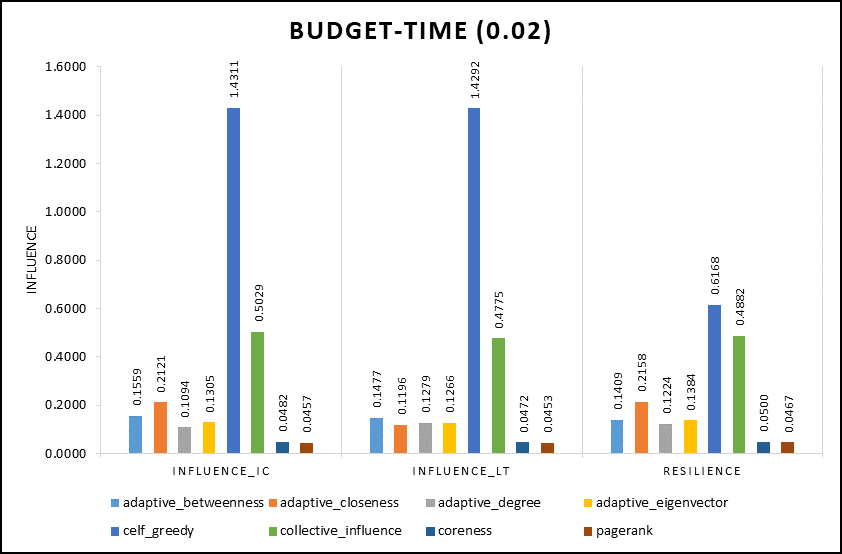
\includegraphics[angle=90, scale=0.65]{football-budget-time-2}\par 
			\end{multicols}
			\begin{multicols}{2}
				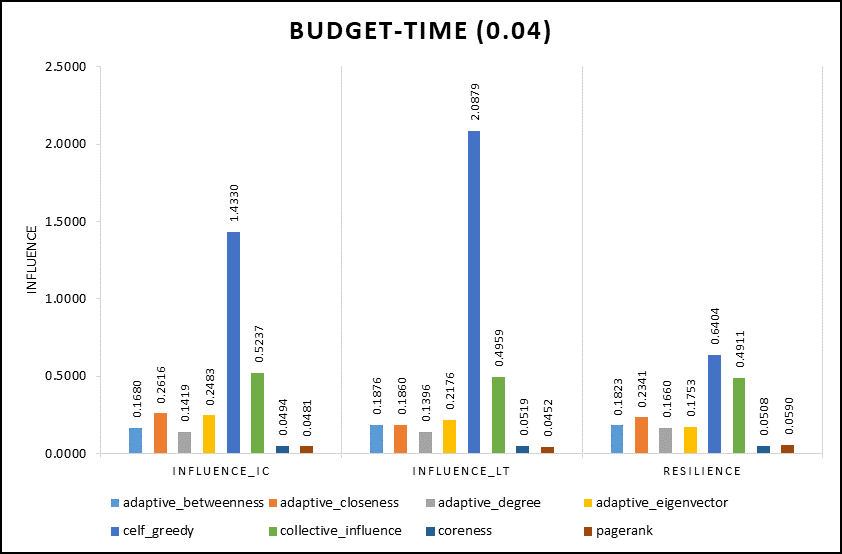
\includegraphics[angle=90, scale=0.65]{football-budget-time-4}\par 
				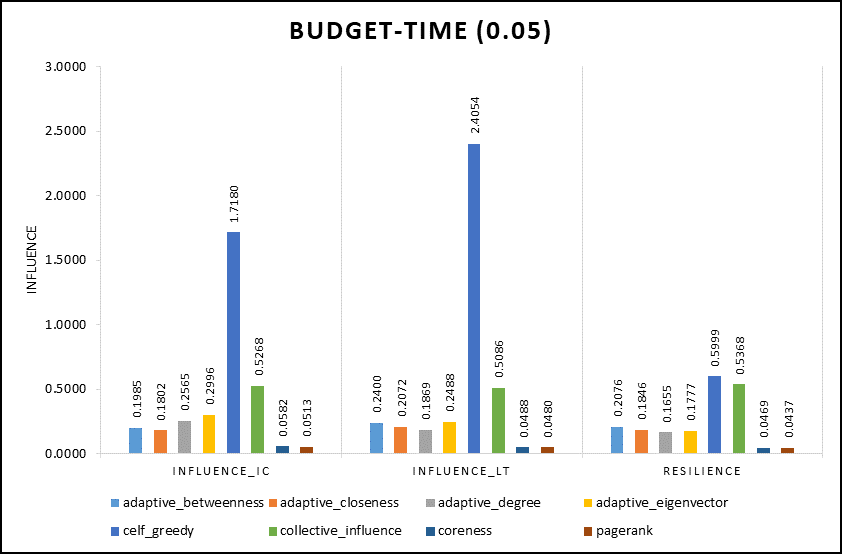
\includegraphics[angle=90, scale=0.65]{football-budget-time-5}\par 
			\end{multicols}
			
			\caption{Normalized elapsed time for budget criteria on Football network.}
			\label{fig:inf-framework-football2}
		\end{figure*}
		
		\begin{figure*}[h]
			\begin{multicols}{2}
				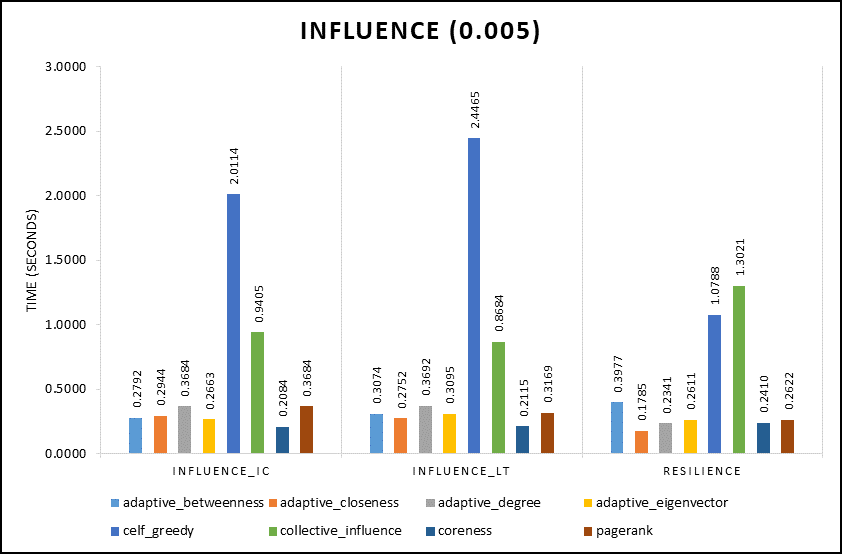
\includegraphics[angle=90, scale=0.65]{football-influence-1}\par 
				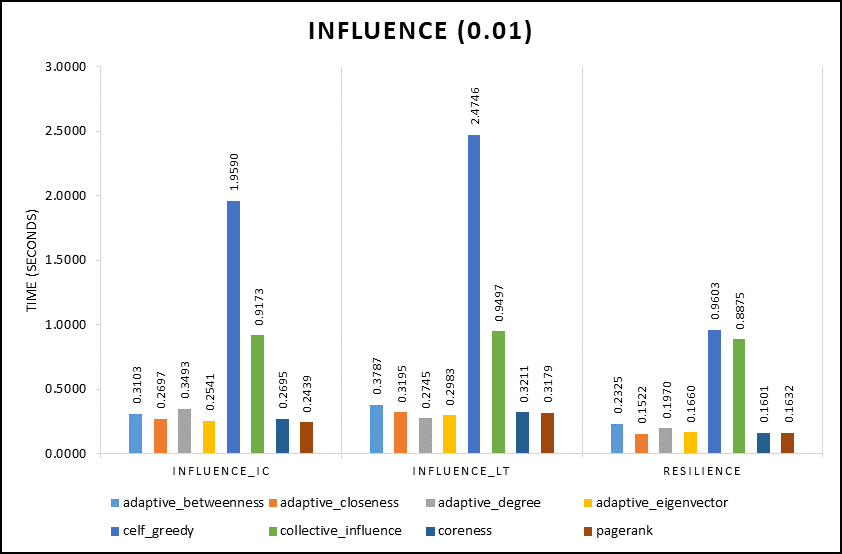
\includegraphics[angle=90, scale=0.65]{football-influence-2}\par 
			\end{multicols}
			\begin{multicols}{2}
				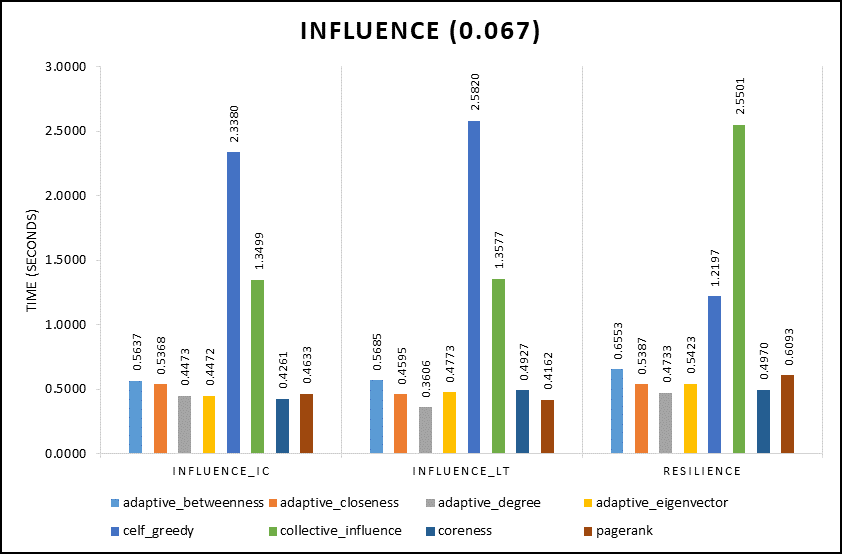
\includegraphics[angle=90, scale=0.65]{football-influence-4}\par 
				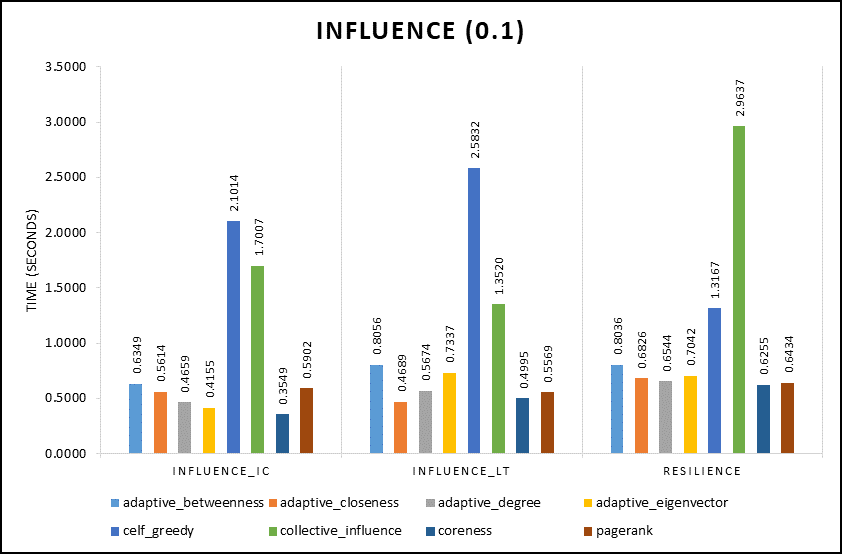
\includegraphics[angle=90, scale=0.65]{football-influence-5}\par 
			\end{multicols}
			
			\caption{Normalized elapsed time for influence criteria on Football network.}
			\label{fig:inf-framework-football3}
		\end{figure*}
		
		
		% *** hamster ***
		\begin{figure*}[ht]
			\begin{multicols}{2}
				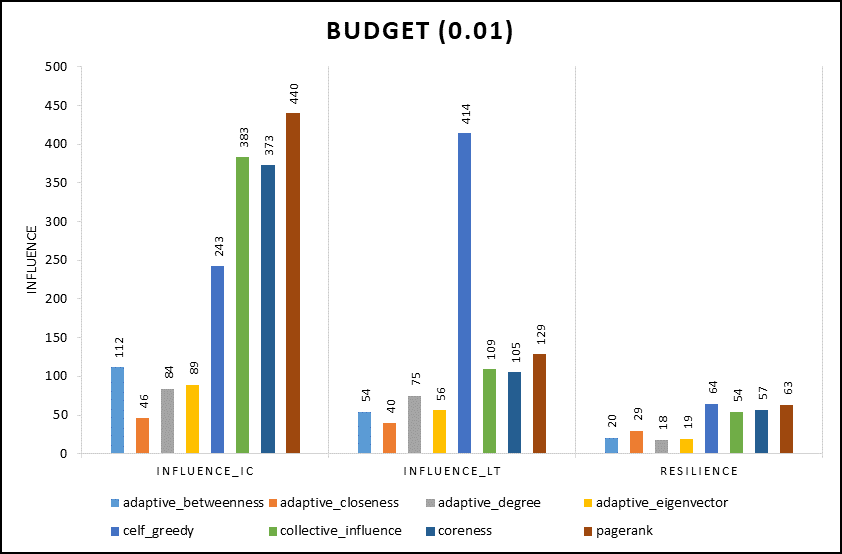
\includegraphics[angle=90, scale=0.65]{hamster-budget-1}\par 
				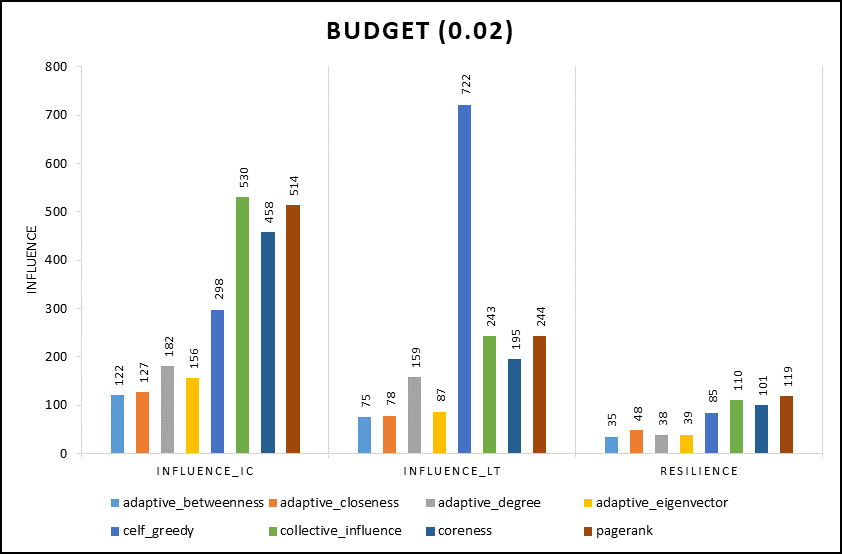
\includegraphics[angle=90, scale=0.65]{hamster-budget-2}\par 
			\end{multicols}
			\begin{multicols}{2}
				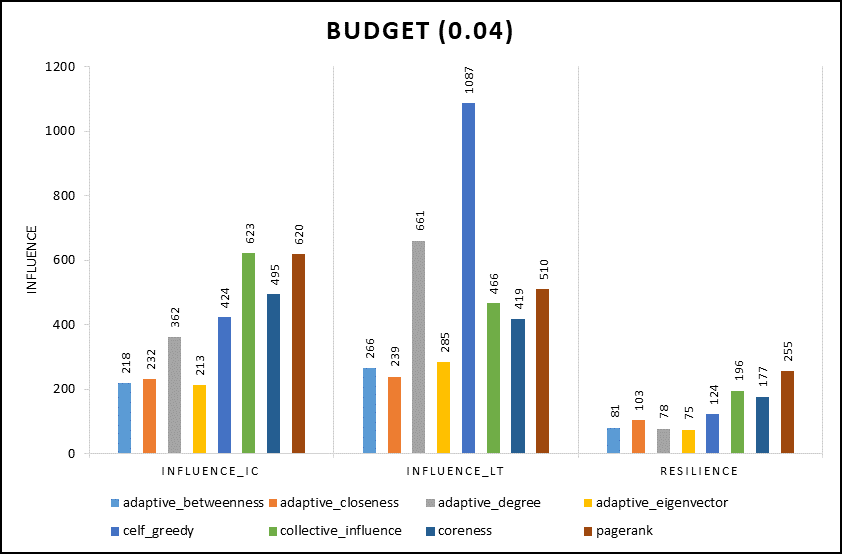
\includegraphics[angle=90, scale=0.65]{hamster-budget-4}\par 
				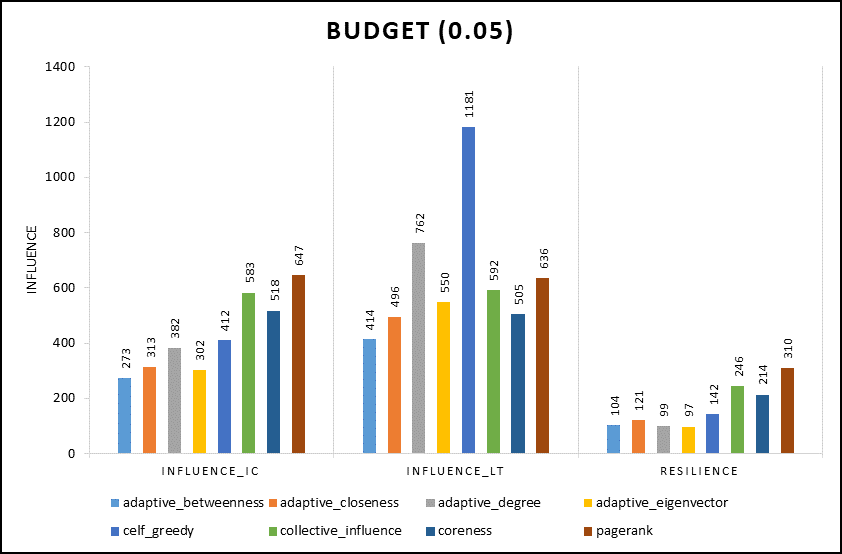
\includegraphics[angle=90, scale=0.65]{hamster-budget-5}\par 
			\end{multicols}
			
			\caption{Influence measure of hamster network on range on all budgets evaluated for all three tests.}
			\label{fig:inf-framework-hamster}
		\end{figure*}
		
		\begin{figure*}[ht]
			\begin{multicols}{2}
				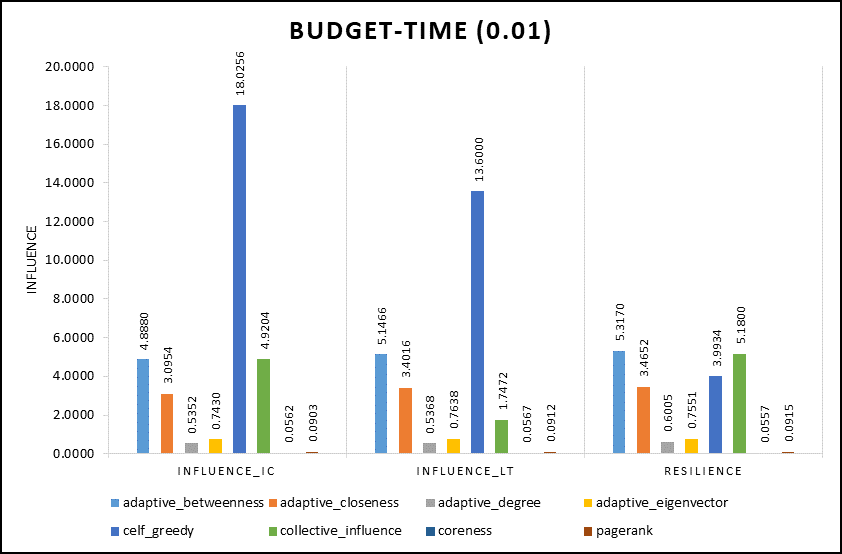
\includegraphics[angle=90, scale=0.65]{hamster-budget-time-1}\par 
				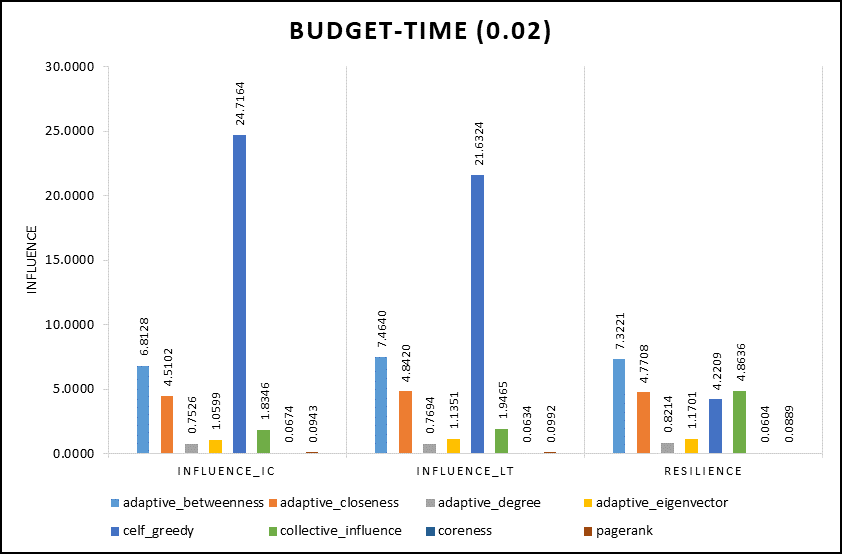
\includegraphics[angle=90, scale=0.65]{hamster-budget-time-2}\par 
			\end{multicols}
			\begin{multicols}{2}
				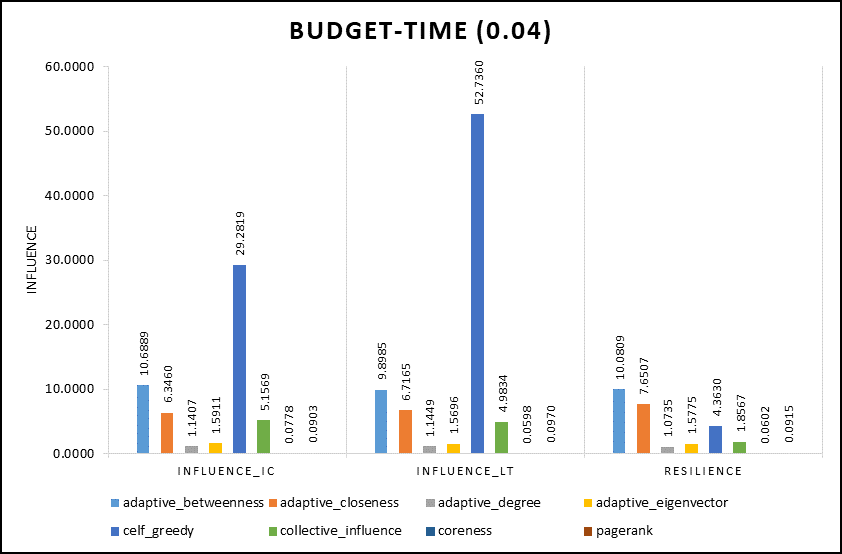
\includegraphics[angle=90, scale=0.65]{hamster-budget-time-4}\par 
				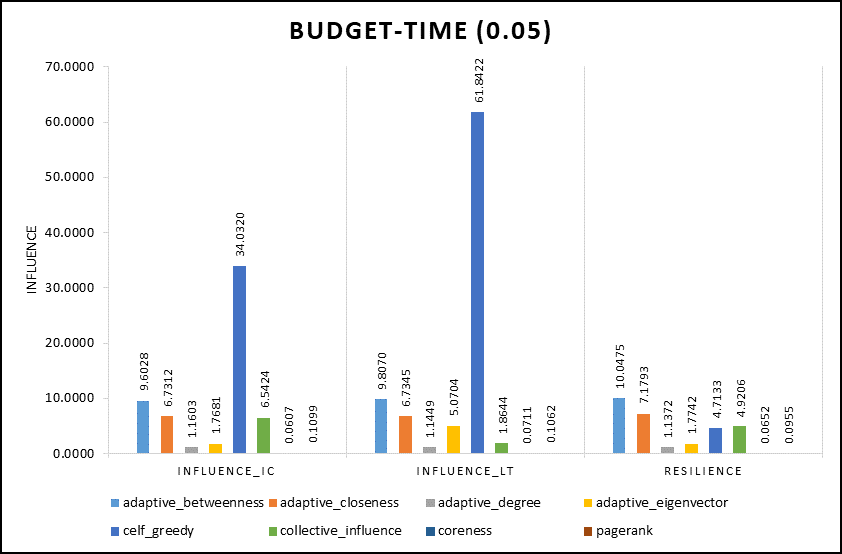
\includegraphics[angle=90, scale=0.65]{hamster-budget-time-5}\par 
			\end{multicols}
			
			\caption{Normalized elapsed time for budget criteria on hamster network.}
			\label{fig:inf-framework-hamster2}
		\end{figure*}
		
		\begin{figure*}[h]
			\begin{multicols}{2}
				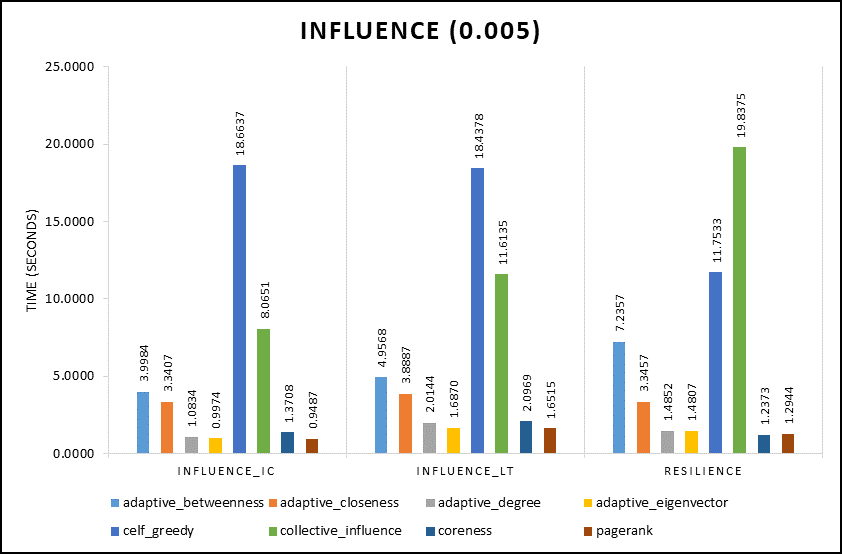
\includegraphics[angle=90, scale=0.65]{hamster-influence-1}\par 
				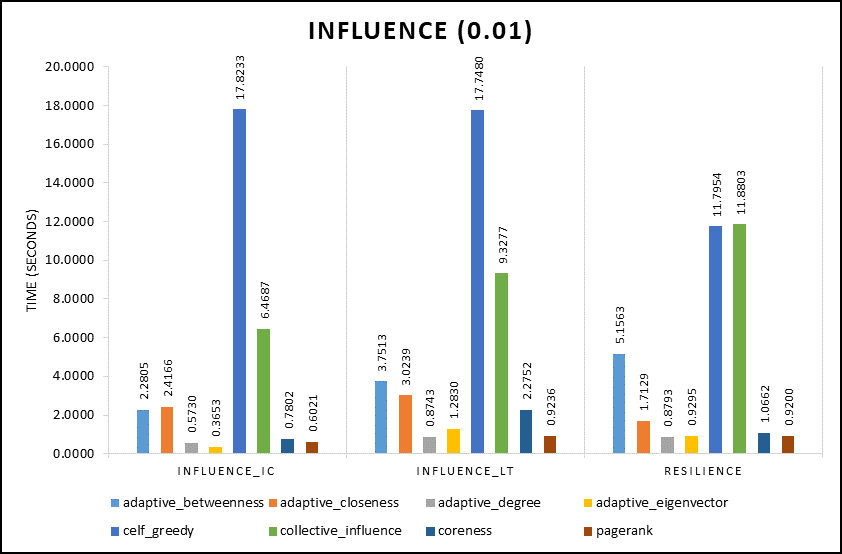
\includegraphics[angle=90, scale=0.65]{hamster-influence-2}\par 
			\end{multicols}
			\begin{multicols}{2}
				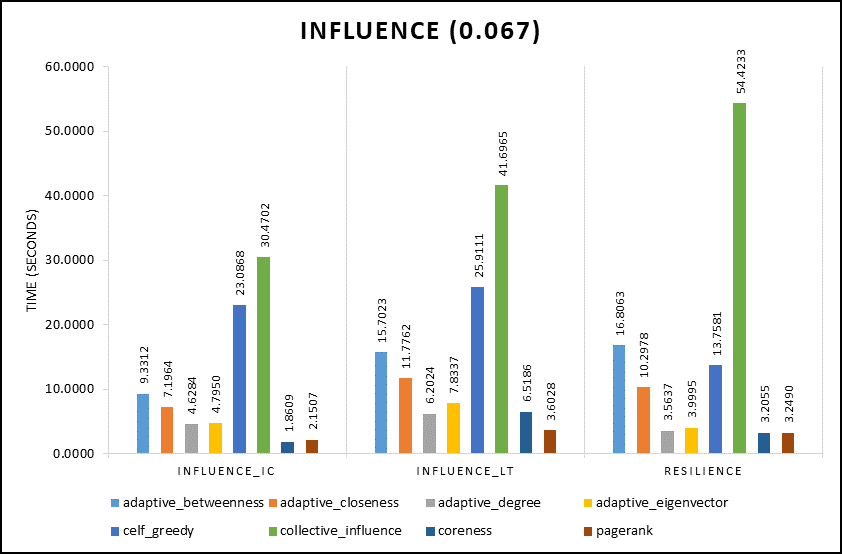
\includegraphics[angle=90, scale=0.65]{hamster-influence-4}\par 
				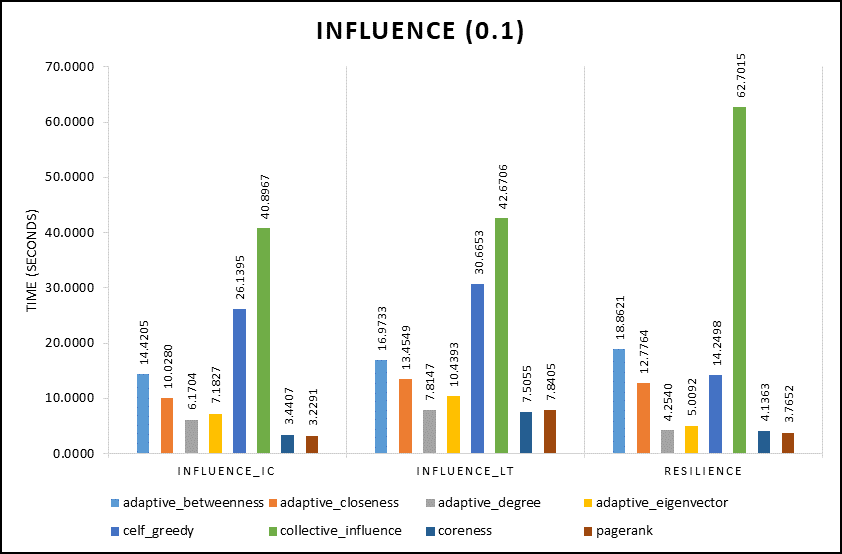
\includegraphics[angle=90, scale=0.65]{hamster-influence-5}\par 
			\end{multicols}
			
			\caption{Normalized elapsed time for influence criteria on hamster network.}
			\label{fig:inf-framework-hamster3}
		\end{figure*}
		
		
		% *** influence_citation ***
		\begin{figure*}[ht]
			\begin{multicols}{2}
				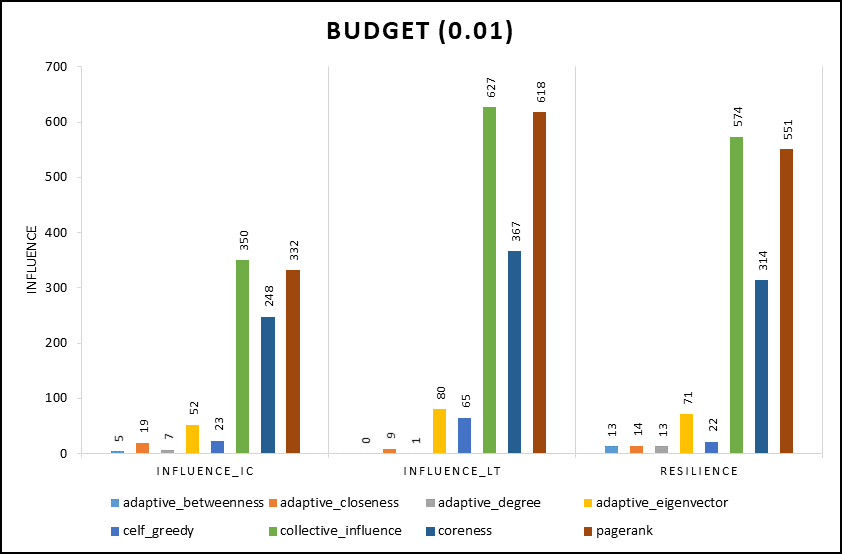
\includegraphics[angle=90, scale=0.65]{influence_citation-budget-1}\par 
				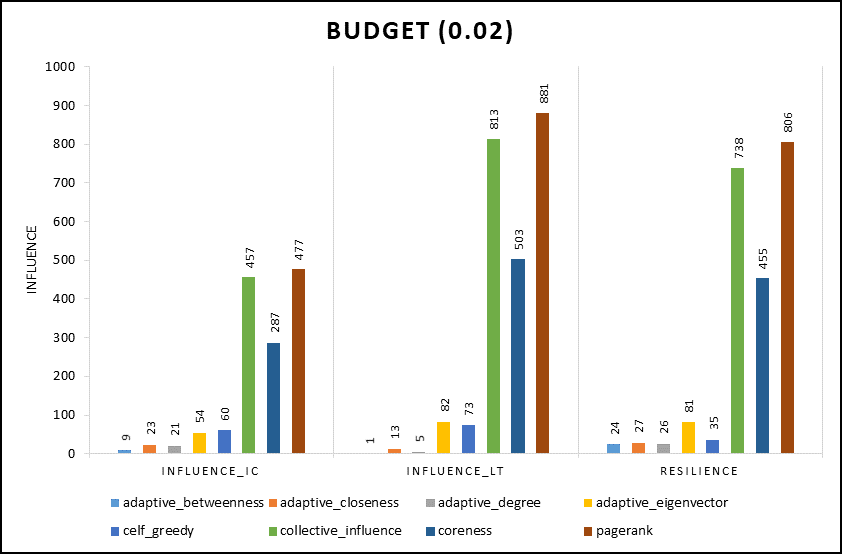
\includegraphics[angle=90, scale=0.65]{influence_citation-budget-2}\par 
			\end{multicols}
			\begin{multicols}{2}
				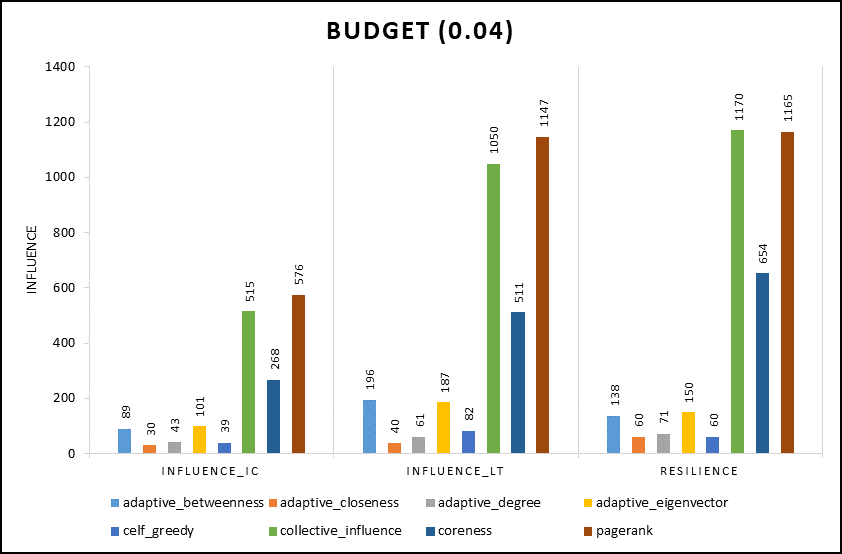
\includegraphics[angle=90, scale=0.65]{influence_citation-budget-4}\par 
				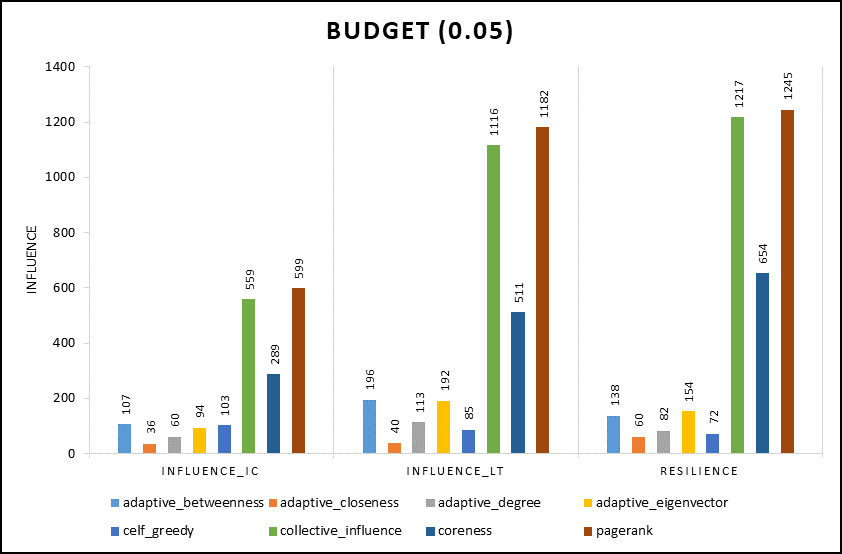
\includegraphics[angle=90, scale=0.65]{influence_citation-budget-5}\par 
			\end{multicols}
			
			\caption{Influence measure of Citation network of influence mining papers network on range on all budgets evaluated for all three tests.}
			\label{fig:inf-framework-influence_citation}
		\end{figure*}
		
		\begin{figure*}[ht]
			\begin{multicols}{2}
				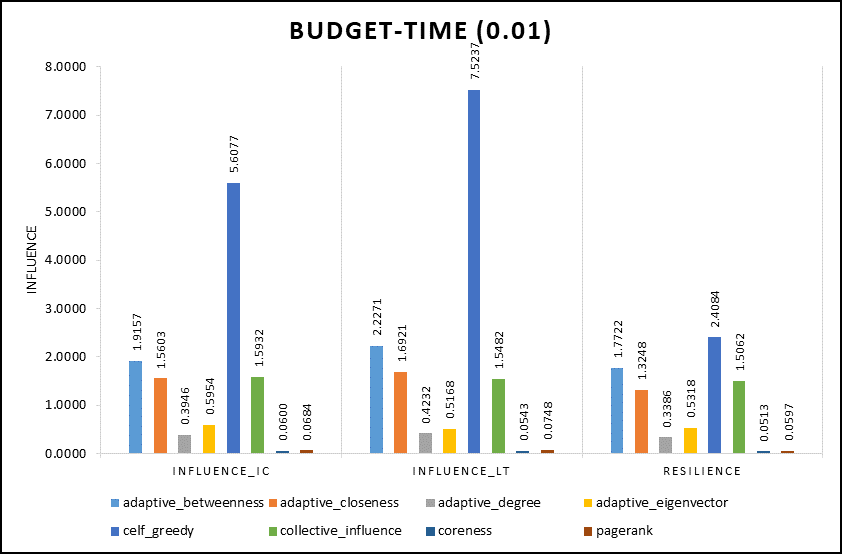
\includegraphics[angle=90, scale=0.65]{influence_citation-budget-time-1}\par 
				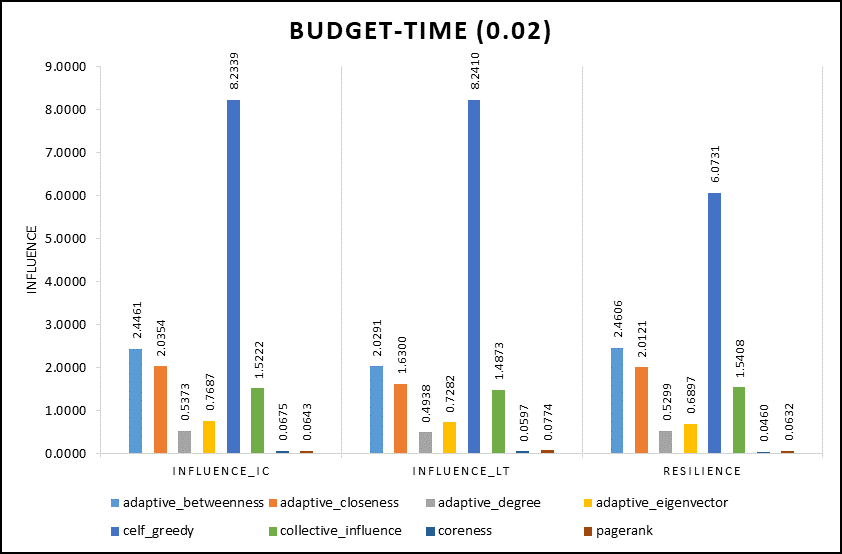
\includegraphics[angle=90, scale=0.65]{influence_citation-budget-time-2}\par 
			\end{multicols}
			\begin{multicols}{2}
				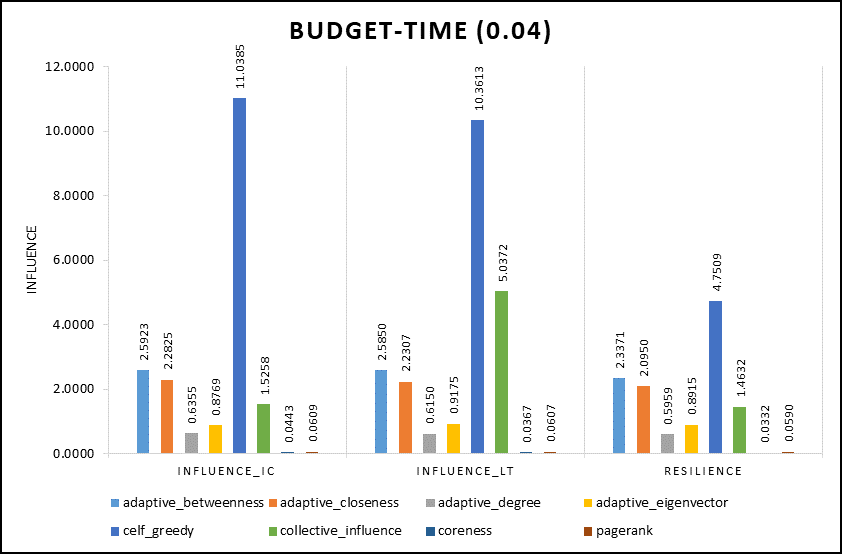
\includegraphics[angle=90, scale=0.65]{influence_citation-budget-time-4}\par 
				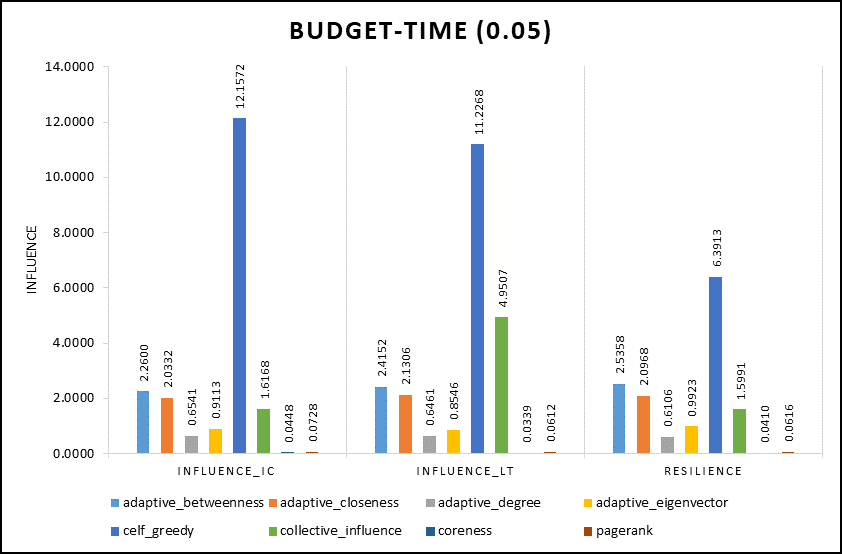
\includegraphics[angle=90, scale=0.65]{influence_citation-budget-time-5}\par 
			\end{multicols}
			
			\caption{Normalized elapsed time for budget criteria on Citation network of influence mining papers.}
			\label{fig:inf-framework-influence_citation2}
		\end{figure*}
		
		\begin{figure*}[h]
			\begin{multicols}{2}
				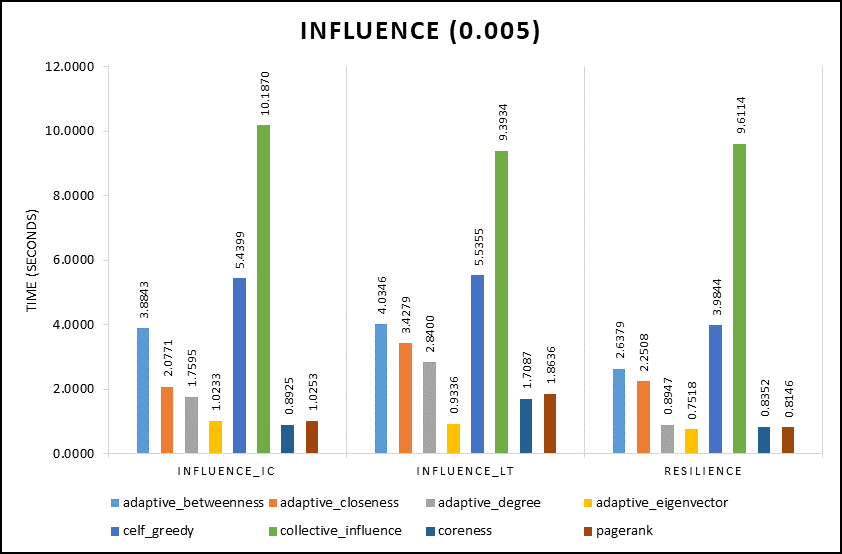
\includegraphics[angle=90, scale=0.65]{influence_citation-influence-1}\par 
				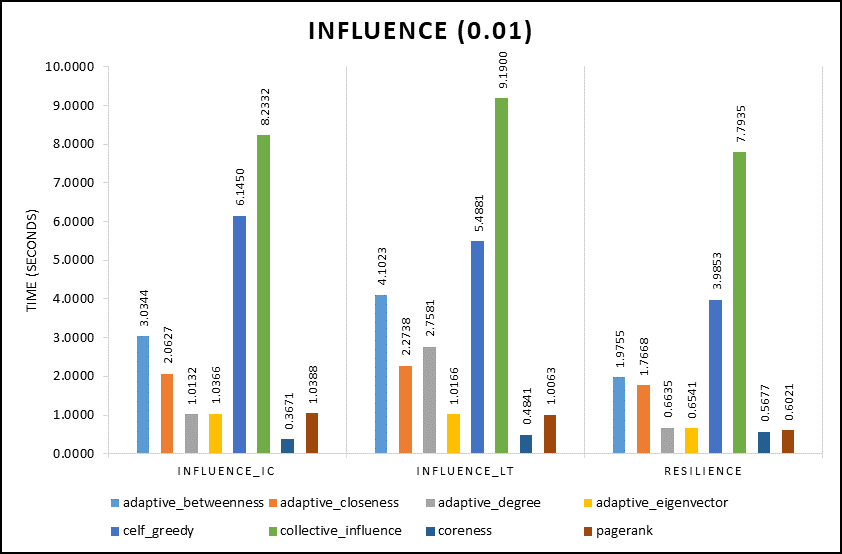
\includegraphics[angle=90, scale=0.65]{influence_citation-influence-2}\par 
			\end{multicols}
			\begin{multicols}{2}
				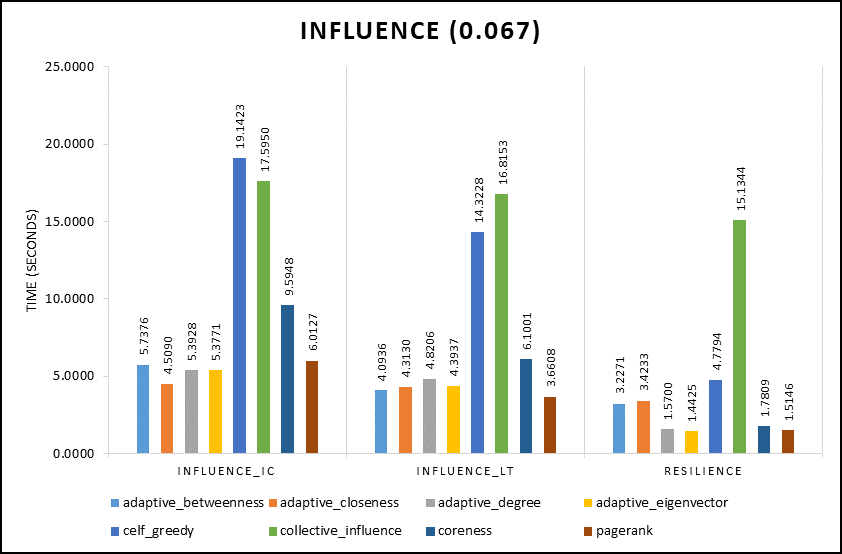
\includegraphics[angle=90, scale=0.65]{influence_citation-influence-4}\par 
				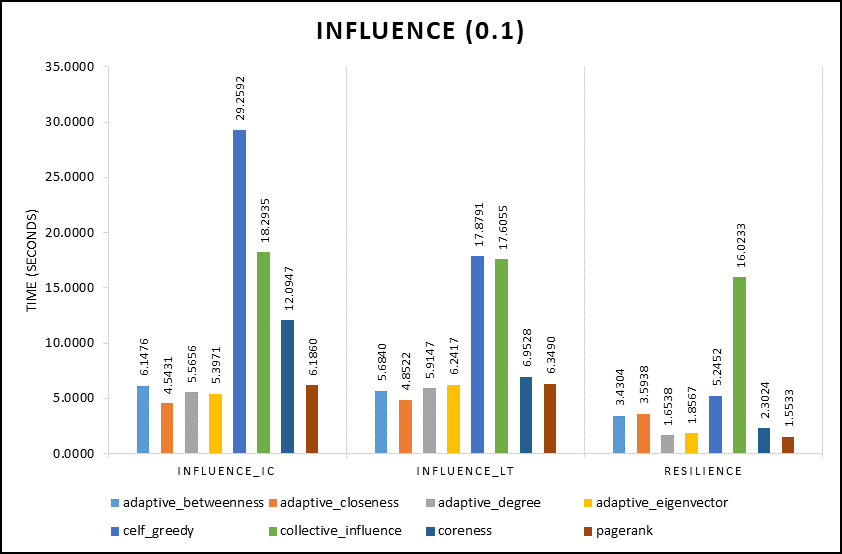
\includegraphics[angle=90, scale=0.65]{influence_citation-influence-5}\par 
			\end{multicols}
			
			\caption{Normalized elapsed time for influence criteria on Citation network of influence mining papers.}
			\label{fig:inf-framework-influence_citation3}
		\end{figure*}
		
		
		% *** ita2000 ***
		\begin{figure*}[ht]
			\begin{multicols}{2}
				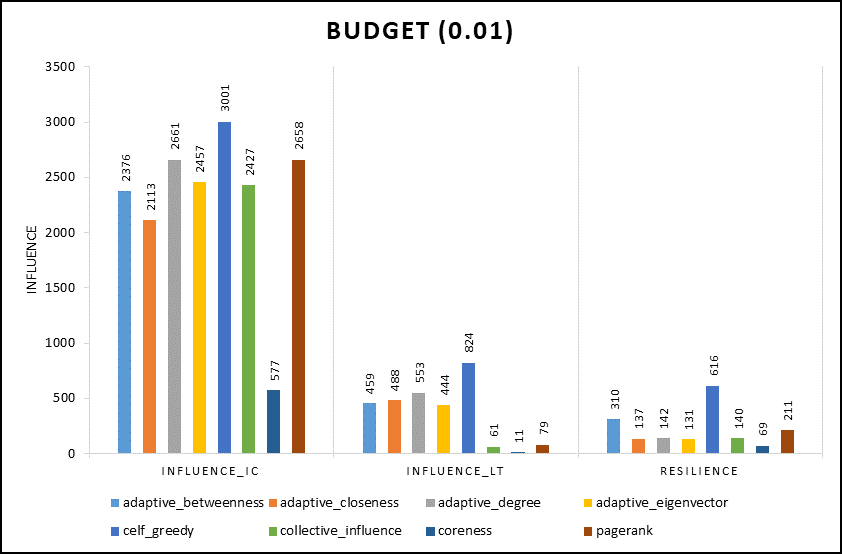
\includegraphics[angle=90, scale=0.65]{ita2000-budget-1}\par 
				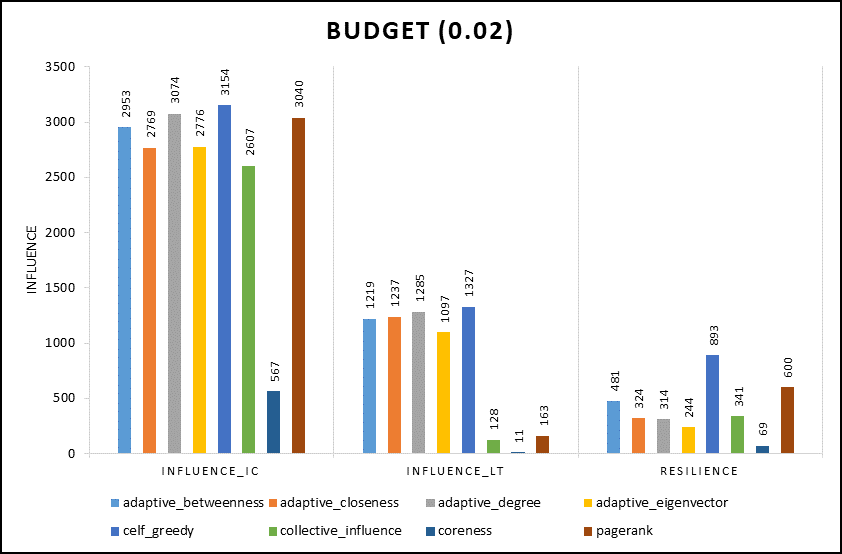
\includegraphics[angle=90, scale=0.65]{ita2000-budget-2}\par 
			\end{multicols}
			\begin{multicols}{2}
				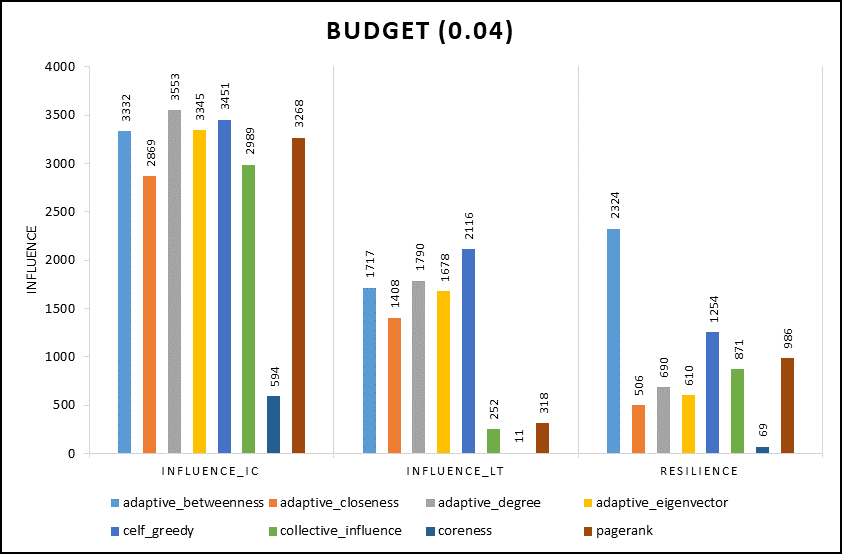
\includegraphics[angle=90, scale=0.65]{ita2000-budget-4}\par 
				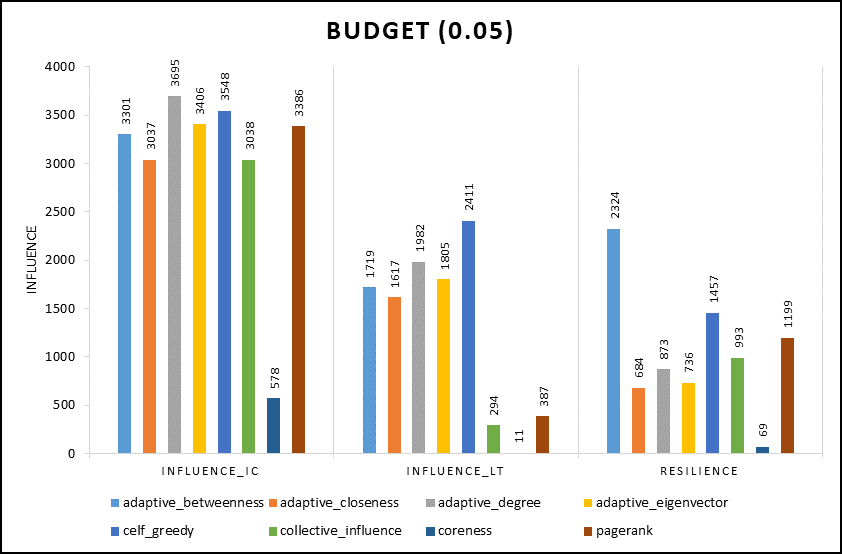
\includegraphics[angle=90, scale=0.65]{ita2000-budget-5}\par 
			\end{multicols}
			
			\caption{Influence measure of ITA-2000 network of influence mining papers network on range on all budgets evaluated for all three tests.}
			\label{fig:inf-framework-ita2000}
		\end{figure*}
		
		\begin{figure*}[ht]
			\begin{multicols}{2}
				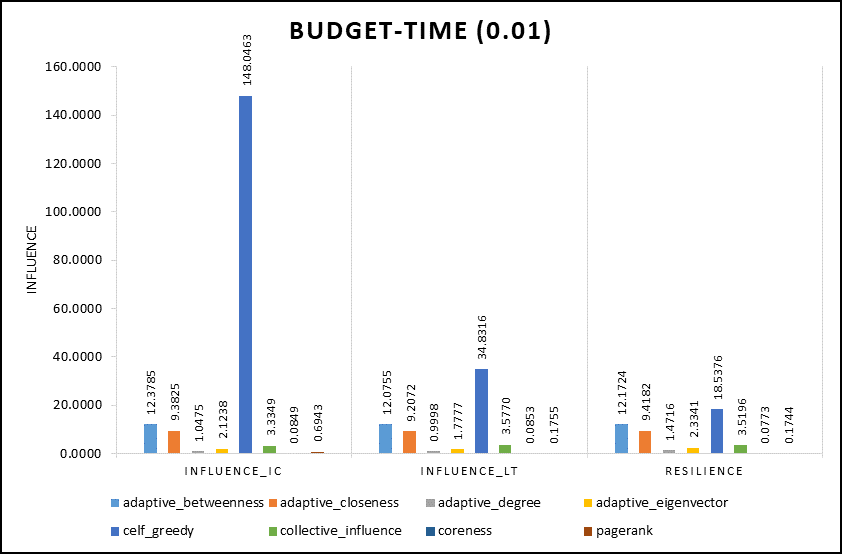
\includegraphics[angle=90, scale=0.65]{ita2000-budget-time-1}\par 
				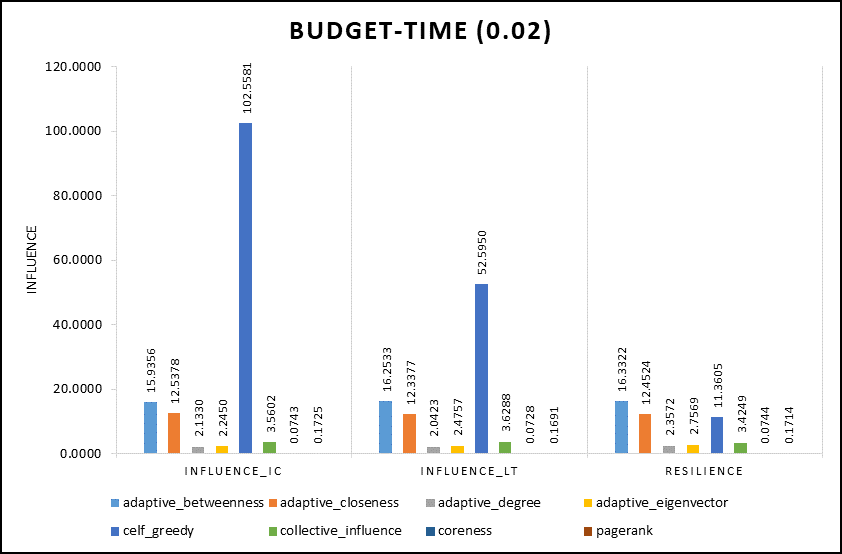
\includegraphics[angle=90, scale=0.65]{ita2000-budget-time-2}\par 
			\end{multicols}
			\begin{multicols}{2}
				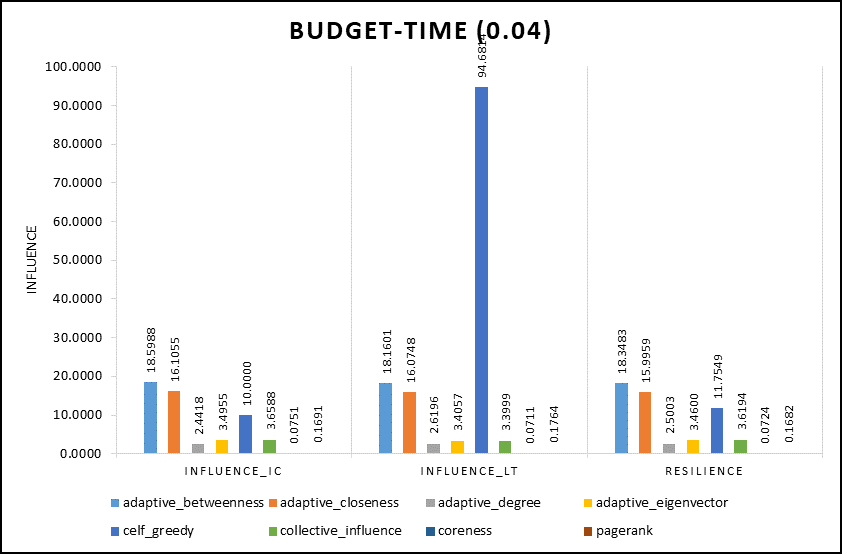
\includegraphics[angle=90, scale=0.65]{ita2000-budget-time-4}\par 
				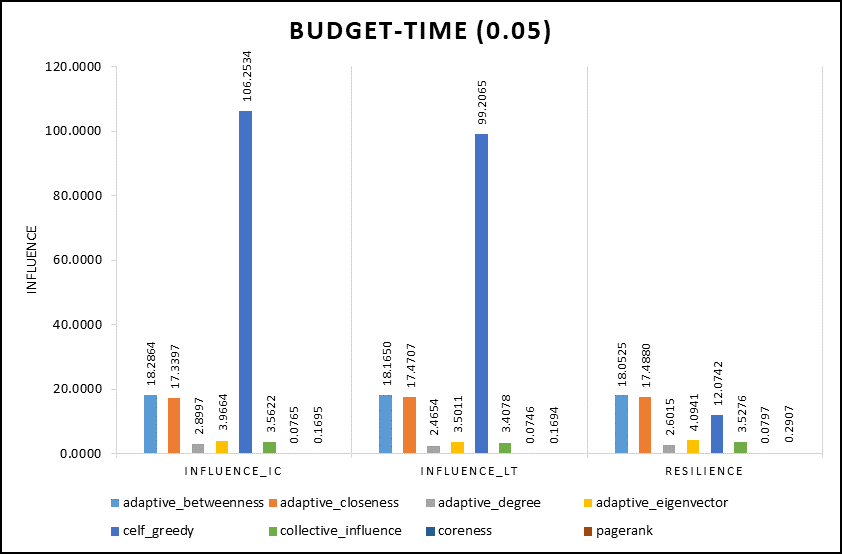
\includegraphics[angle=90, scale=0.65]{ita2000-budget-time-5}\par 
			\end{multicols}
			
			\caption{Normalized elapsed time for budget criteria on ITA-2000 network of influence mining papers.}
			\label{fig:inf-framework-ita2000-2}
		\end{figure*}
		
		\begin{figure*}[h]
			\begin{multicols}{2}
				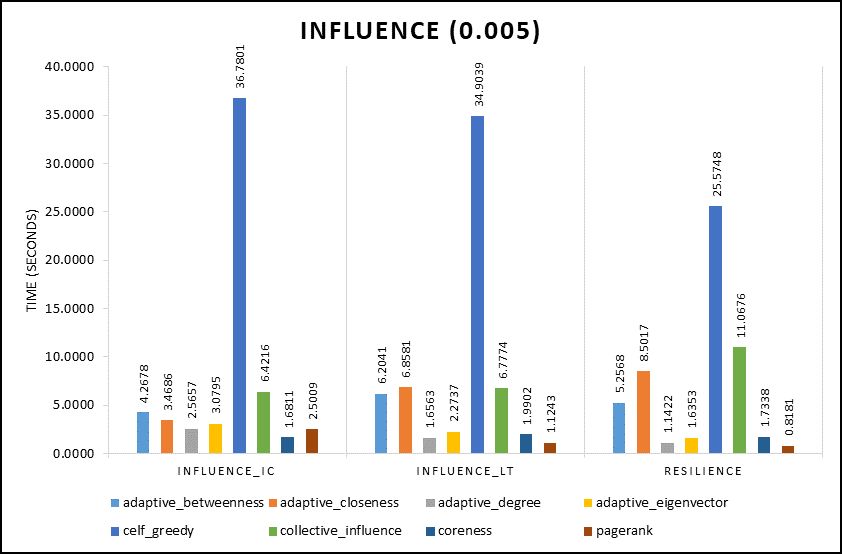
\includegraphics[angle=90, scale=0.65]{ita2000-influence-1}\par 
				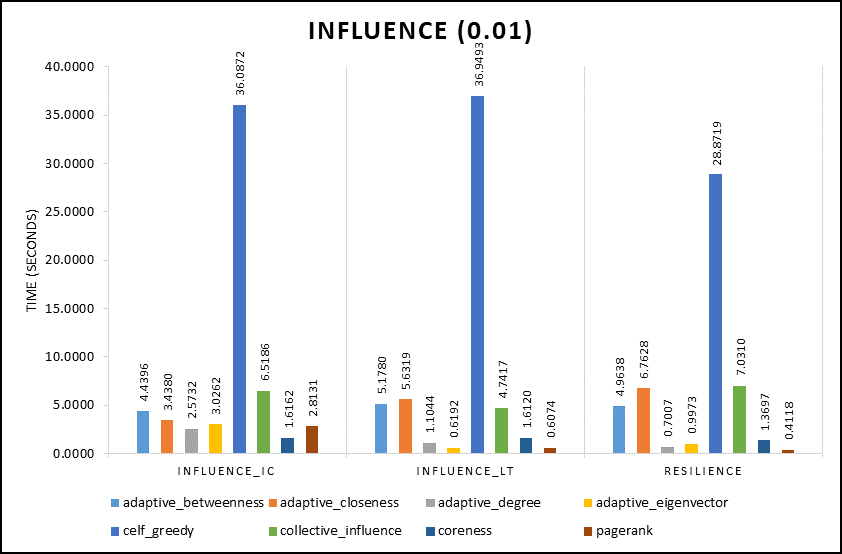
\includegraphics[angle=90, scale=0.65]{ita2000-influence-2}\par 
			\end{multicols}
			\begin{multicols}{2}
				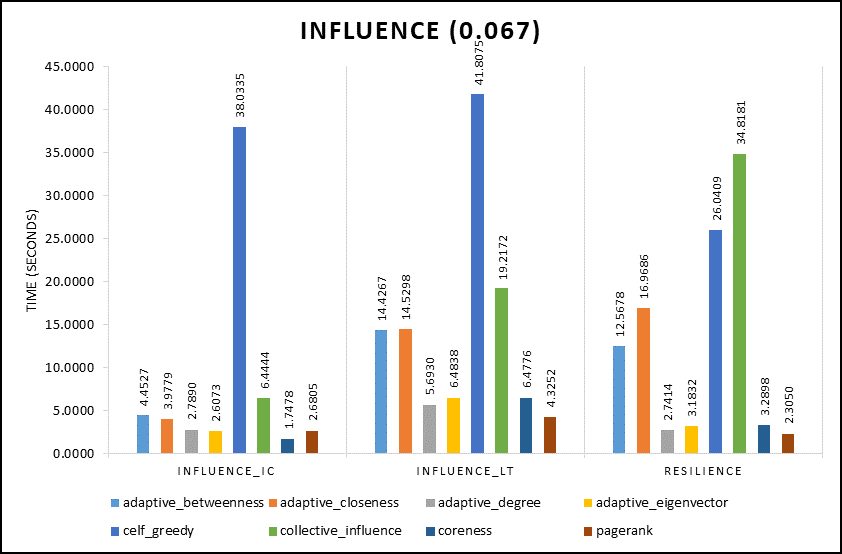
\includegraphics[angle=90, scale=0.65]{ita2000-influence-4}\par 
				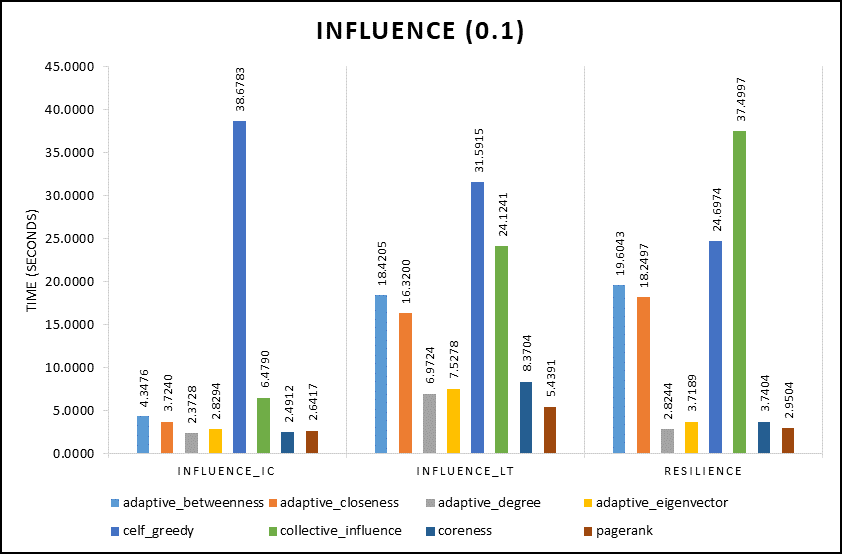
\includegraphics[angle=90, scale=0.65]{ita2000-influence-5}\par 
			\end{multicols}
			
			\caption{Normalized elapsed time for influence criteria on ITA-2000 network of influence mining papers.}
			\label{fig:inf-framework-ita2000-3}
		\end{figure*}
		
		
		% *** jdk6_dependencies ***
		\begin{figure*}[ht]
			\begin{multicols}{2}
				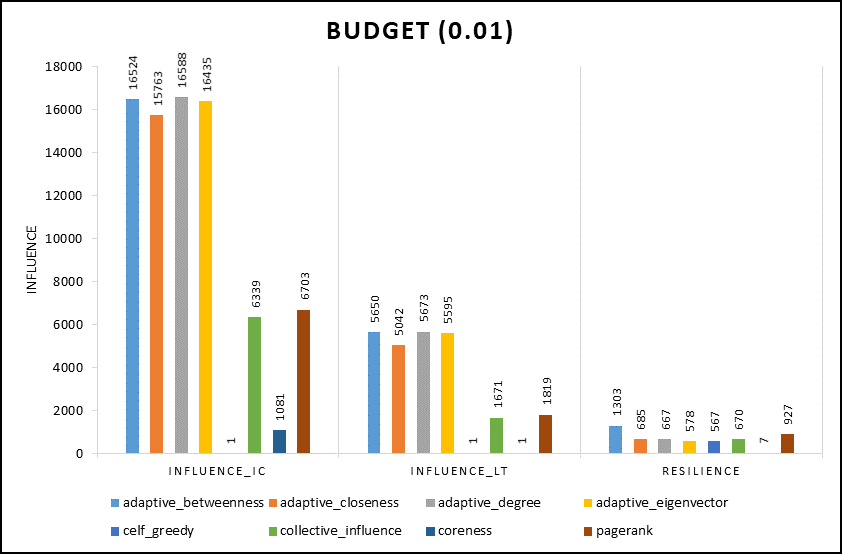
\includegraphics[angle=90, scale=0.65]{jdk6_dependencies-budget-1}\par 
				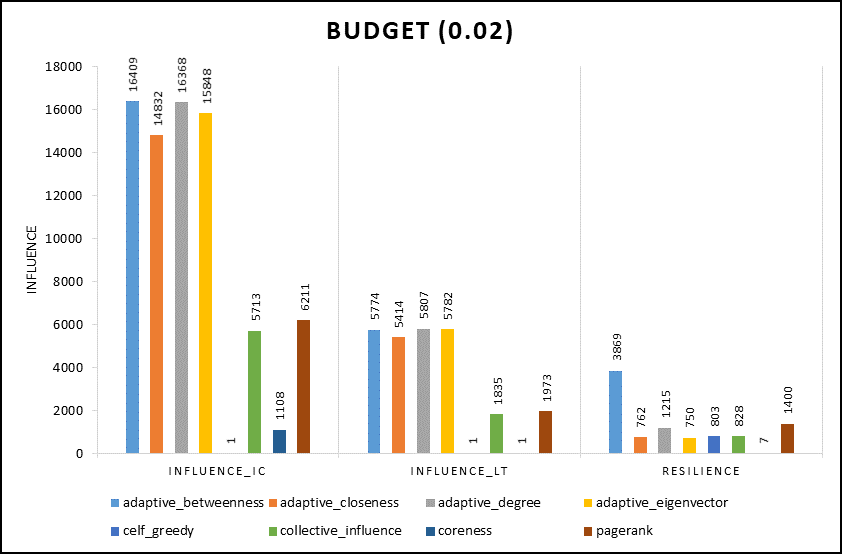
\includegraphics[angle=90, scale=0.65]{jdk6_dependencies-budget-2}\par 
			\end{multicols}
			\begin{multicols}{2}
				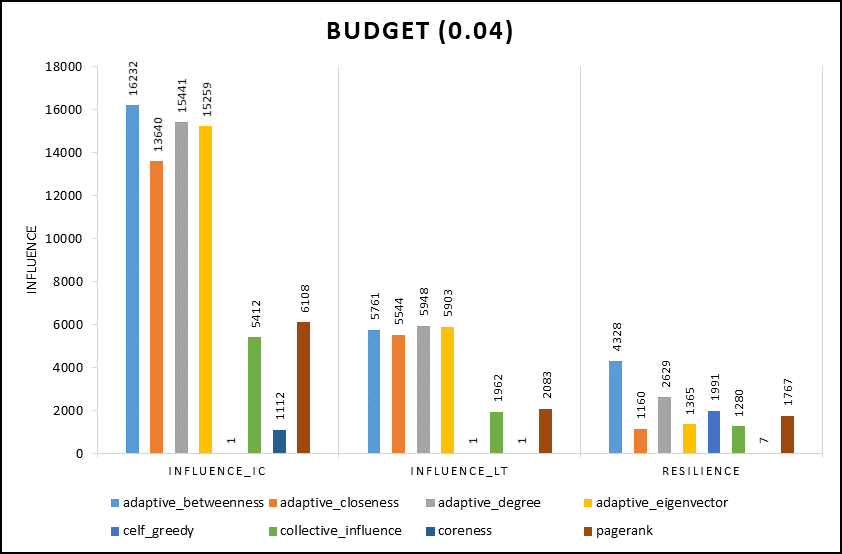
\includegraphics[angle=90, scale=0.65]{jdk6_dependencies-budget-4}\par 
				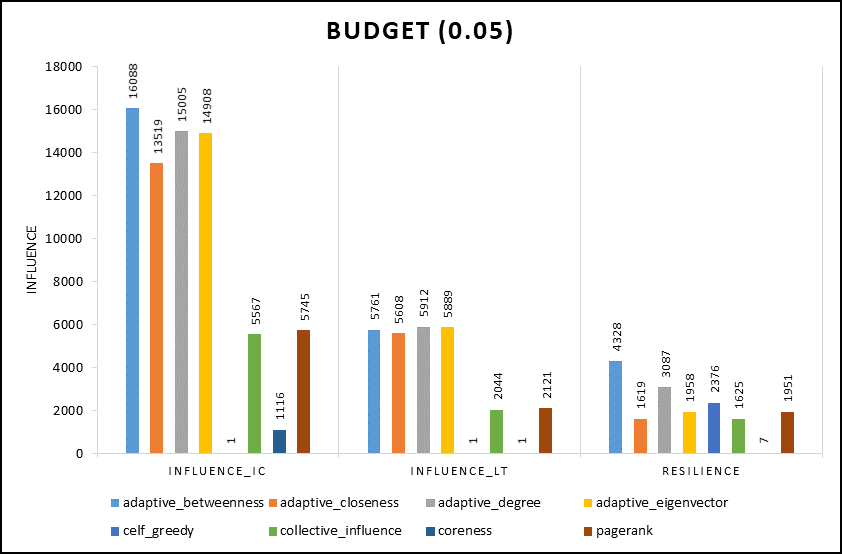
\includegraphics[angle=90, scale=0.65]{jdk6_dependencies-budget-5}\par 
			\end{multicols}
			
			\caption{Influence measure of JDK library dependency network of influence mining papers network on range on all budgets evaluated for all three tests.}
			\label{fig:inf-framework-jdk6_dependencies}
		\end{figure*}
		
		\begin{figure*}[ht]
			\begin{multicols}{2}
				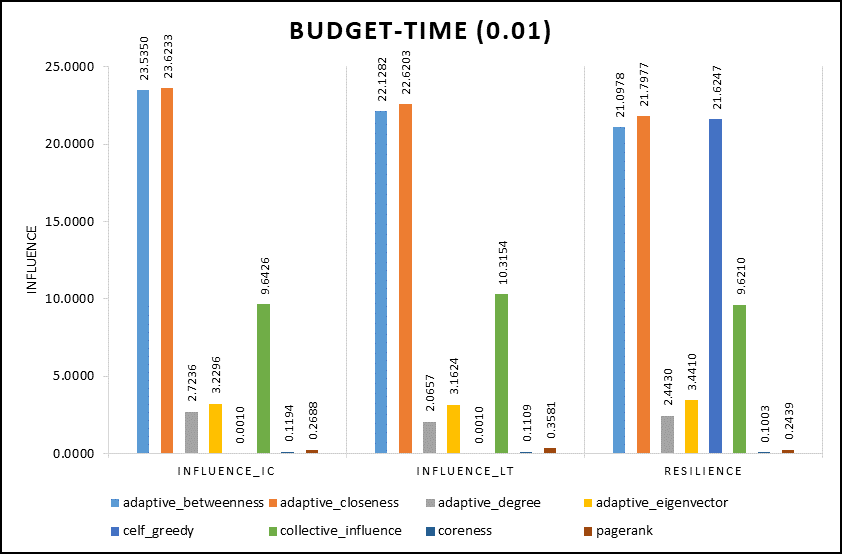
\includegraphics[angle=90, scale=0.65]{jdk6_dependencies-budget-time-1}\par 
				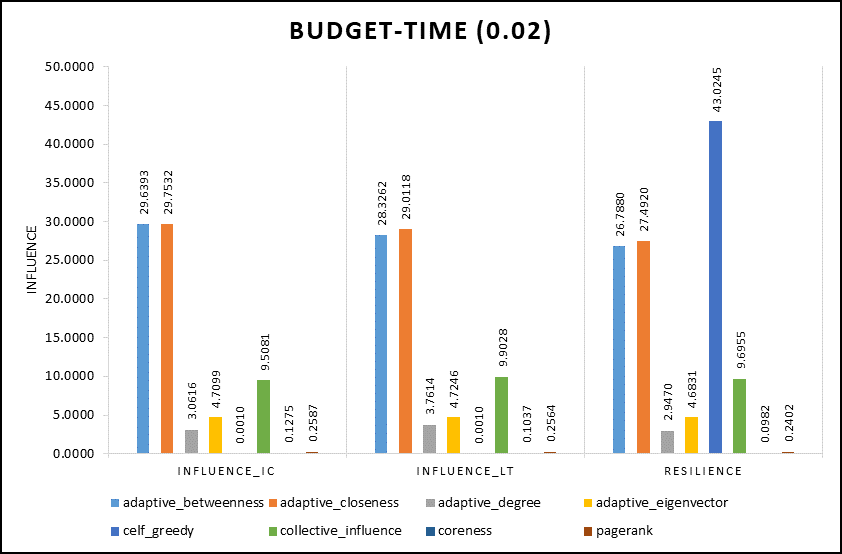
\includegraphics[angle=90, scale=0.65]{jdk6_dependencies-budget-time-2}\par 
			\end{multicols}
			\begin{multicols}{2}
				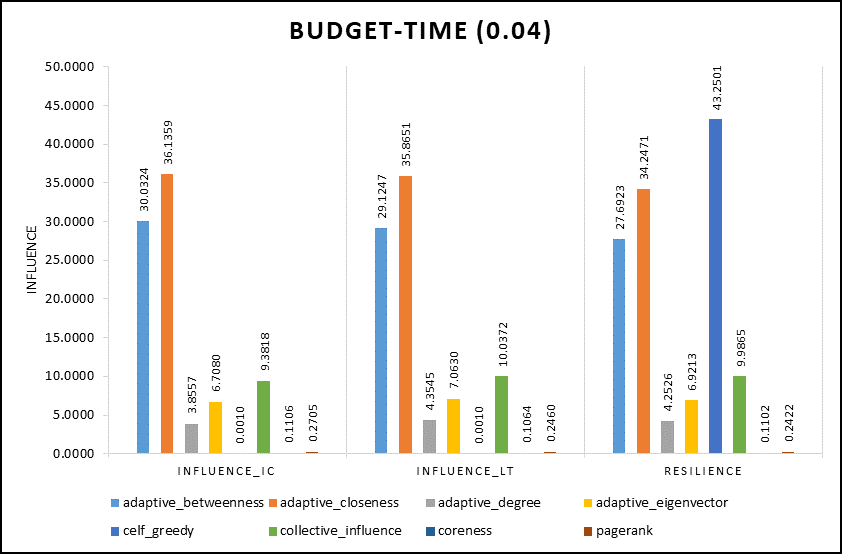
\includegraphics[angle=90, scale=0.65]{jdk6_dependencies-budget-time-4}\par 
				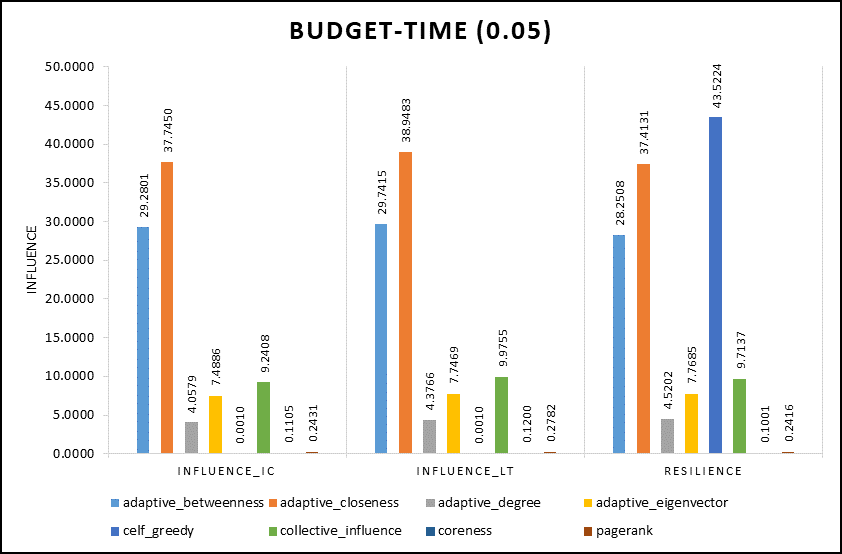
\includegraphics[angle=90, scale=0.65]{jdk6_dependencies-budget-time-5}\par 
			\end{multicols}
			
			\caption{Normalized elapsed time for budget criteria on JDK library dependency network of influence mining papers.}
			\label{fig:inf-framework-jdk6_dependencies2}
		\end{figure*}
		
		\begin{figure*}[h]
			\begin{multicols}{2}
				\includegraphics[angle=90, scale=0.65]{jdk6_dependencies-influence-1}\par 
				\includegraphics[angle=90, scale=0.65]{jdk6_dependencies-influence-2}\par 
			\end{multicols}
			\begin{multicols}{2}
				\includegraphics[angle=90, scale=0.65]{jdk6_dependencies-influence-4}\par 
				\includegraphics[angle=90, scale=0.65]{jdk6_dependencies-influence-5}\par 
			\end{multicols}
			
			\caption{Normalized elapsed time for influence criteria on JDK library dependency network of influence mining papers.}
			\label{fig:inf-framework-jdk6_dependencies3}
		\end{figure*}
		
		
		% *** karate ***
		\begin{figure*}[ht]
			\begin{multicols}{2}
				\includegraphics[angle=90, scale=0.65]{karate-budget-1}\par 
				\includegraphics[angle=90, scale=0.65]{karate-budget-2}\par 
			\end{multicols}
			\begin{multicols}{2}
				\includegraphics[angle=90, scale=0.65]{karate-budget-4}\par 
				\includegraphics[angle=90, scale=0.65]{karate-budget-5}\par 
			\end{multicols}
			
			\caption{Influence measure of Karate network of influence mining papers network on range on all budgets evaluated for all three tests.}
			\label{fig:inf-framework-karate}
		\end{figure*}
		
		\begin{figure*}[ht]
			\begin{multicols}{2}
				\includegraphics[angle=90, scale=0.65]{karate-budget-time-1}\par 
				\includegraphics[angle=90, scale=0.65]{karate-budget-time-2}\par 
			\end{multicols}
			\begin{multicols}{2}
				\includegraphics[angle=90, scale=0.65]{karate-budget-time-4}\par 
				\includegraphics[angle=90, scale=0.65]{karate-budget-time-5}\par 
			\end{multicols}
			
			\caption{Normalized elapsed time for budget criteria on Karate network of influence mining papers.}
			\label{fig:inf-framework-karate2}
		\end{figure*}
		
		\begin{figure*}[h]
			\begin{multicols}{2}
				\includegraphics[angle=90, scale=0.65]{karate-influence-1}\par 
				\includegraphics[angle=90, scale=0.65]{karate-influence-2}\par 
			\end{multicols}
			\begin{multicols}{2}
				\includegraphics[angle=90, scale=0.65]{karate-influence-4}\par 
				\includegraphics[angle=90, scale=0.65]{karate-influence-5}\par 
			\end{multicols}
			
			\caption{Normalized elapsed time for influence criteria on Karate network of influence mining papers.}
			\label{fig:inf-framework-karate3}
		\end{figure*}
		